\documentclass{book}

% Χρήση polyglossia για υποστήριξη ελληνικών (και αγγλικών, αν χρειαστεί)
\usepackage{polyglossia}
\setdefaultlanguage{greek}
\setotherlanguage{english}

% Ορισμός γραμματοσειρών για ελληνικά και αγγλικά
\newfontfamily\greekfont[Script=Greek]{Helvetica}
\newfontfamily\englishfont{Helvetica}
\newfontfamily\greekfonttt[Script=Greek]{Courier New}
\setmonofont{Courier New}[Scale=MatchLowercase]


\usepackage{listings}
\usepackage{xcolor}
\usepackage{geometry}
\usepackage{amsmath}
\usepackage{graphicx}
\usepackage{hyperref}
\usepackage{caption}
\usepackage{tcolorbox}
\usepackage{titlesec}
\usepackage{fancyhdr}
\usepackage{enumitem}
\usepackage{placeins}
\usepackage{helvet}    % Προαιρετική μοντέρνα sans-serif γραμματοσειρά
\usepackage{pagecolor}
\usepackage{framed}
\usepackage{csvsimple}       % For automatic CSV table creation
\usepackage{booktabs}        % For nicer table rules (\toprule, \midrule, etc.)

% Ρυθμίσεις σελίδας
\geometry{a4paper, margin=1in}

% Αφαίρεση πρόσθετου χρώματος από το περιβάλλον κώδικα
\lstset{
    backgroundcolor=\color{white},
    basicstyle=\ttfamily\small\color{black},
    frame=single,
    breaklines=true,
    showstringspaces=false,
    numbers=left,
    numberstyle=\tiny\color{black},
    keywordstyle=\color{black},
    commentstyle=\color{black},
    stringstyle=\color{black}
}

% Μορφοποίηση κεφαλαίων και ενοτήτων
\titleformat{\chapter}[display]
  {\normalfont\huge\bfseries}{\chaptertitlename\ \thechapter}{20pt}{\Huge}
\titlespacing*{\chapter}{0pt}{-20pt}{40pt}

\titleformat{\section}
  {\normalfont\Large\bfseries}{\thesection}{1em}{}

\pagestyle{fancy}
\fancyhead{}
\fancyfoot{}
\fancyhead[LE,RO]{\thepage}
\fancyhead[LO]{\textit{Αναλύσεις Ασκήσεων 1–6}}
\fancyhead[RE]{\textit{Θεωρία Μακροοικονομίας II}}
\renewcommand{\headrulewidth}{0.4pt}
\renewcommand{\footrulewidth}{0pt}

% Τίτλος, συγγραφέας, ημερομηνία
\title{\textbf{Ανάλυση Ασκήσεων 1--6} \\
\large Θεωρία Μακροοικονομίας II -- Άσκηση με Δεδομένα}
\author{Θεόδωρος Κούρταλης}
\date{\today}

\begin{document}

\maketitle
\tableofcontents
\newpage




\chapter{Επισκόπηση Κώδικα για τις Ασκήσεις 1--3}

\section{Φόρτωση Δεδομένων (Άσκηση 1)}
\begin{tcolorbox}[colback=white,colframe=black,title=Βασικός Κώδικας Python για Φόρτωση Αρχείου .mat]
\begin{lstlisting}[language=Python]
import scipy.io
import numpy as np

# ...
file_path = 'GDP_data.mat'
data = scipy.io.loadmat(file_path)

# Προβολή των μεταβλητών στο αρχείο .mat
mat_keys = [key for key in data.keys() if not key.startswith('__')]
print("Μεταβλητές στο .mat αρχείο:", mat_keys)

# Εξαγωγή κύριων σειρών
nominal_gdp = data['nominal_gdp']   # π.χ. (28, 2)
real_gdp    = data['real_gdp']      # π.χ. (28, 2)
gdp_index   = data['gdp_index']     # π.χ. (28, 2)
\end{lstlisting}
\end{tcolorbox}

\subsection*{Επεξήγηση}
\begin{itemize}
  \item Χρησιμοποιούμε την \texttt{scipy.io.loadmat} για διάβασμα δεδομένων από αρχείο \texttt{.mat}.
  \item Οι σειρές \textbf{Nominal GDP} και \textbf{Real GDP} θα αξιοποιηθούν στον υπολογισμό του αποπληθωριστή ΑΕΠ και στην επαλήθευση της σχέσης \(\Delta \log(\text{Nominal}) = \Delta \log(\text{Real}) + \Delta \log(\text{Deflator})\).
\end{itemize}

\section{Υπολογισμός Αποπληθωριστή και Φυσικών Λογαρίθμων (Άσκηση 1)}
\begin{tcolorbox}[colback=white,colframe=black,title=Υπολογισμός Αποπληθωριστή ΑΕΠ και Λογαρίθμων]
\begin{lstlisting}[language=Python]
# Υπολογισμός Αποπληθωριστή ως (Nominal / Real) * 100
gdp_deflator = (nominal_gdp / real_gdp) * 100

# Λήψη φυσικών λογαρίθμων
log_nominal_gdp = np.log(nominal_gdp)
log_real_gdp    = np.log(real_gdp)
log_deflator    = np.log(gdp_deflator)
\end{lstlisting}
\end{tcolorbox}

\subsection*{Επεξήγηση}
\begin{itemize}
  \item Ο \textbf{Αποπληθωριστής ΑΕΠ} προκύπτει από την αναλογία ονομαστικού προς πραγματικό ΑΕΠ επί 100.
  \item Έπειτα λαμβάνονται οι φυσικοί λογάριθμοι, ώστε ο υπολογισμός των ρυθμών μεταβολής (growth rates) να γίνει με διαφορές λογαρίθμων.
\end{itemize}

\section{Ρυθμοί Μεταβολής και Έλεγχος Ταυτότητας (Άσκηση 1)}
\begin{tcolorbox}[colback=white,colframe=black,title=Υπολογισμός Ρυθμών Μεταβολής και Επαλήθευση Ταυτότητας]
\begin{lstlisting}[language=Python]
# Ρυθμοί μεταβολής: πρώτες διαφορές των λογαρίθμων
growth_nominal_gdp = np.diff(log_nominal_gdp, axis=0)
growth_real_gdp    = np.diff(log_real_gdp, axis=0)
growth_deflator    = np.diff(log_deflator, axis=0)

# Έλεγχος ταυτότητας:
identity_diff = growth_nominal_gdp - (growth_real_gdp + growth_deflator)
max_identity_diff = np.max(np.abs(identity_diff))
print("Μεγ. απόκλιση από την ταυτότητα (πρέπει να είναι κοντά στο μηδέν):",
      max_identity_diff)
\end{lstlisting}
\end{tcolorbox}

\subsection*{Επεξήγηση}
\begin{itemize}
  \item \(\Delta \log(Y_t) = \log(Y_t) - \log(Y_{t-1})\). Η συνάρτηση \texttt{np.diff} υπολογίζει τη διαφορά ανάμεσα σε διαδοχικές γραμμές (στον άξονα 0).
  \item Η ταυτότητα \(\Delta \log(\text{Nominal GDP}) = \Delta \log(\text{Real GDP}) + \Delta \log(\text{GDP Deflator})\) ελέγχεται υπολογίζοντας την απόκλιση της αριστερής από τη δεξιά πλευρά.
\end{itemize}

\chapter{Εύρεση Έτους Βάσης (Άσκηση 2)}
\label{sec:exercise2}
\begin{tcolorbox}[colback=white,colframe=black,title=Βοηθητική Συνάρτηση για το Έτος Βάσης]
\begin{lstlisting}[language=Python]
def find_base_year(nominal, real):
    """
    Επιστρέφει το index στο οποίο το ονομαστικό ΑΕΠ
    προσεγγίζει καλύτερα το πραγματικό ΑΕΠ.
    """
    index = np.argmin(np.abs(nominal - real))
    return index

# Παράδειγμα χρήσης:
base_year_ea = find_base_year(nominal_gdp[:, 0], real_gdp[:, 0])
base_year_gr = find_base_year(nominal_gdp[:, 1], real_gdp[:, 1])
\end{lstlisting}
\end{tcolorbox}

\subsection*{Επεξήγηση}
\begin{itemize}
  \item Το \textbf{έτος βάσης} αντιστοιχεί συνήθως στο σημείο όπου το ονομαστικό ΑΕΠ ισούται (ή βρίσκεται πιο κοντά) στο πραγματικό ΑΕΠ.
  \item Η συνάρτηση \texttt{argmin} βρίσκει τη θέση ελάχιστης απόκλισης \(|Y_t - y_t|\).
\end{itemize}

\chapter{Δημιουργία Διαγραμμάτων σε Subplots (Άσκηση 3)}

\section{Συνάρτηση για Σχεδιασμό των Ρυθμών Μεταβολής}
\begin{tcolorbox}[colback=white,colframe=black,title=Παραγωγή Τριών Subplots για Κάθε Περιοχή/Χώρα]
\begin{lstlisting}[language=Python]
def plot_growth_subplots(nom_growth, real_growth, defl_growth, country, filename_prefix='plot'):
    """
    Δημιουργεί σχήμα με 3 subplots:
       1) Ρυθμός μεταβολής Ονομαστικού ΑΕΠ
       2) Ρυθμός μεταβολής Πραγματικού ΑΕΠ
       3) Ρυθμός μεταβολής Αποπληθωριστή ΑΕΠ
    """
    import matplotlib.pyplot as plt
    
    # Παράδειγμα χρονικού εύρους (αν τα δεδομένα ξεκινούν π.χ. το 1996)
    years = range(1996, 1996 + len(nom_growth))
    
    fig, axs = plt.subplots(3, 1, figsize=(8, 10), dpi=150)

    axs[0].plot(years, nom_growth, marker='o')
    axs[0].set_title(f'{country} - Ρυθμός Μεταβολής Ονομ. ΑΕΠ (Δ log(Yₜ))')
    
    axs[1].plot(years, real_growth, marker='s')
    axs[1].set_title(f'{country} - Ρυθμός Μεταβολής Πραγμ. ΑΕΠ (Δ log(yₜ))')
    
    axs[2].plot(years, defl_growth, marker='^')
    axs[2].set_title(f'{country} - Ρυθμός Μεταβολής Αποπληθωριστή (Δ log(Pₜ))')

    fig.tight_layout()
    plt.savefig(f'{filename_prefix}.png')
    plt.close()
\end{lstlisting}
\end{tcolorbox}

\subsection*{Επεξήγηση}
\begin{itemize}
  \item Με την παραπάνω συνάρτηση δημιουργούνται τρία διαδοχικά διαγράμματα (subplots), το καθένα για έναν διαφορετικό ρυθμό μεταβολής (nominal, real, deflator).
  \item Το εύρος των ετών προσαρμόζεται κατάλληλα, ανάλογα με το πόσα σημεία υπάρχουν στη μεταβλητή των ρυθμών μεταβολής.
\end{itemize}
\begin{tcolorbox}[colback=white,colframe=black,title= Διάγραμμα Ρυθμών Μεταβολής]
  \centering
  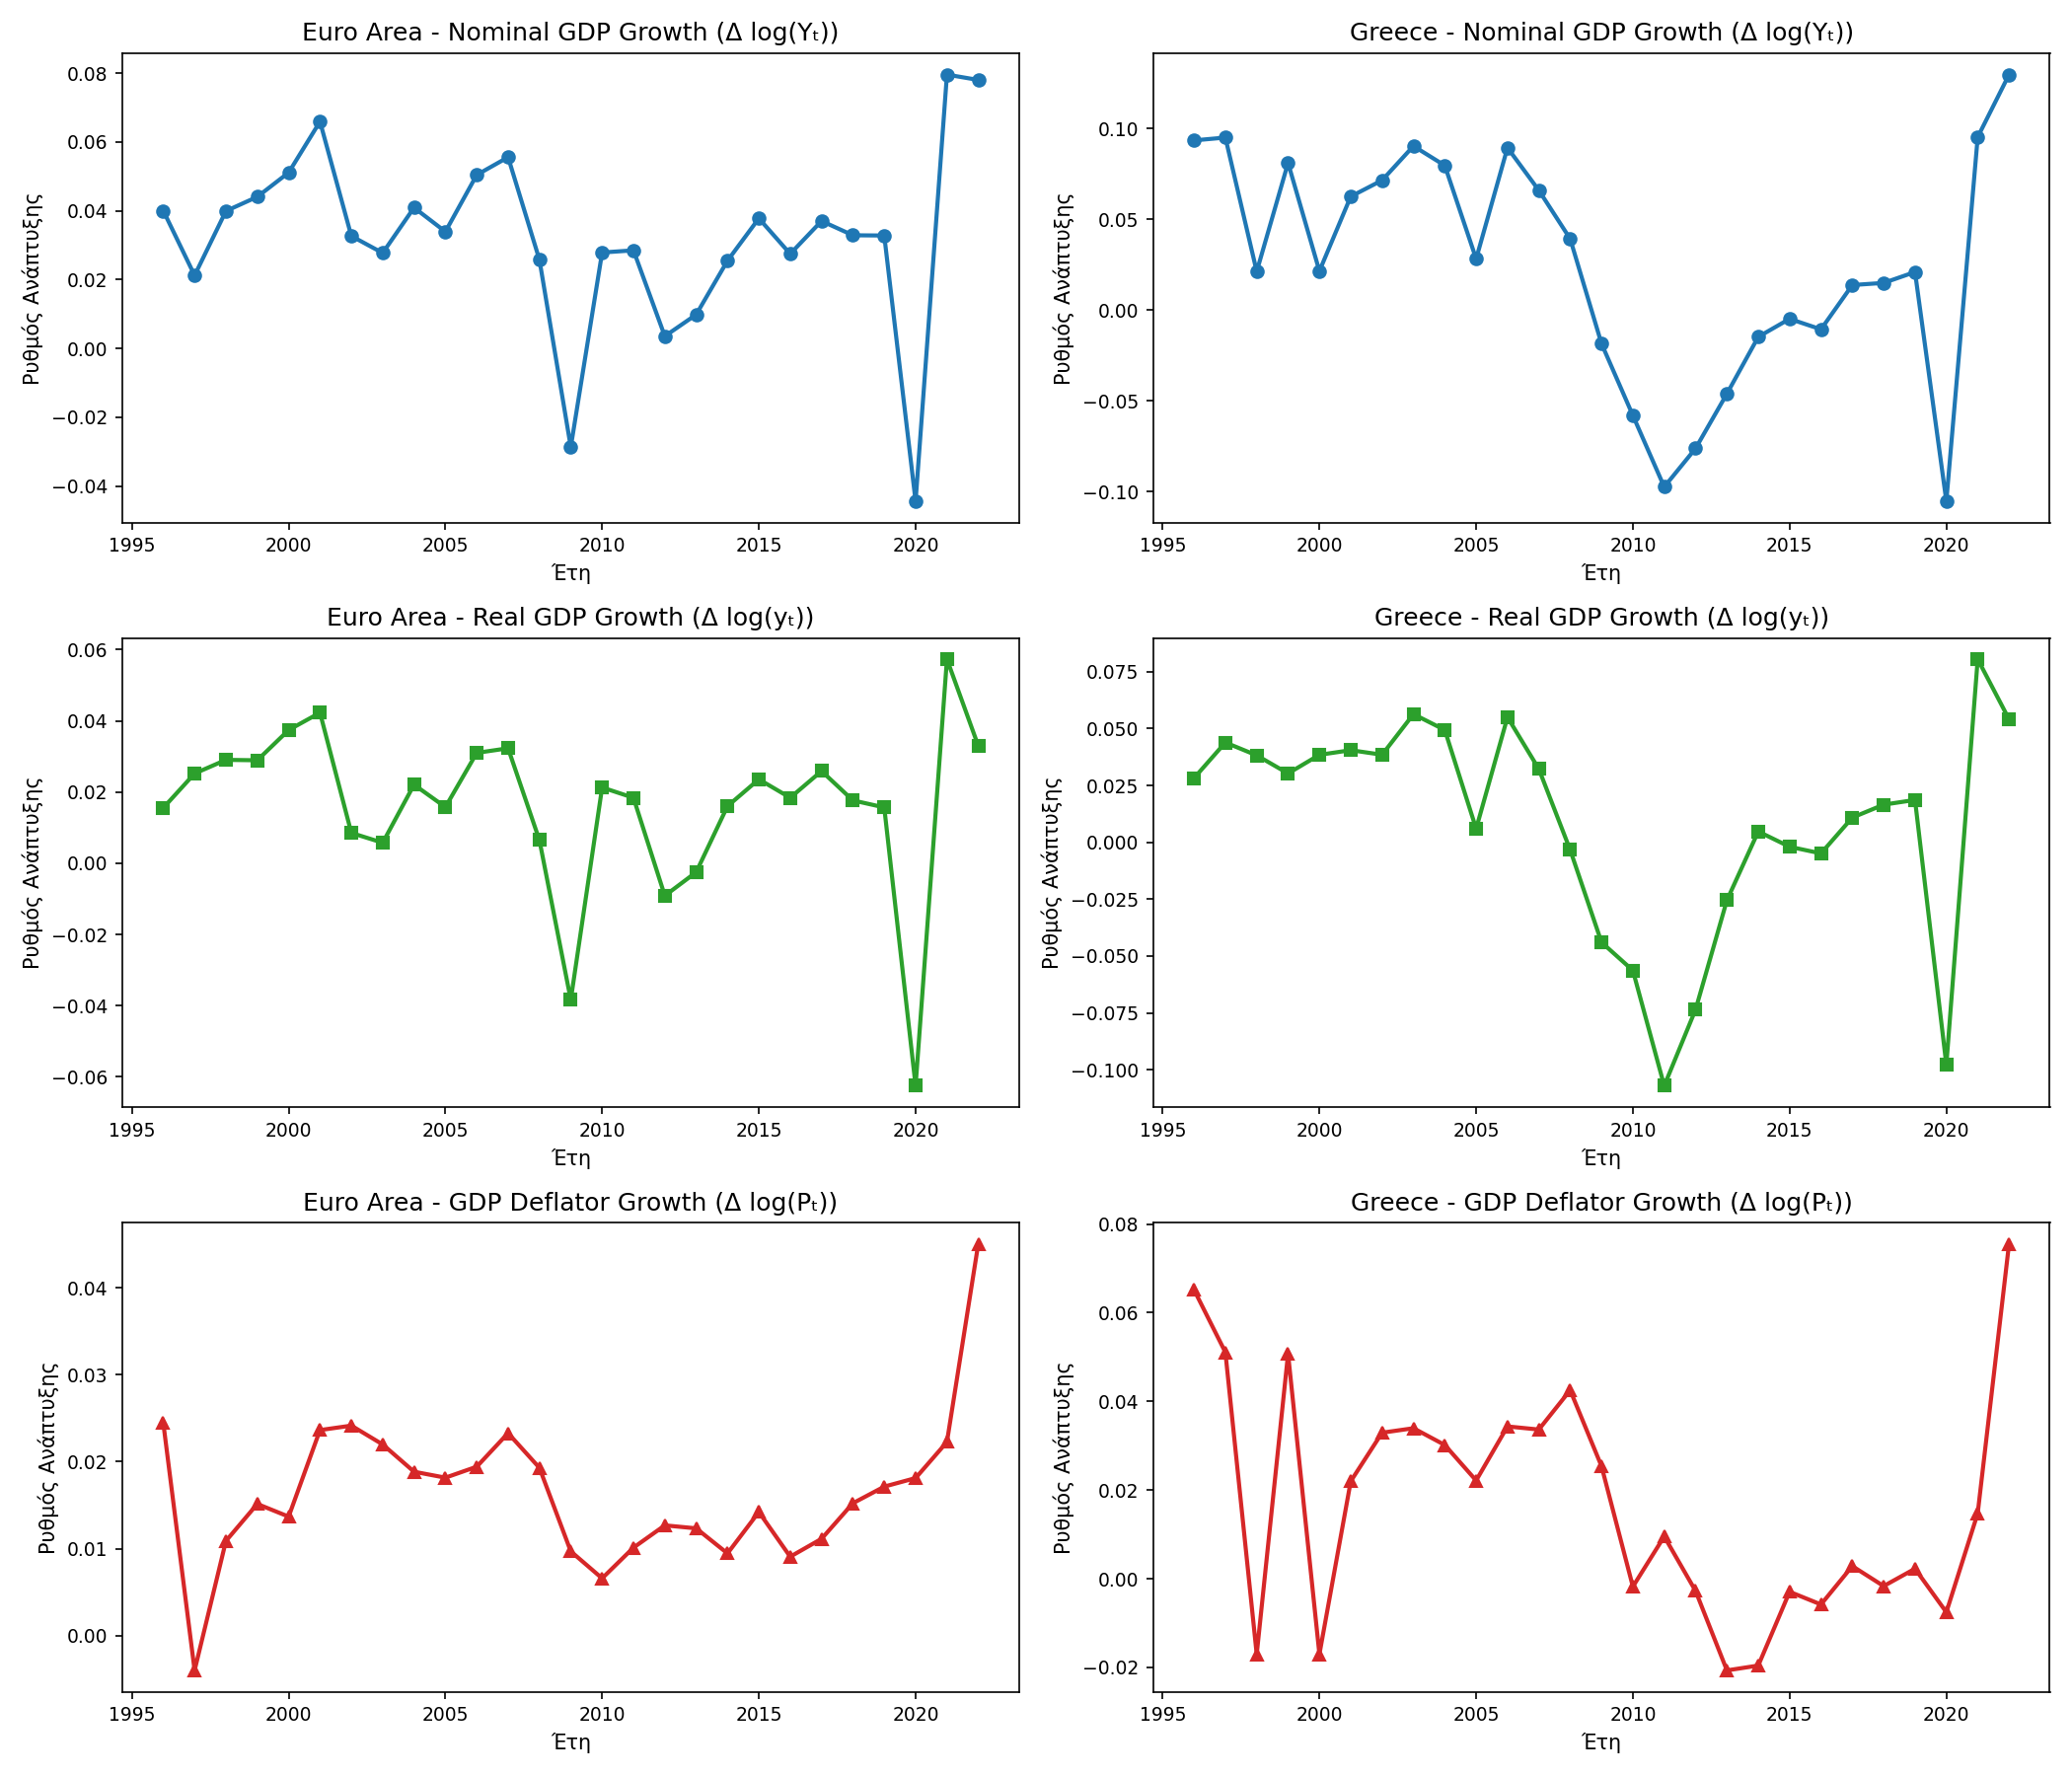
\includegraphics[width=0.8\textwidth]{/Users/thodoreskourtales/TK.MT.1/exercise.1-3/side_by_side_growth.png}
  \vspace{0.5em}
  \captionof{figure}{Διάγραμμα με τους ρυθμούς μεταβολής για τις δύο χώρες.}
\end{tcolorbox}
\chapter{Εισαγωγή στην Άσκηση 4 (Ετήσια Δεδομένα)}
Στην παρούσα άσκηση επεξεργαζόμαστε \textbf{ετήσια} μακροοικονομικά δεδομένα για την Ευρωζώνη και την Ελλάδα, εφαρμόζοντας τεχνικές που είδαμε στις προηγούμενες ασκήσεις:
\begin{itemize}
    \item Χρήση ονομαστικών (\emph{Nominal}) και αλυσοδεμένων (\emph{Chain linked}) τιμών από αρχείο Excel.
    \item Υπολογισμός αποπληθωριστή \(\bigl(\text{Deflator} = \frac{\text{Nominal}}{\text{Chain linked}}\times 100\bigr)\).
    \item Λήψη λογαρίθμων και υπολογισμός ρυθμών μεταβολής \(\bigl(\Delta \log\bigr)\).
    \item Παρουσίαση διαγραμμάτων ρυθμών μεταβολής καθώς και συνδυασμένων διαγραμμάτων (Nominal, Chain, Deflator) κανονικοποιημένων σε ένα \emph{έτος βάσης} (π.χ. 2015).
\end{itemize}

Ακολουθεί ο κώδικας Python που υλοποιεί τα παραπάνω βήματα σε επιμέρους τμήματα, με σύντομες επεξηγήσεις.


\section{Φόρτωση Βιβλιοθηκών και Λεξικό \texttt{sheet\_info}}
Σε αυτό το πρώτο κομμάτι κώδικα:
\begin{enumerate}
    \item Εισάγουμε τις βασικές βιβλιοθήκες \texttt{pandas}, \texttt{numpy} και \texttt{matplotlib}.
    \item Ορίζουμε ένα λεξικό \texttt{sheet\_info} που καθορίζει για κάθε μεταβλητή (π.χ. \emph{Nominal GDP}, \emph{Exports} κ.λπ.) τα φύλλα Excel (\emph{Nominal}, \emph{Chain linked}) από όπου θα αντλήσουμε τα δεδομένα.
\end{enumerate}

\begin{tcolorbox}[colback=white,colframe=black,title=Φόρτωση Βιβλιοθηκών \& Εισαγωγή \texttt{sheet\_info}]
\begin{lstlisting}[language=Python]
#!/usr/bin/env python3
# -*- coding: utf-8 -*-
"""
Created on Thu Mar 13 16:47:30 2025
@author: thodoreskourtales
"""

import pandas as pd
import numpy as np
import matplotlib.pyplot as plt
import os

# Για κάθε μεταβλητή, ορίζουμε ποιο φύλλο του Excel περιέχει Nominal τιμές
# και ποιο φύλλο περιέχει αλυσοδεμένες (Chain linked) πραγματικές τιμές.
sheet_info = {
    "Nominal GDP": {
        "Nominal": "Sheet 40",          # Current prices, million euro (Gross domestic product at market prices)
        "Chain linked": "Sheet 79"       # Chain linked volumes, index 2015=100 (Gross domestic product at market prices)
    },
    "Final consumption expenditure": {
        "Nominal": "Sheet 42",           # Current prices, million euro (Final consumption expenditure)
        "Chain linked": "Sheet 81"       # Chain linked volumes, index 2015=100 (Final consumption expenditure)
    },
    "Final consumption expenditure of general government": {
        "Nominal": "Sheet 43",           # Current prices, million euro (Final consumption expenditure of general government)
        "Chain linked": "Sheet 82"       # Chain linked volumes, index 2015=100 (Final consumption expenditure of general government)
    },
    "Final consumption expenditure of households": {
        "Nominal": "Sheet 47",           # Current prices, million euro (Final consumption expenditure of households)
        "Chain linked": "Sheet 86"       # Chain linked volumes, index 2015=100 (Final consumption expenditure of households)
    },
    "Gross fixed capital formation": {
        "Nominal": "Sheet 51",           # Current prices, million euro (Gross fixed capital formation)
        "Chain linked": "Sheet 90"       # Chain linked volumes, index 2015=100 (Gross fixed capital formation)
    },
    "Exports of goods and services": {
        "Nominal": "Sheet 55",           # Current prices, million euro (Exports of goods and services)
        "Chain linked": "Sheet 94"       # Chain linked volumes, index 2015=100 (Exports of goods and services)
    },
    "Imports of goods and services": {
        "Nominal": "Sheet 58",           # Current prices, million euro (Imports of goods and services)
        "Chain linked": "Sheet 97"       # Chain linked volumes, index 2015=100 (Imports of goods and services)
    }
}

\end{lstlisting}
\end{tcolorbox}

\subsection*{Επεξήγηση}
\begin{itemize}
    \item Η μεταβλητή \texttt{sheet\_info} διευκολύνει την \emph{αυτοματοποιημένη} επεξεργασία πολλαπλών οικονομικών μεγεθών, καθώς τα δεδομένα διαβάζονται από διαφορετικά φύλλα του ίδιου Excel.
    \item Η βιβλιοθήκη \texttt{os} χρησιμοποιείται σε περίπτωση που θέλουμε να αποθηκεύουμε τα διαγράμματα σε κάποιον συγκεκριμένο υποφάκελο.

\end{itemize}

\section{Βοηθητικές Συναρτήσεις}
Ακολουθούν συναρτήσεις που εκτελούν διακριτά βήματα: μετατροπή δεδομένων σε \texttt{float}, υπολογισμό/απεικόνιση ρυθμών μεταβολής (\(\Delta \log\)), δημιουργία διαγραμμάτων \emph{combined} (Nominal, Chain linked, Deflator) κ.λπ.

\subsection{Μετατροπή σε \texttt{float} \& Συναρτήσεις Πλοκής}
\begin{tcolorbox}[colback=white,colframe=black,title=convert\_to\_float \& Συναρτήσεις Διαγραμμάτων (Side by Side / Combined)]
\begin{lstlisting}[language=Python]
def convert_to_float(x):
    """
    Μετατρέπει την τιμή κελιού σε float.
    Αν συναντήσει τον συμβολισμό ':' (Eurostat για ελλιπή δεδομένα),
    επιστρέφει NaN.
    """
    try:
        if isinstance(x, str):
            x = x.strip()
            if x == ":":
                return np.nan
        return float(x)
    except:
        return np.nan


def plot_growth_side_by_side(years, growth_values, var_name, filename, scale_threshold=2):
    """
    Δημιουργεί δύο υποδιαγράμματα (Euro Zone, Greece) για τους ρυθμούς μεταβολής,
    όπου growth_values[:,0] αναφέρεται στην Ευρωζώνη και growth_values[:,1] στην Ελλάδα.
    """
    std_first = np.nanstd(growth_values[:, 0])
    std_second = np.nanstd(growth_values[:, 1])
    # Αν η διακύμανση της Ελλάδας είναι πολύ μεγαλύτερη, μη μοιράζεσαι το ίδιο y-axis.
    if std_second > scale_threshold * std_first:
        fig, axs = plt.subplots(1, 2, figsize=(12, 5), dpi=150)
    else:
        fig, axs = plt.subplots(1, 2, figsize=(12, 5), dpi=150, sharey=True)
    
    ...
    # Απόσπασμα κώδικα παραλείπεται για συντομία
    ...
\end{lstlisting}
\end{tcolorbox}

\subsection*{Επεξήγηση}
\begin{itemize}
    \item \textbf{\texttt{convert\_to\_float}}: Μετατρέπει σε αριθμητική τιμή και αντικαθιστά τυχόν μη αριθμητικά στοιχεία (π.χ. «:») με \texttt{NaN}.
    \item \textbf{\texttt{plot\_growth\_side\_by\_side}}: Παρουσιάζει τους ετήσιους ρυθμούς μεταβολής μιας μεταβλητής σε δύο διαγράμματα (Euro Zone, Greece). Εάν τα δεδομένα της Ελλάδας εμφανίζουν πολύ μεγαλύτερη διακύμανση, το \texttt{sharey} απενεργοποιείται, ώστε το διάγραμμα της Ευρωζώνης να μην «συμπιέζεται».
    \item \textbf{\texttt{plot\_measure\_combined}}: Σχεδιάζει τις σειρές \emph{Nominal, Real, Deflator} κανονικοποιημένες σε 100 σε κάποιο έτος βάσης, ώστε να συγκρίνονται ευκολότερα.

\end{itemize}

\subsection{Συνάρτηση για Συνδυαστική Πλοκή Ρυθμού Μεταβολής (Nominal, Chain, Deflator) ανά Χώρα}

\begin{tcolorbox}[colback=white,colframe=black,title=plot\_measure\_growth\_by\_country]
\begin{lstlisting}[language=Python]
def plot_measure_growth_by_country(measure_name, years,
                                   growth_nominal, growth_chain, growth_deflator,
                                   filename_euro, filename_greece):
    """
    Δημιουργεί δύο ξεχωριστά διαγράμματα (ένα για Euro Zone και ένα για Greece),
    παρουσιάζοντας Nominal Growth, Chain Growth και Deflator Growth μαζί.
    """

    # --- Euro Zone ---
    plt.figure(figsize=(10, 6), dpi=150)
    plt.plot(years, growth_nominal[:, 0], marker='o', linestyle='-',
             label=f"{measure_name} Nominal Growth")
    plt.plot(years, growth_chain[:, 0], marker='s', linestyle='-',
             label=f"{measure_name} Chain Growth")
    plt.plot(years, growth_deflator[:, 0], marker='^', linestyle='-',
             label=f"{measure_name} Deflator Growth")
    plt.title(f"Combined Growth Rates ({measure_name}) – Euro Zone")
    plt.xlabel("Year")
    plt.ylabel("Growth Rate (Δ log(series))")
    plt.legend()
    plt.tight_layout()
    plt.savefig(filename_euro)
    plt.close()
    print(f"Combined growth plot for '{measure_name}' (Euro Zone) saved as: {filename_euro}")

    # --- Greece ---
    plt.figure(figsize=(10, 6), dpi=150)
    plt.plot(years, growth_nominal[:, 1], marker='o', linestyle='-',
             label=f"{measure_name} Nominal Growth")
    plt.plot(years, growth_chain[:, 1], marker='s', linestyle='-',
             label=f"{measure_name} Chain Growth")
    plt.plot(years, growth_deflator[:, 1], marker='^', linestyle='-',
             label=f"{measure_name} Deflator Growth")
    plt.title(f"Combined Growth Rates ({measure_name}) – Greece")
    plt.xlabel("Year")
    plt.ylabel("Growth Rate (Δ log(series))")
    plt.legend()
    plt.tight_layout()
    plt.savefig(filename_greece)
    plt.close()
    print(f"Combined growth plot for '{measure_name}' (Greece) saved as: {filename_greece}")
\end{lstlisting}
\end{tcolorbox}

\subsection*{Επεξήγηση}
Η \texttt{plot\_growth\_side\_by\_side} δημιουργεί δύο υποδιαγράμματα για \emph{μία} μόνο μεταβλητή (π.χ. Nominal), ενώ η \texttt{plot\_measure\_growth\_by\_country} φτιάχνει \emph{δύο} ξεχωριστά διαγράμματα (Euro Zone, Greece) για \emph{όλες} τις μεταβλητές μαζί (Nominal, Chain, Deflator).

\section{Κύριο Τμήμα Κώδικα (\texttt{main})}
Στο κύριο μέρος (\texttt{main}):
\begin{enumerate}
    \item Διαβάζουμε τα φύλλα Excel (\emph{Nominal}, \emph{Chain linked}) που ορίζει το \texttt{sheet\_info}.
    \item Εντοπίζουμε τις στήλες που αντιστοιχούν στα έτη 1995–2022.
    \item Εφαρμόζουμε τις βοηθητικές συναρτήσεις για να δημιουργηθούν τα επιμέρους διαγράμματα ρυθμών μεταβολής και επίπεδων.
    \item Καταγράφουμε σε ένα λεξικό \texttt{report\_data} στοιχεία που μπορεί να χρειαστούμε για περαιτέρω επεξεργασία (π.χ. μέσοι ρυθμοί, ονόματα αρχείων PNG).
\end{enumerate}

\begin{tcolorbox}[colback=white,colframe=black,title=Κύρια Συνάρτηση \texttt{main} (Άσκηση 4)]
\begin{lstlisting}[language=Python]
# Λεξικό για να αποθηκεύουμε πληροφορίες (π.χ. μέσους ρυθμούς).
report_data = {}

def main():
    # Διατρέχει κάθε μεταβλητή (measure_name) στο sheet_info.
    for measure_name, sheets in sheet_info.items():
        try:
            # Διαβάζει ονομαστικές τιμές
            df_nom = pd.read_excel("Annual_Data.xlsx",
                                   sheet_name=sheets["Nominal"],
                                   header=None, skiprows=8, nrows=4)
            # Διαβάζει αλυσοδεμένες τιμές
            df_chain = pd.read_excel("Annual_Data.xlsx",
                                     sheet_name=sheets["Chain linked"],
                                     header=None, skiprows=8, nrows=4)
        except Exception as e:
            print(f"Error reading sheets for {measure_name}: {e}")
            continue
        
        ...
        # Υπολογισμοί, δημιουργία μεταβλητών, διαγραμμάτων κ.λπ.
        ...
        
        # Πλοκή ρυθμών (ονομαστικού, αλυσοδεμένου, αποπληθωριστή)
        filename_nom_growth = (measure_name.replace(" ", "_")
                               .replace("/", "_") 
                               + "_nominal_growth.png")
        plot_growth_side_by_side(growth_years, growth_nom, 
                                 measure_name + " Nominal", 
                                 filename_nom_growth)

        filename_chain_growth = (measure_name.replace(" ", "_")
                                 .replace("/", "_") 
                                 + "_chain_growth.png")
        ...
        # Παρόμοια για deflator και combined plots
        ...
    
    # Εκτύπωση περίληψης για όλες τις μεταβλητές που επεξεργαστήκαμε
    print("\nProcessing completed. Summary of measures:")
    for measure, info in report_data.items():
        print(f"\n{measure}:")
        for key, value in info.items():
            print(f"  {key}: {value}")

if __name__ == "__main__":
    main()
\end{lstlisting}
\end{tcolorbox}

\subsection*{Επεξήγηση}
\begin{itemize}
    \item Γίνεται συστηματική ανάγνωση των \textbf{Nominal} και \textbf{Chain linked} φύλλων για κάθε μεταβλητή.
    \item Εξάγονται τα δεδομένα για δύο σειρές (Euro Zone, Greece), φιλτράροντας τις στήλες με τα έτη [1995, 2022].
    \item Υπολογίζεται \textbf{Αποπληθωριστής} ως \(\frac{\text{Nominal}}{\text{Chain linked}} \times 100\), λαμβάνονται λογάριθμοι και κατόπιν υπολογίζονται \emph{ρυθμοί μεταβολής} (\(\Delta \log(\cdot)\)).
    \item Οι συναρτήσεις \texttt{plot\_growth\_side\_by\_side}, \texttt{plot\_measure\_combined} και \texttt{plot\_measure\_growth\_by\_country} δημιουργούν και αποθηκεύουν τα διαγράμματα (PNG) για περαιτέρω χρήση.
    \item Το \texttt{report\_data} μπορεί να περιέχει, μεταξύ άλλων, μέσους ρυθμούς ανάπτυξης ή άλλα στατιστικά για εύκολη αναφορά.

\end{itemize}

\section{Παράρτημα: Παραγόμενα Διαγράμματα}

\graphicspath{{/Users/thodoreskourtales/TK.MT.1/exercise.4/}}

% ---------------------------------------------
% ΔΙΟΡΘΩΜΕΝΟΙ ΤΙΤΛΟΙ ΣΤΑ ΠΛΑΙΣΙΑ (Tcolorbox)
% ---------------------------------------------

\begin{tcolorbox}[colback=white,colframe=black,title={Εξαγωγές αγαθών και υπηρεσιών: ανάπτυξη αλυσίδας}]
  \centering
  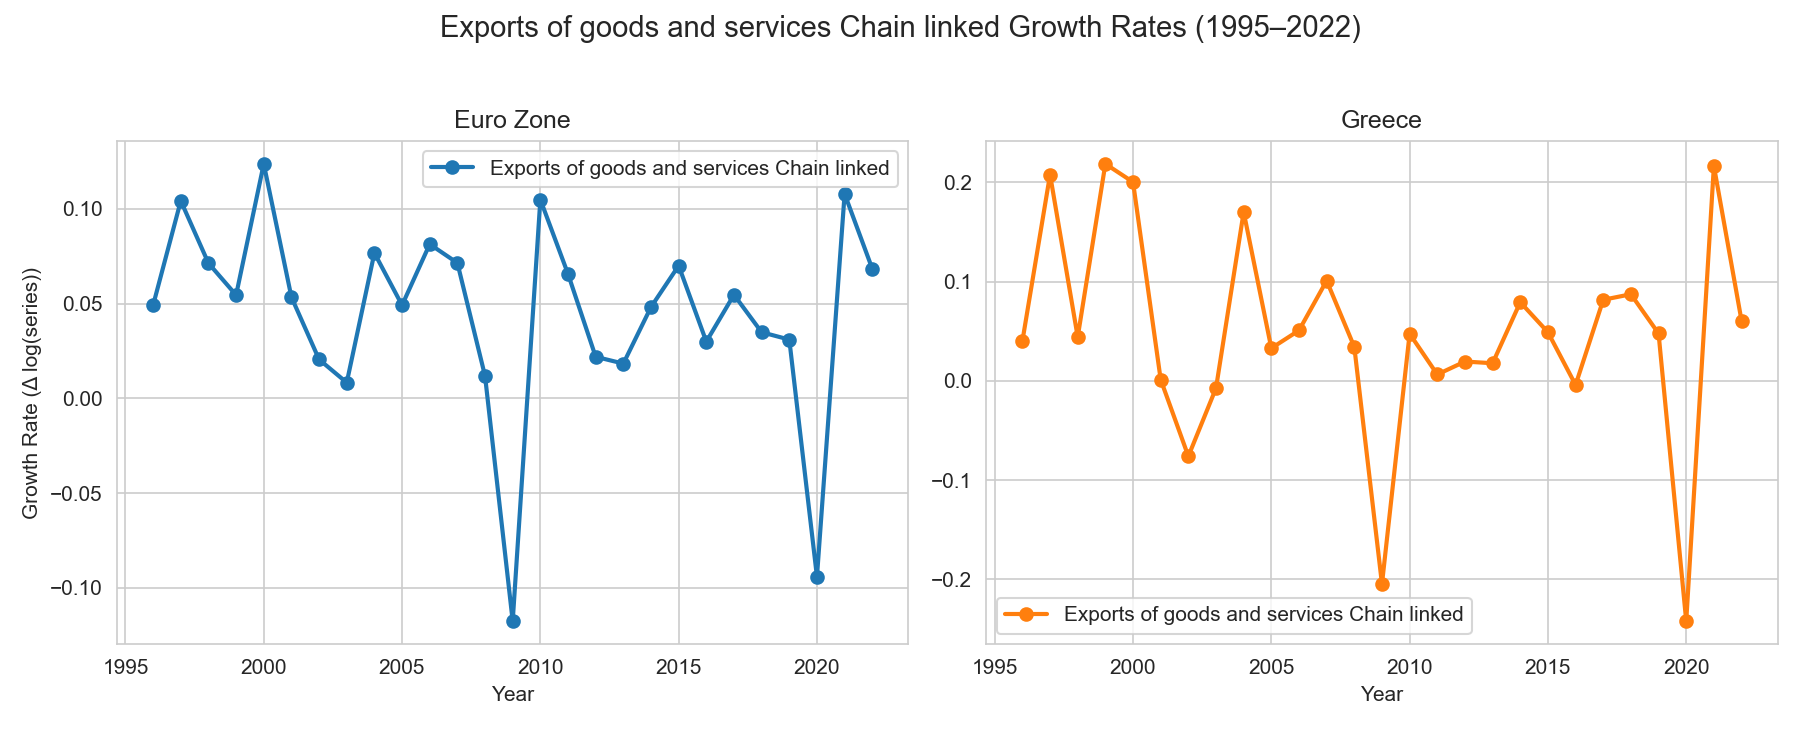
\includegraphics[width=0.8\textwidth]{Exports_of_goods_and_services_chain_growth.png}
  \vspace{0.5em}

\captionof{figure}{}\end{tcolorbox}
\FloatBarrier

\begin{tcolorbox}[colback=white,colframe=black,title={Εξαγωγές αγαθών και υπηρεσιών: συνδυασμένη ανάπτυξη στην Ευρωζώνη}]
  \centering
  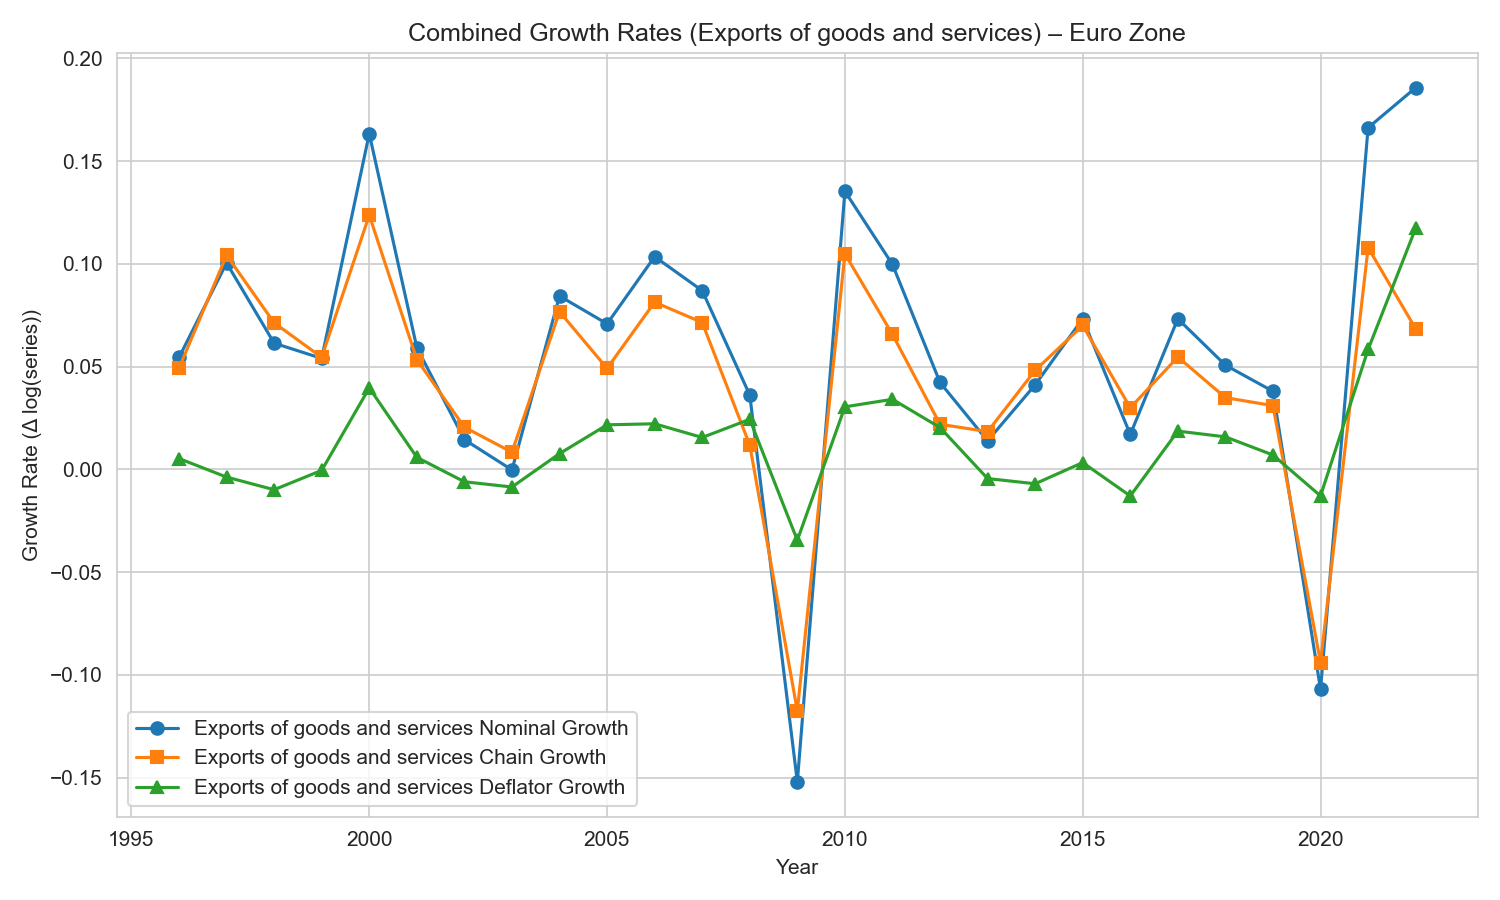
\includegraphics[width=0.8\textwidth]{Exports_of_goods_and_services_combined_growth_Euro.png}
  \vspace{0.5em}

\captionof{figure}{}\end{tcolorbox}
\FloatBarrier

\begin{tcolorbox}[colback=white,colframe=black,title={Εξαγωγές αγαθών και υπηρεσιών: συνδυασμένη ανάπτυξη στην Ελλάδα}]
  \centering
  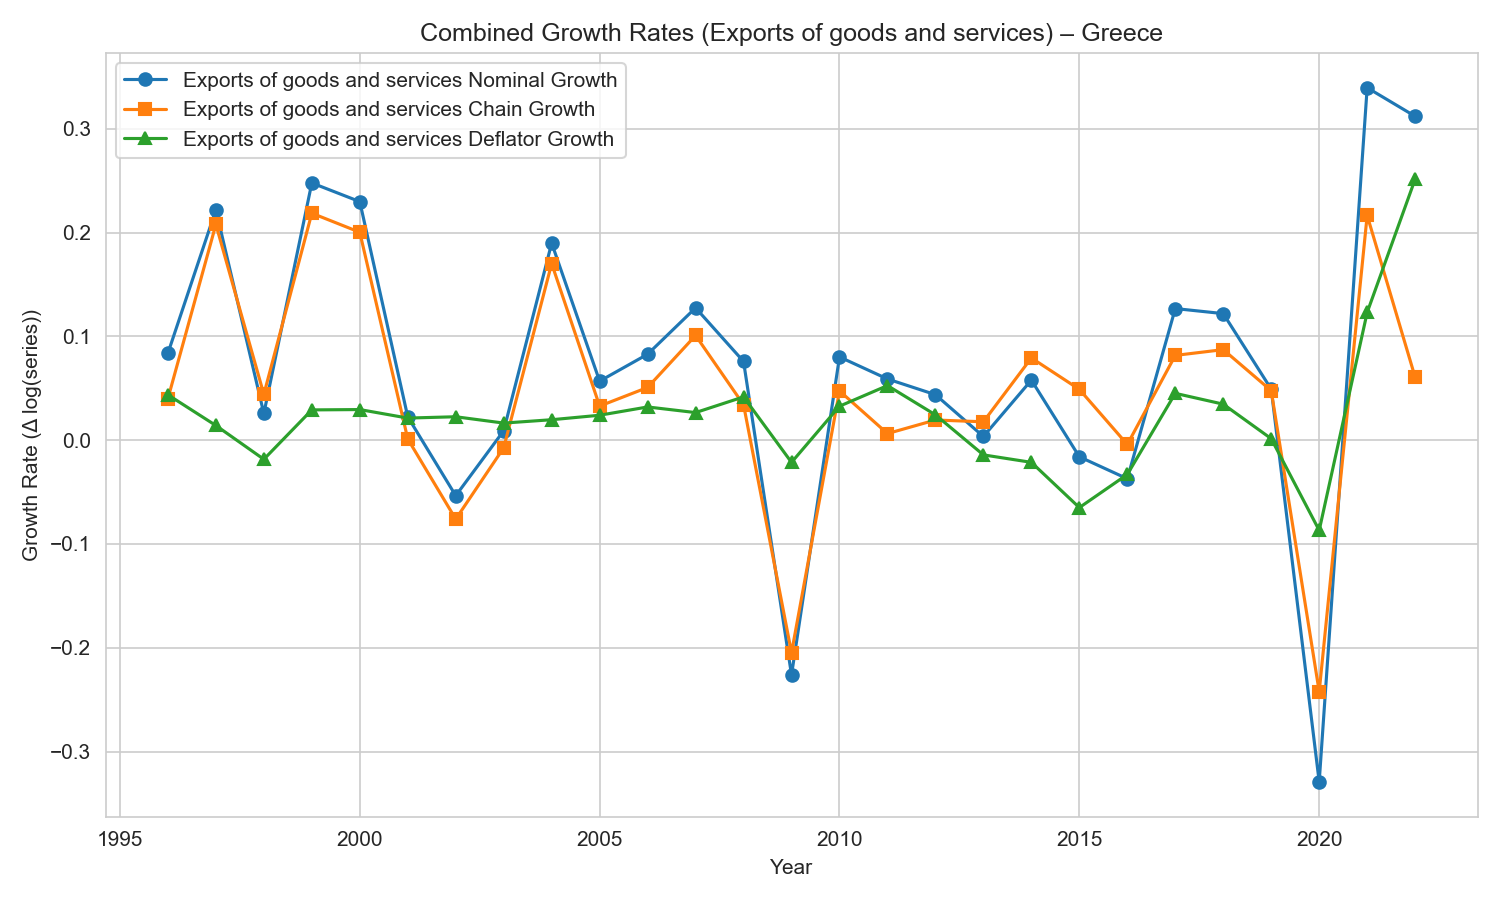
\includegraphics[width=0.8\textwidth]{Exports_of_goods_and_services_combined_growth_Greece.png}
  \vspace{0.5em}

\captionof{figure}{}\end{tcolorbox}
\FloatBarrier

\begin{tcolorbox}[colback=white,colframe=black,title={Εξαγωγές αγαθών και υπηρεσιών: συνδυασμένα επίπεδα}]
  \centering
  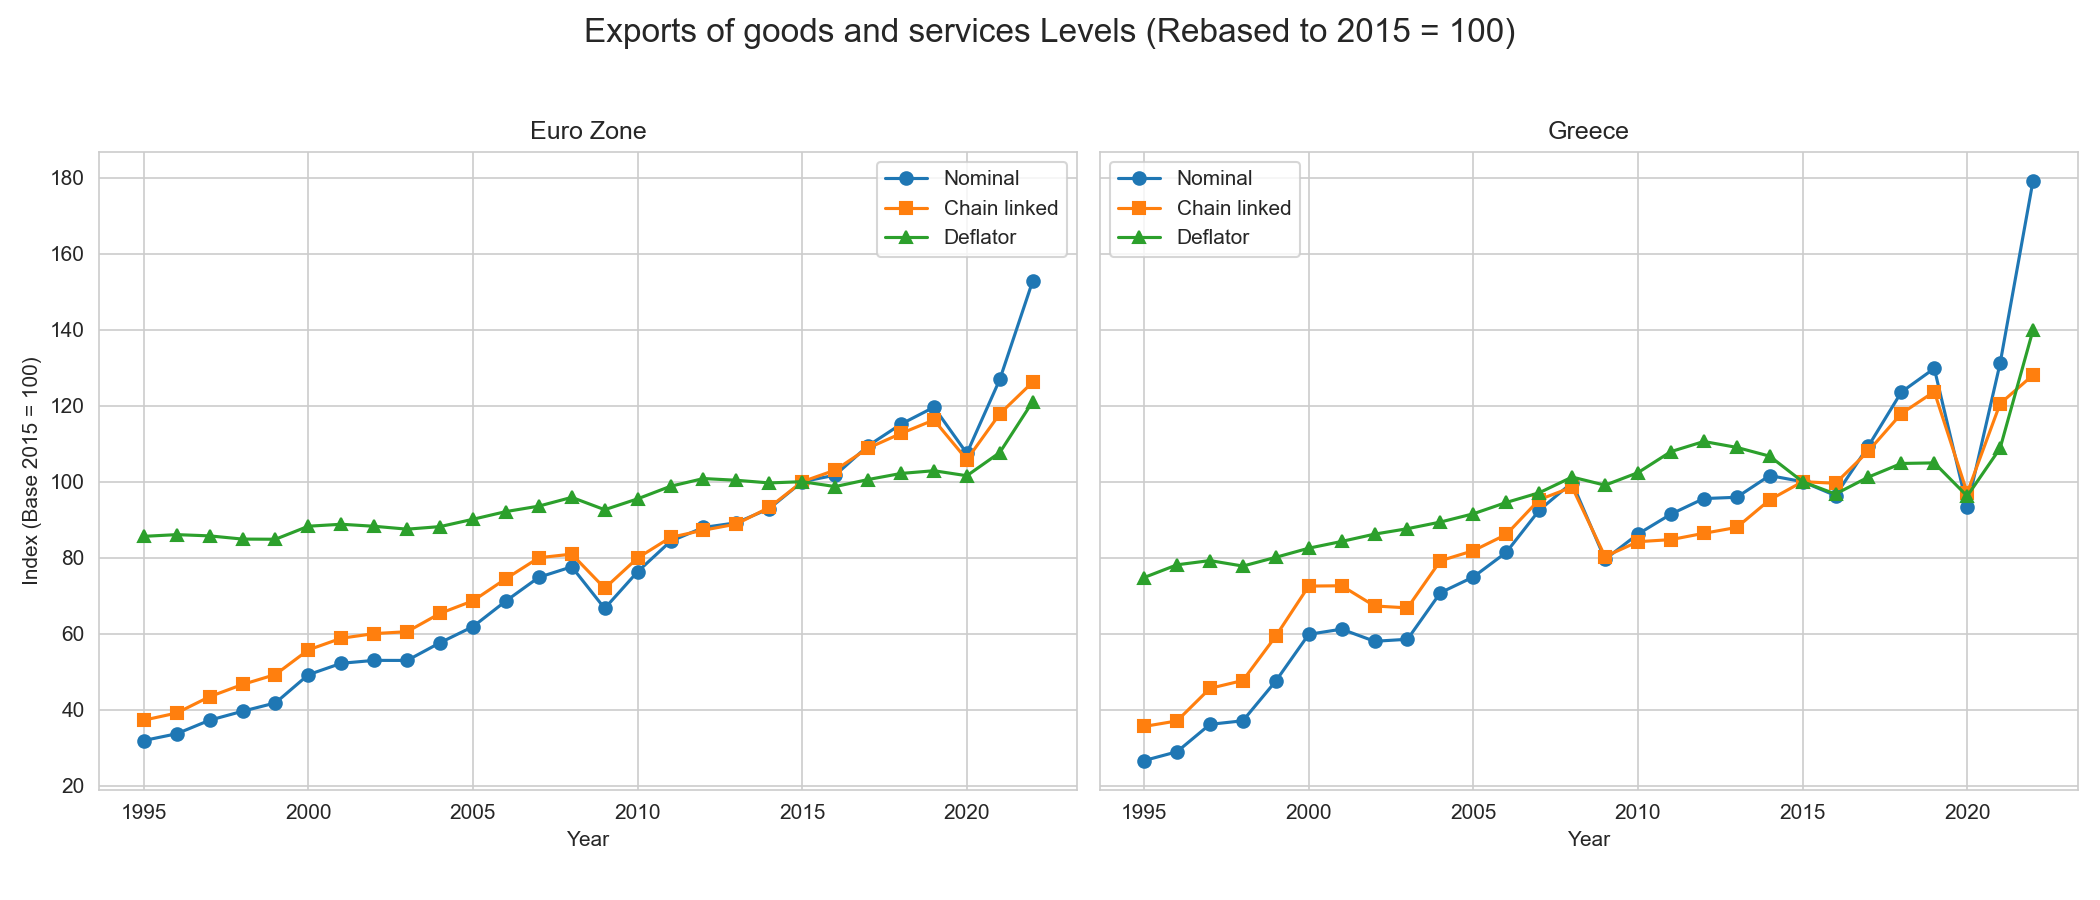
\includegraphics[width=0.8\textwidth]{Exports_of_goods_and_services_combined_levels.png}
  \vspace{0.5em}

\captionof{figure}{}\end{tcolorbox}
\FloatBarrier

\begin{tcolorbox}[colback=white,colframe=black,title={Εξαγωγές αγαθών και υπηρεσιών: αποπληθωριστής}]
  \centering
  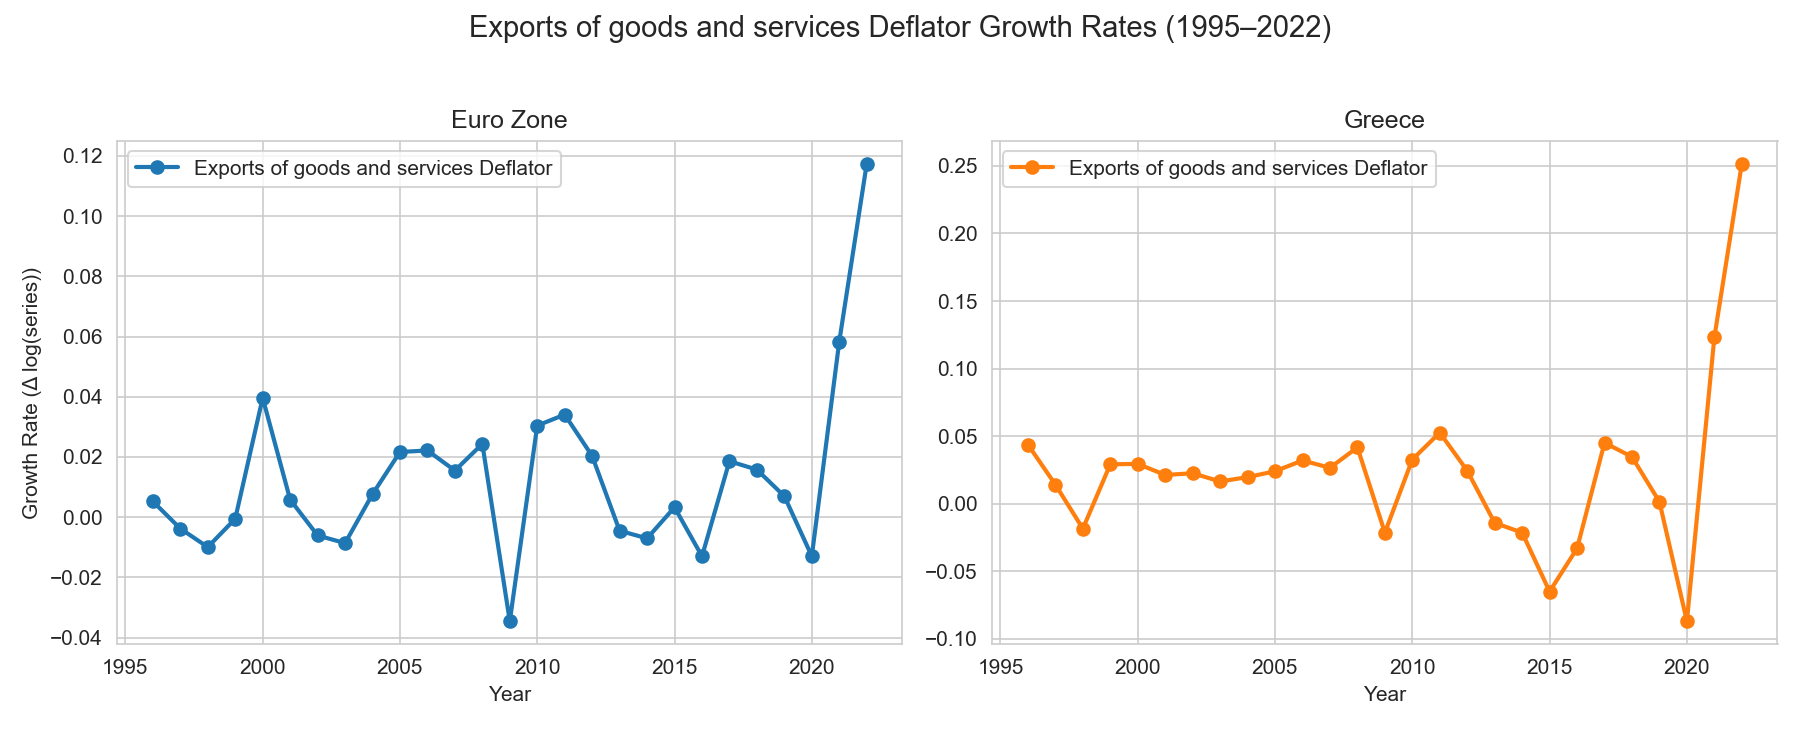
\includegraphics[width=0.8\textwidth]{Exports_of_goods_and_services_deflator_growth.png}
  \vspace{0.5em}

\captionof{figure}{}\end{tcolorbox}
\FloatBarrier

\begin{tcolorbox}[colback=white,colframe=black,title={Εξαγωγές αγαθών και υπηρεσιών: ονομαστική ανάπτυξη}]
  \centering
  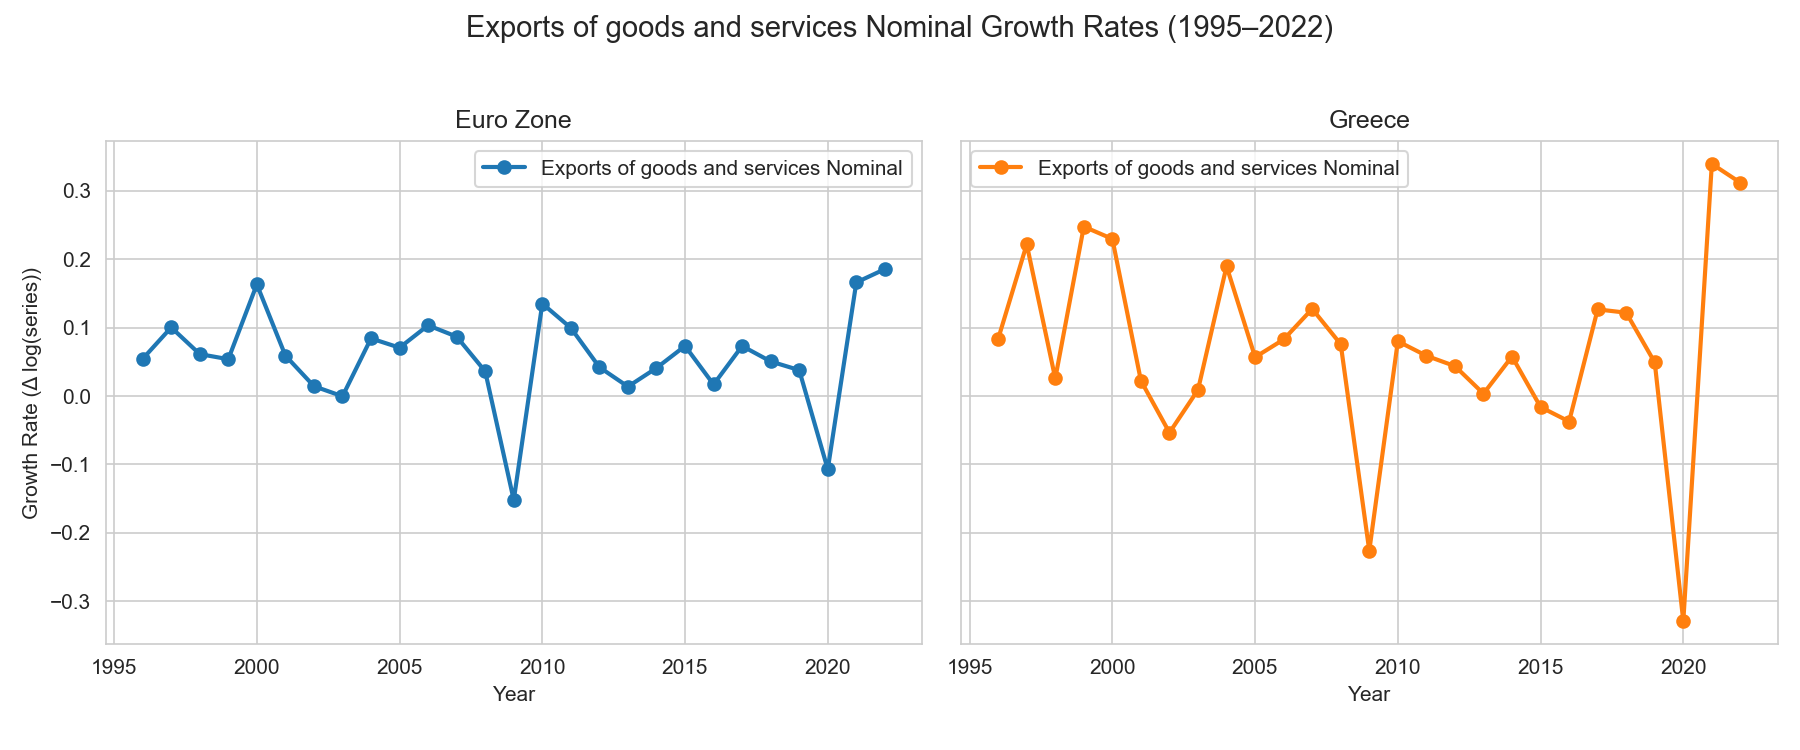
\includegraphics[width=0.8\textwidth]{Exports_of_goods_and_services_nominal_growth.png}
  \vspace{0.5em}

\captionof{figure}{}\end{tcolorbox}
\FloatBarrier

% Παράδειγμα προσαρμογής τίτλων για Τελικές δαπάνες κατανάλωσης
\begin{tcolorbox}[colback=white,colframe=black,title={Τελικές δαπάνες κατανάλωσης: ανάπτυξη αλυσίδας}]
  \centering
  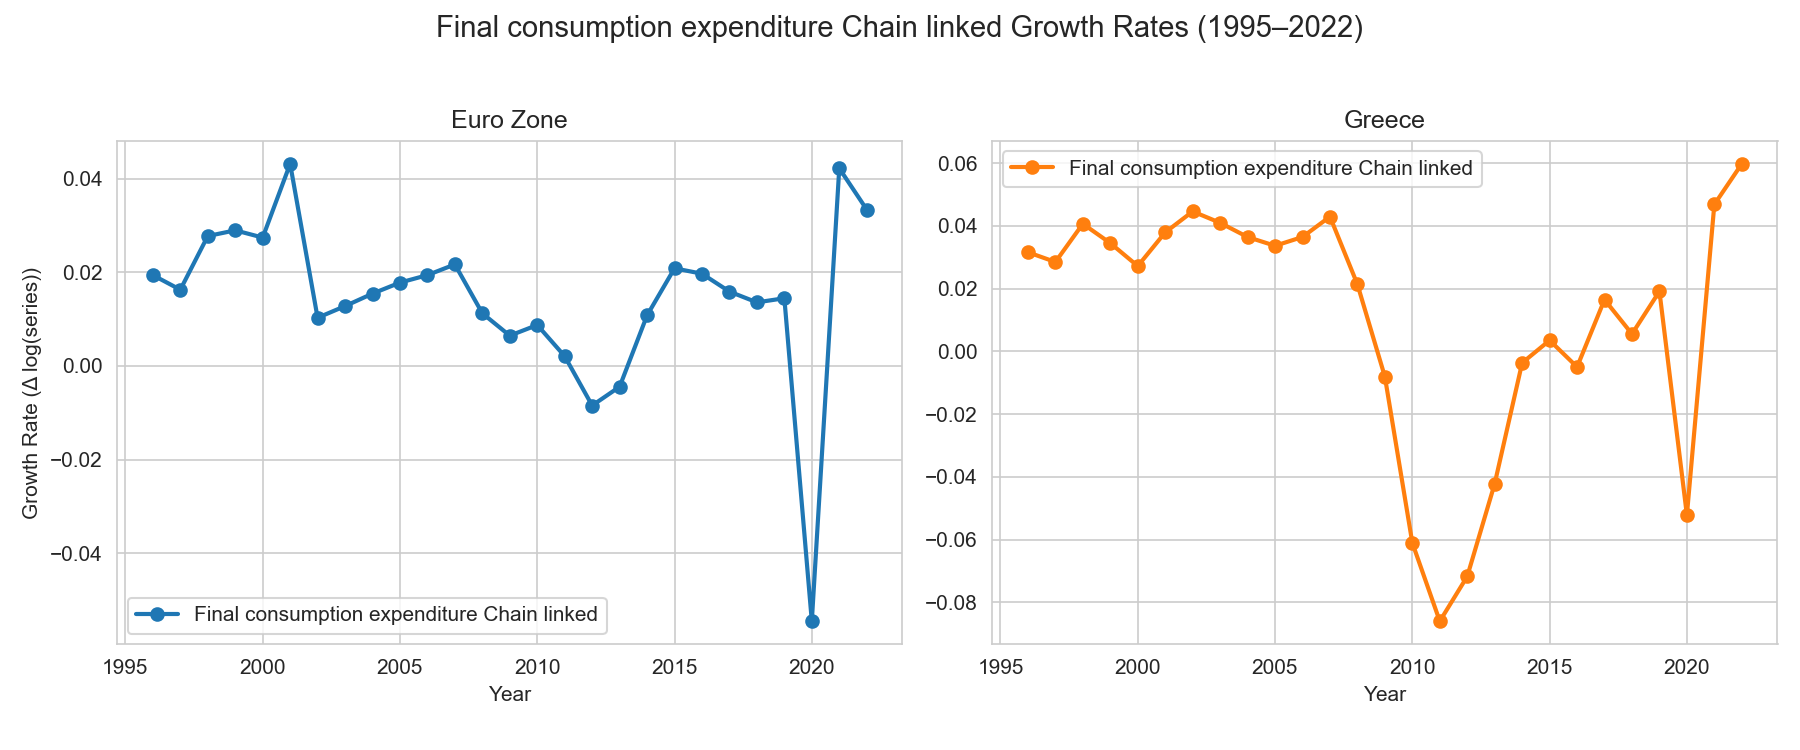
\includegraphics[width=0.8\textwidth]{Final_consumption_expenditure_chain_growth.png}
  \vspace{0.5em}

\captionof{figure}{}\end{tcolorbox}
\FloatBarrier

\begin{tcolorbox}[colback=white,colframe=black,title={Τελικές δαπάνες κατανάλωσης: συνδυασμένη ανάπτυξη στην Ευρωζώνη}]
  \centering
  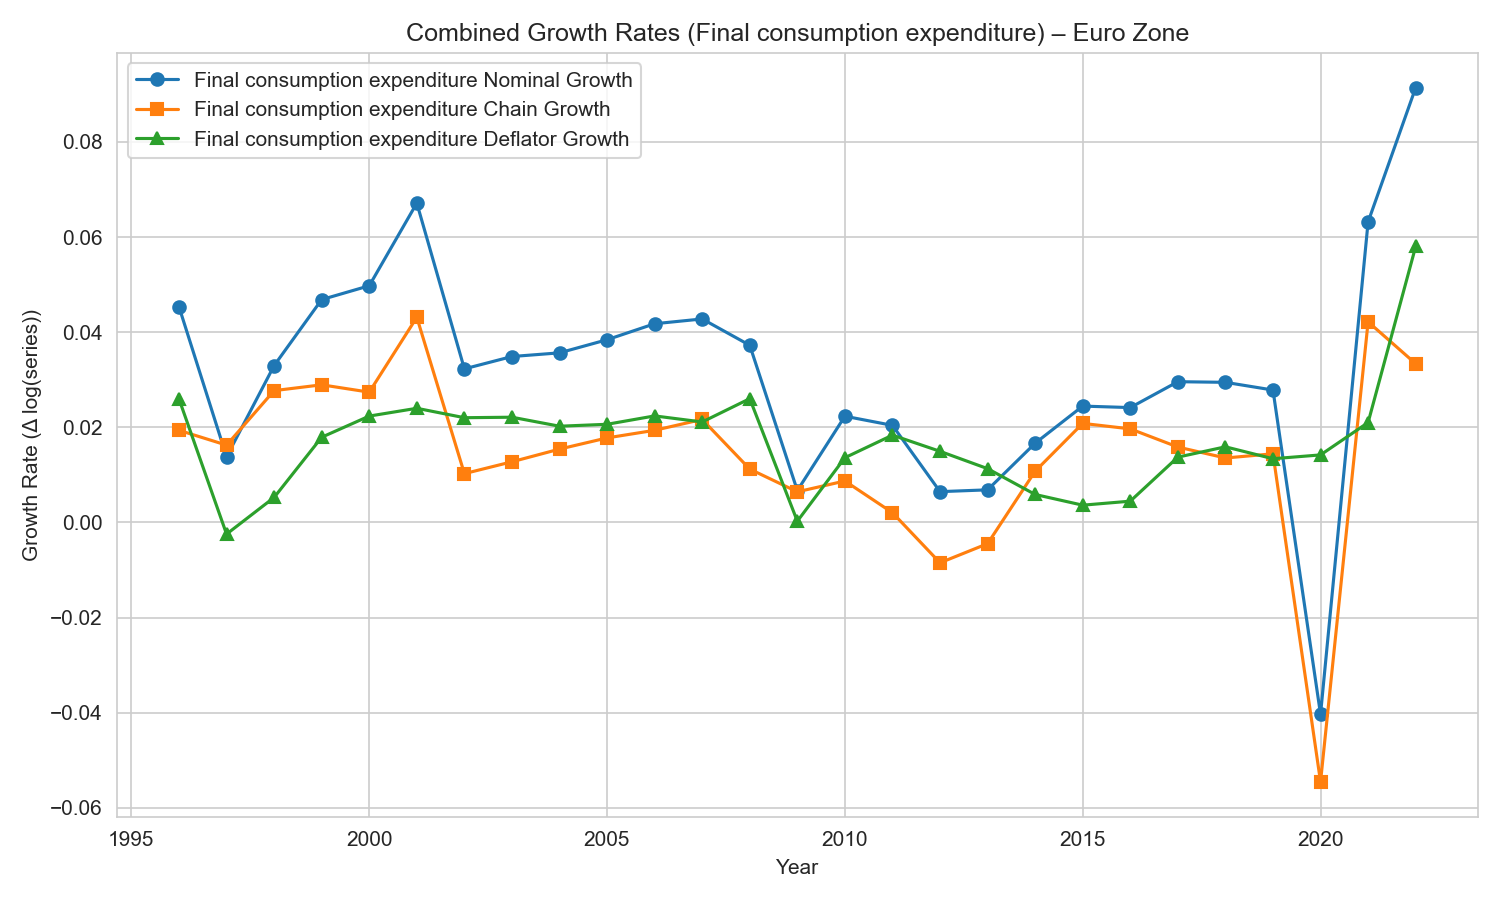
\includegraphics[width=0.8\textwidth]{Final_consumption_expenditure_combined_growth_Euro.png}
  \vspace{0.5em}

\captionof{figure}{}\end{tcolorbox}
\FloatBarrier

\begin{tcolorbox}[colback=white,colframe=black,title={Τελικές δαπάνες κατανάλωσης: συνδυασμένη ανάπτυξη στην Ελλάδα}]
  \centering
  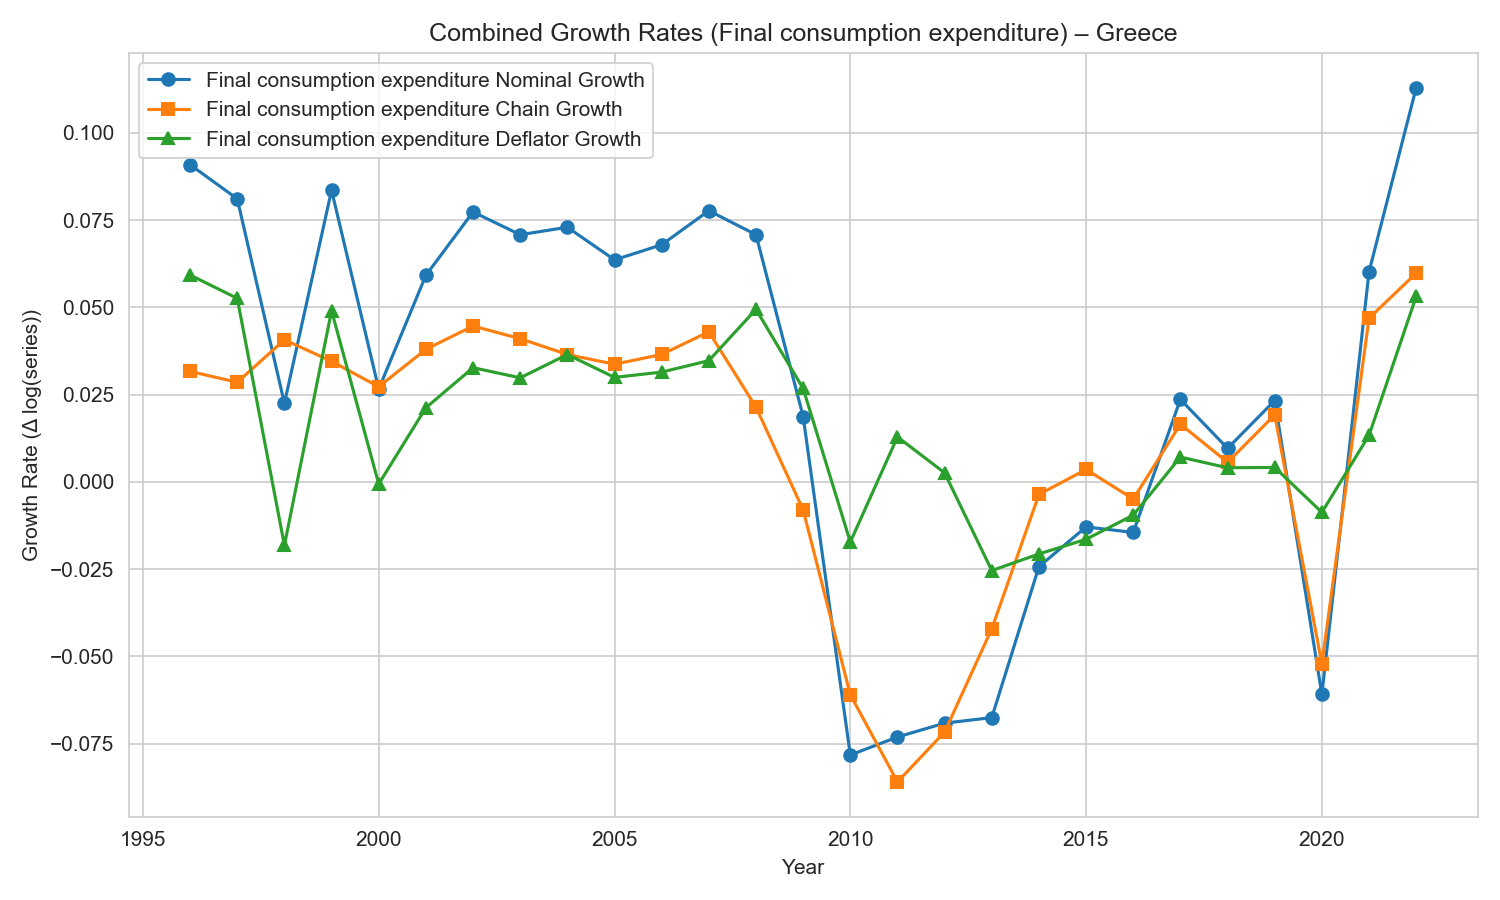
\includegraphics[width=0.8\textwidth]{Final_consumption_expenditure_combined_growth_Greece.png}
  \vspace{0.5em}

\captionof{figure}{}\end{tcolorbox}
\FloatBarrier

\begin{tcolorbox}[colback=white,colframe=black,title={Τελικές δαπάνες κατανάλωσης: συνδυασμένα επίπεδα}]
  \centering
  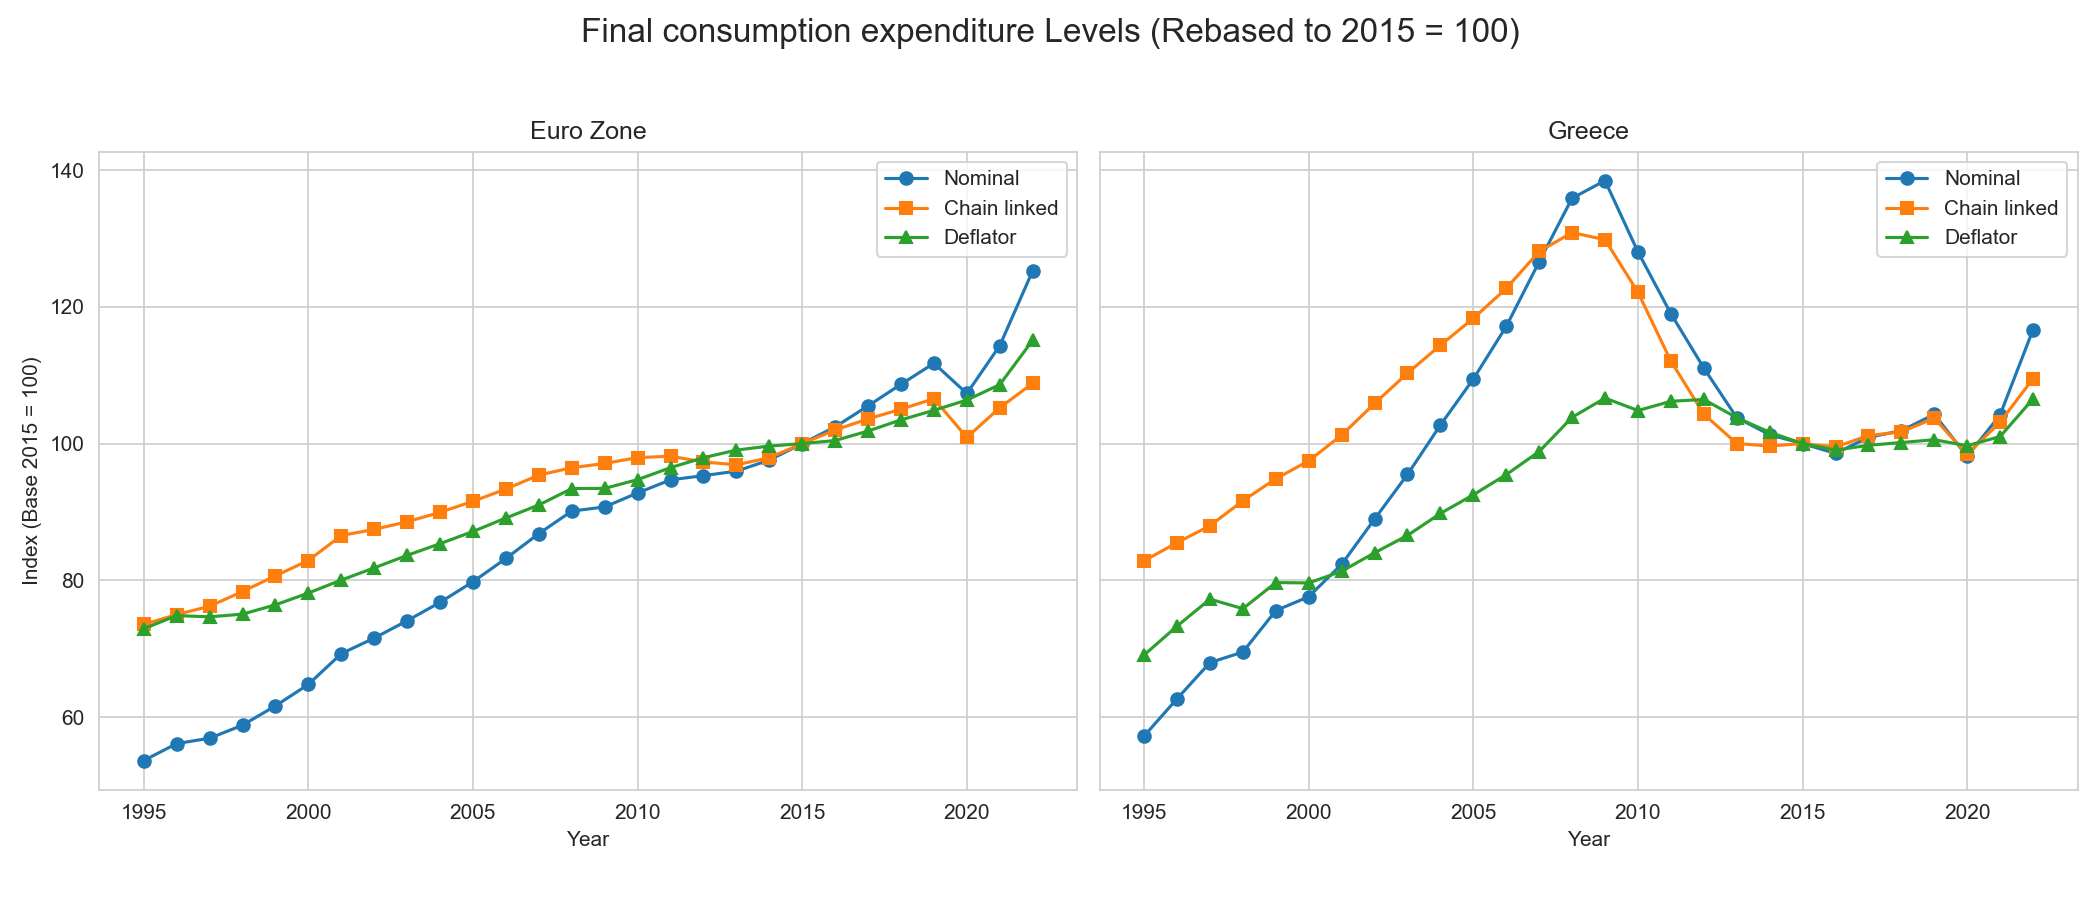
\includegraphics[width=0.8\textwidth]{Final_consumption_expenditure_combined_levels.png}
  \vspace{0.5em}

\captionof{figure}{}\end{tcolorbox}
\FloatBarrier

\begin{tcolorbox}[colback=white,colframe=black,title={Τελικές δαπάνες κατανάλωσης: αποπληθωριστής}]
  \centering
  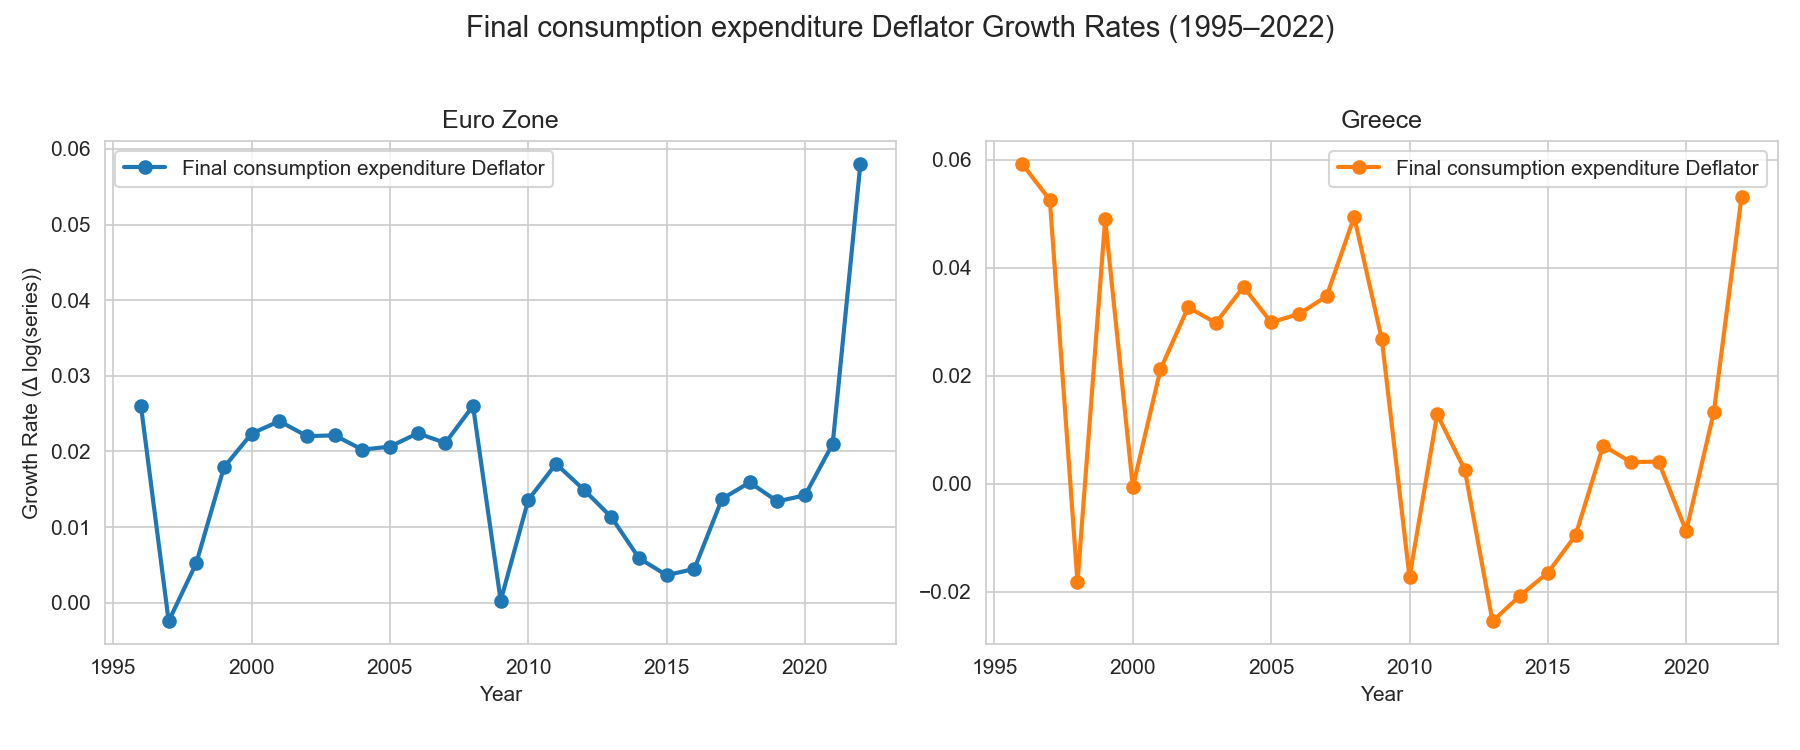
\includegraphics[width=0.8\textwidth]{Final_consumption_expenditure_deflator_growth.png}
  \vspace{0.5em}

\captionof{figure}{}\end{tcolorbox}
\FloatBarrier

\begin{tcolorbox}[colback=white,colframe=black,title={Τελικές δαπάνες κατανάλωσης: ονομαστική ανάπτυξη}]
  \centering
  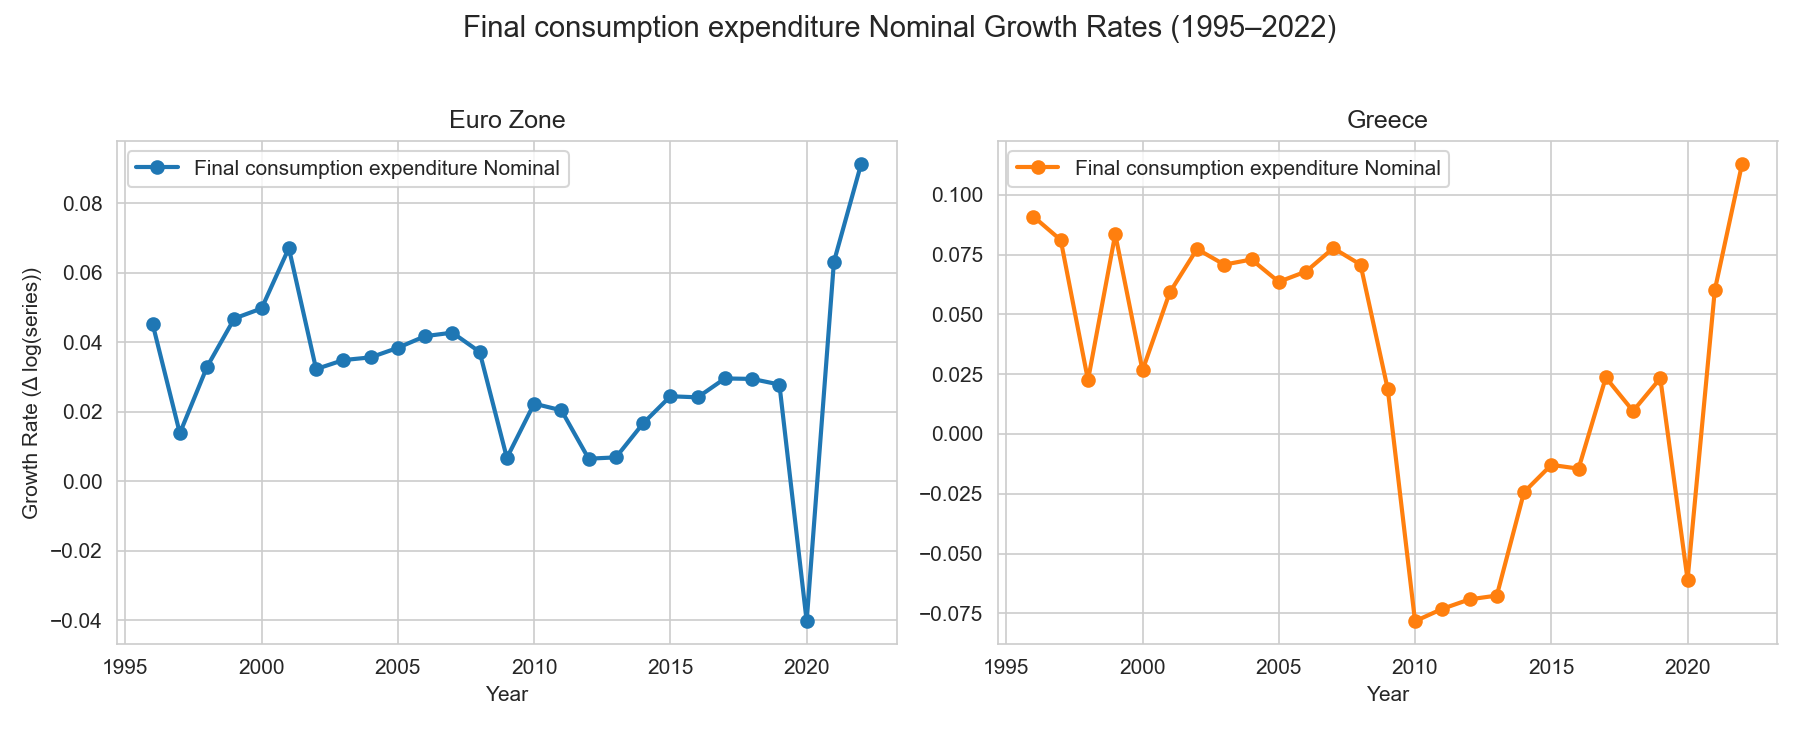
\includegraphics[width=0.8\textwidth]{Final_consumption_expenditure_nominal_growth.png}
  \vspace{0.5em}

\captionof{figure}{}\end{tcolorbox}
\FloatBarrier

% Παρομοίως για τις υπόλοιπες μεταβλητές (γενική κυβέρνηση, νοικοκυριά κ.λπ.)
% Τίτλοι όπως:
% «Τελικές δαπάνες κατανάλωσης γενικής κυβέρνησης: ανάπτυξη αλυσίδας»
% «Τελικές δαπάνες κατανάλωσης νοικοκυριών: συνδυασμένη ανάπτυξη στην Ελλάδα»
% κ.ο.κ.

\begin{tcolorbox}[colback=white,colframe=black,title={Τελικές δαπάνες κατανάλωσης γενικής κυβέρνησης: ανάπτυξη αλυσίδας}]
  \centering
  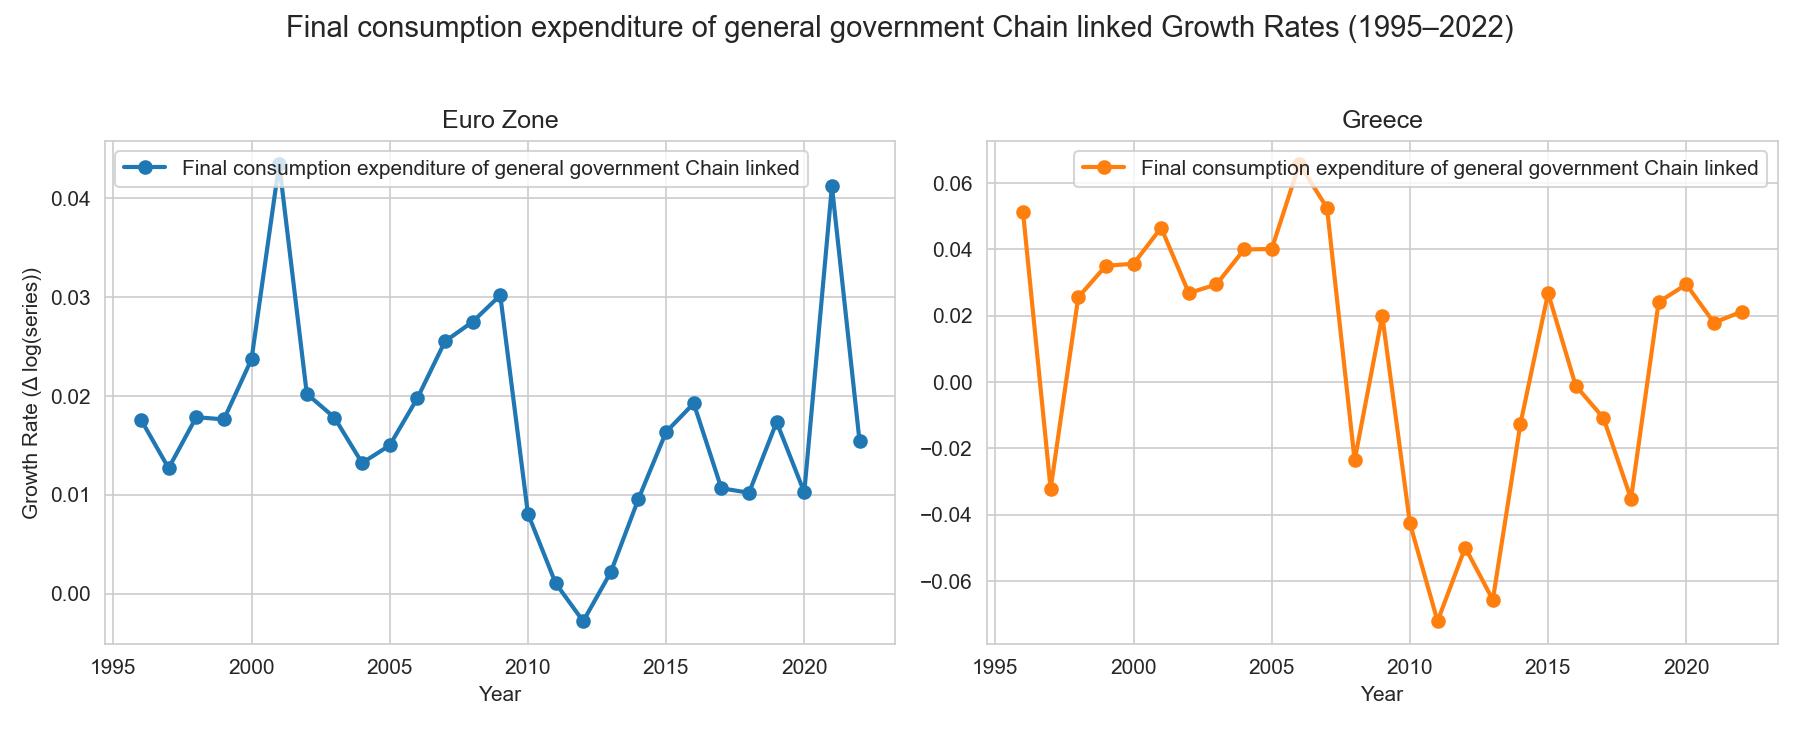
\includegraphics[width=0.8\textwidth]{Final_consumption_expenditure_of_general_government_chain_growth.png}
  \vspace{0.5em}

\captionof{figure}{}\end{tcolorbox}
\FloatBarrier

\begin{tcolorbox}[colback=white,colframe=black,title={Τελικές δαπάνες κατανάλωσης γενικής κυβέρνησης: συνδυασμένη ανάπτυξη στην Ευρωζώνη}]
  \centering
  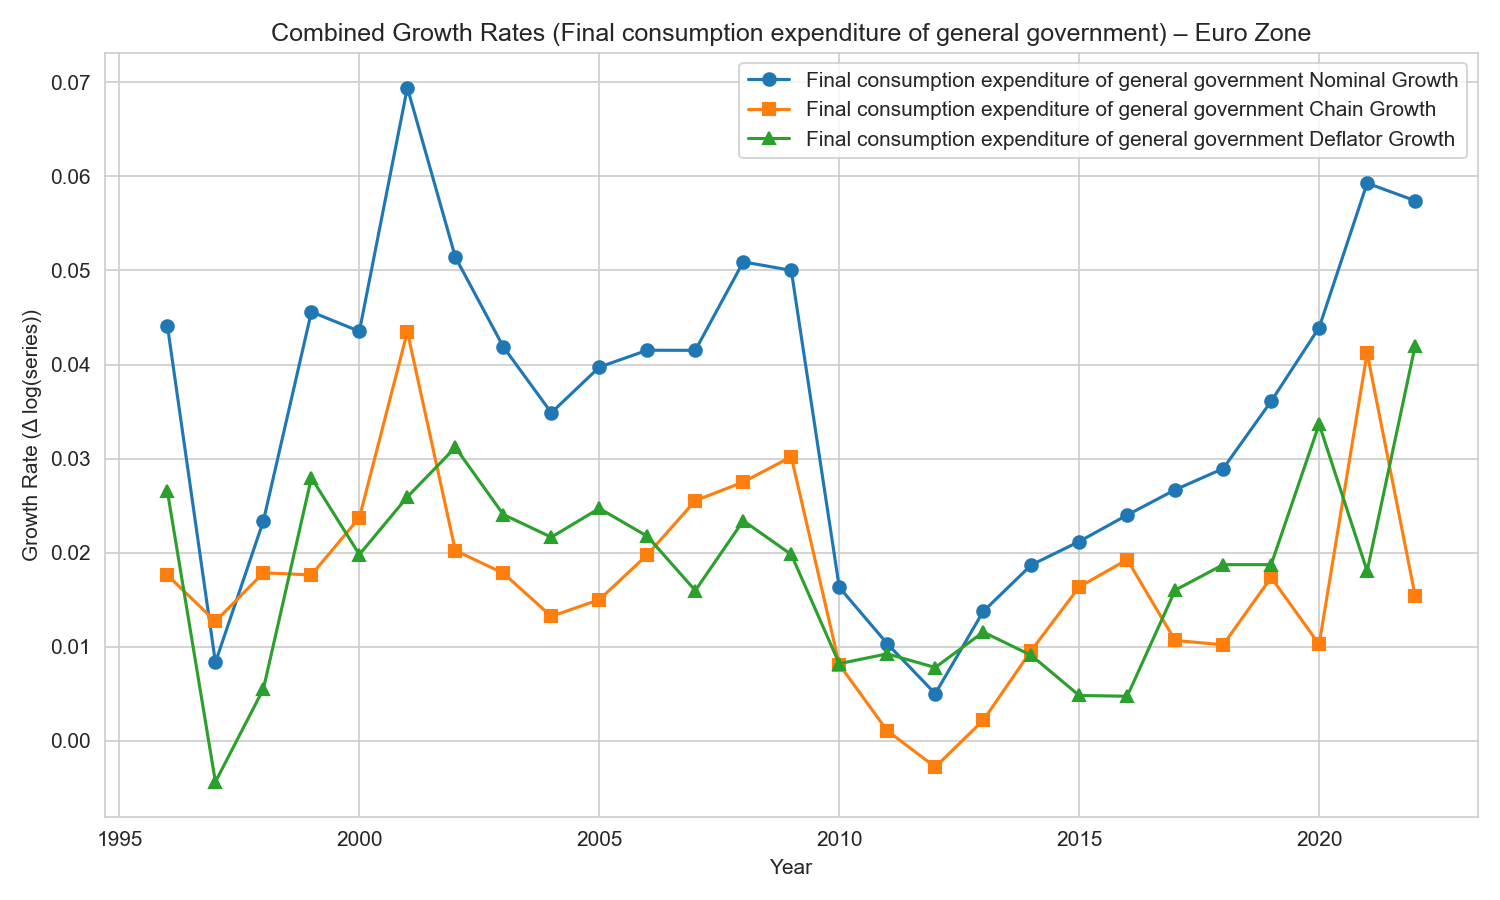
\includegraphics[width=0.8\textwidth]{Final_consumption_expenditure_of_general_government_combined_growth_Euro.png}
  \vspace{0.5em}

\captionof{figure}{}\end{tcolorbox}
\FloatBarrier

\begin{tcolorbox}[colback=white,colframe=black,title={Τελικές δαπάνες κατανάλωσης γενικής κυβέρνησης: συνδυασμένη ανάπτυξη στην Ελλάδα}]
  \centering
  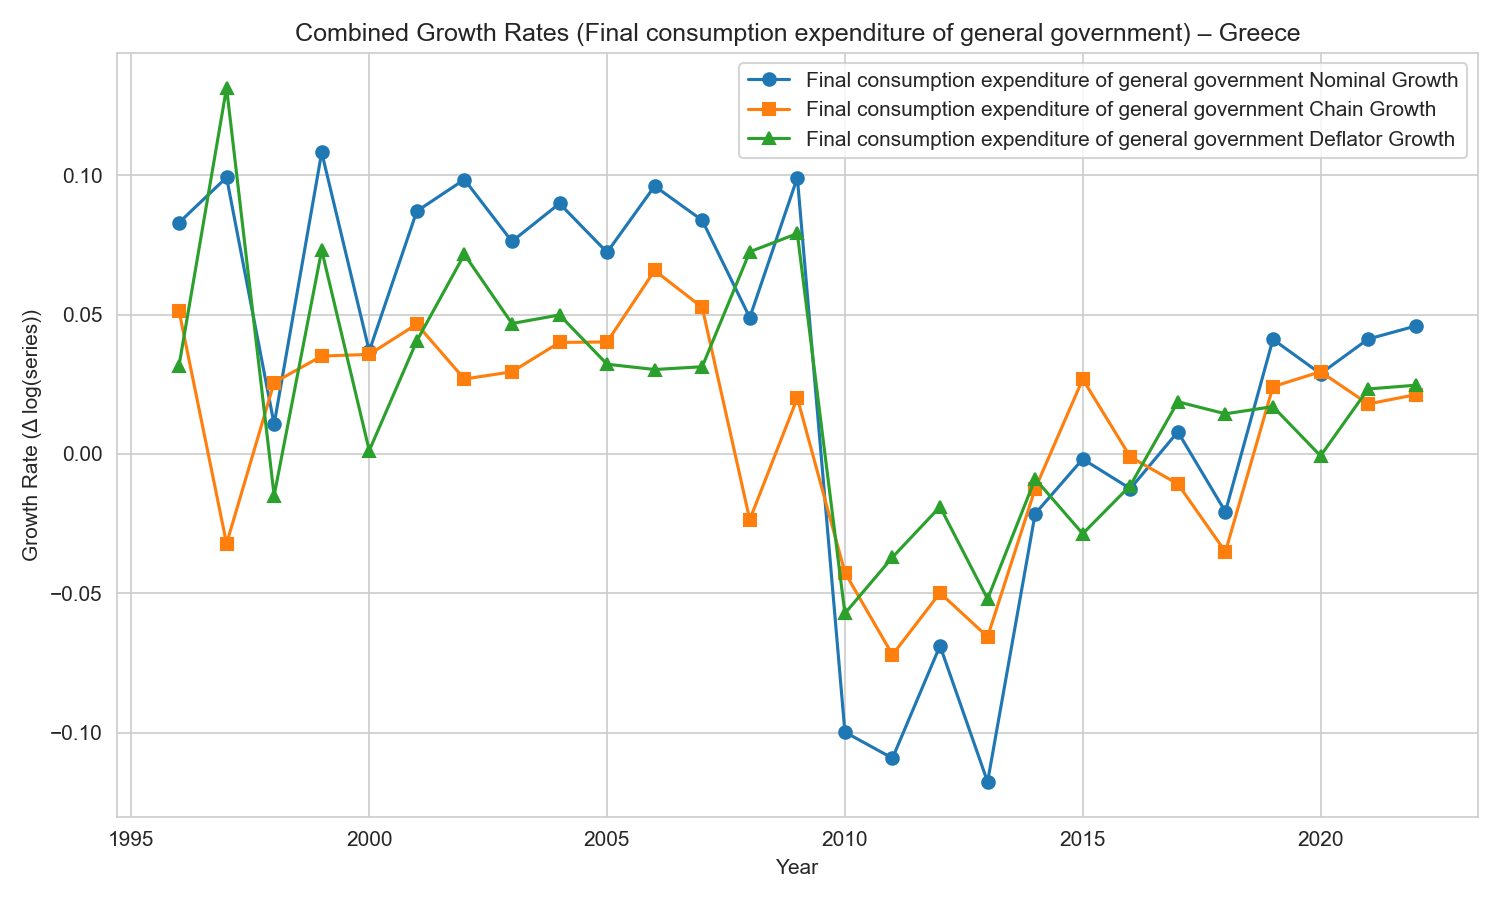
\includegraphics[width=0.8\textwidth]{Final_consumption_expenditure_of_general_government_combined_growth_Greece.png}
  \vspace{0.5em}

\captionof{figure}{}\end{tcolorbox}
\FloatBarrier

\begin{tcolorbox}[colback=white,colframe=black,title={Τελικές δαπάνες κατανάλωσης γενικής κυβέρνησης: συνδυασμένα επίπεδα}]
  \centering
  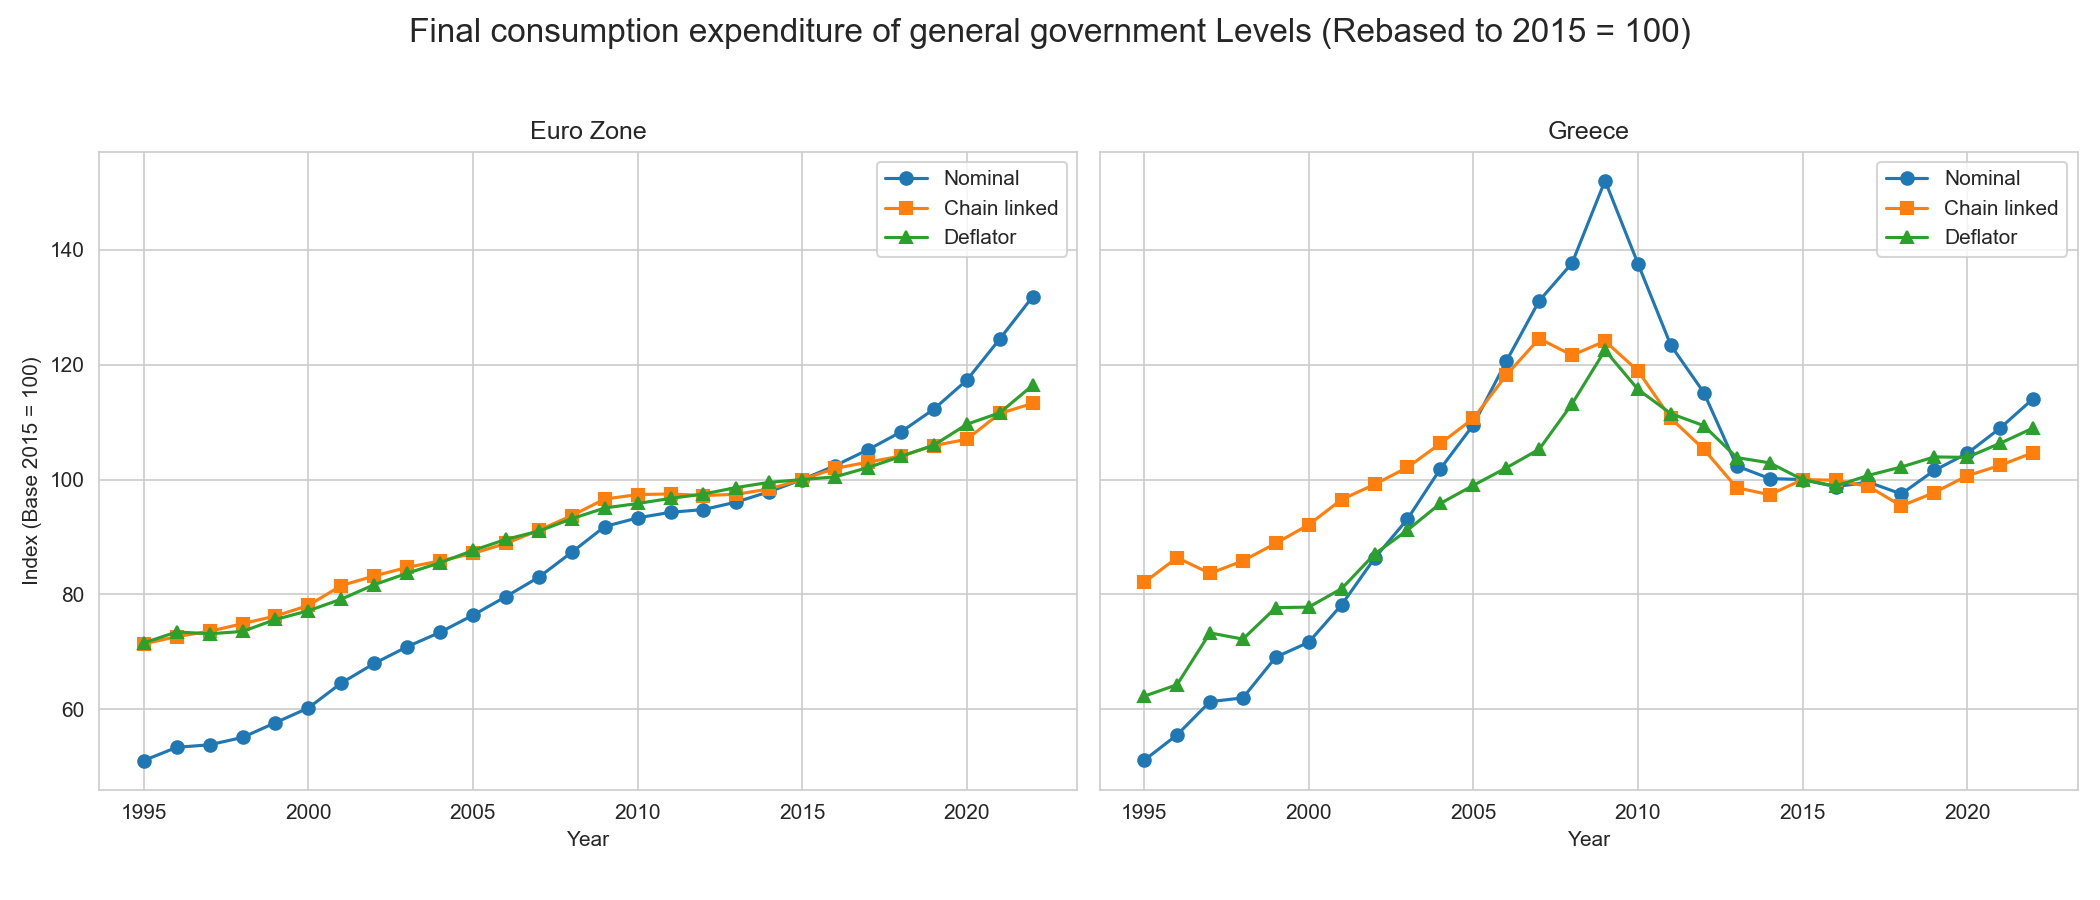
\includegraphics[width=0.8\textwidth]{Final_consumption_expenditure_of_general_government_combined_levels.png}
  \vspace{0.5em}

\captionof{figure}{}\end{tcolorbox}
\FloatBarrier

\begin{tcolorbox}[colback=white,colframe=black,title={Τελικές δαπάνες κατανάλωσης γενικής κυβέρνησης: αποπληθωριστής}]
  \centering
  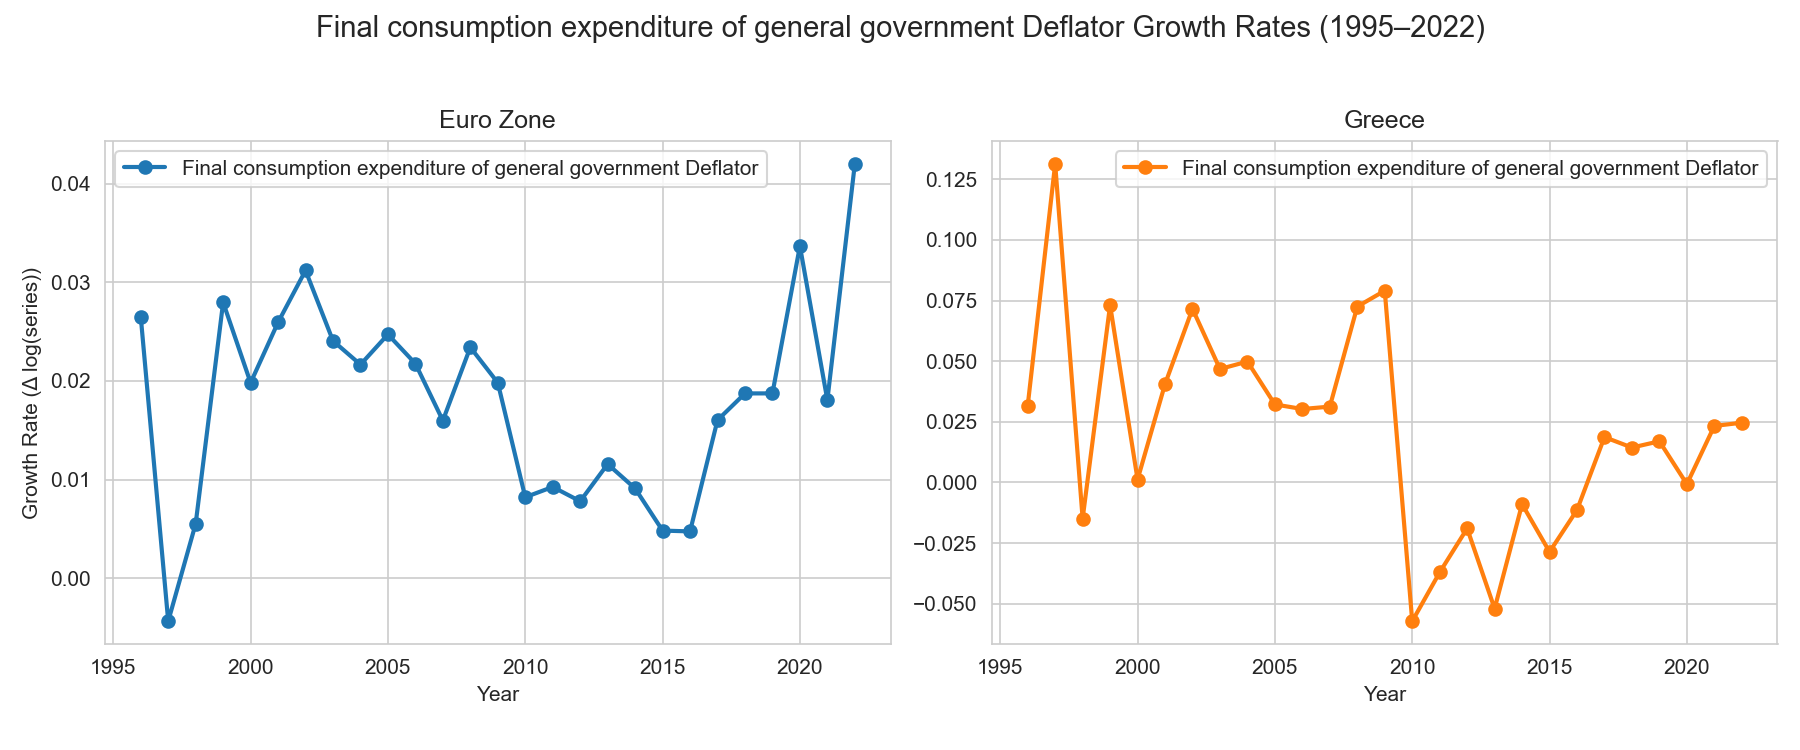
\includegraphics[width=0.8\textwidth]{Final_consumption_expenditure_of_general_government_deflator_growth.png}
  \vspace{0.5em}

\captionof{figure}{}\end{tcolorbox}
\FloatBarrier

\begin{tcolorbox}[colback=white,colframe=black,title={Τελικές δαπάνες κατανάλωσης γενικής κυβέρνησης: ονομαστική ανάπτυξη}]
  \centering
  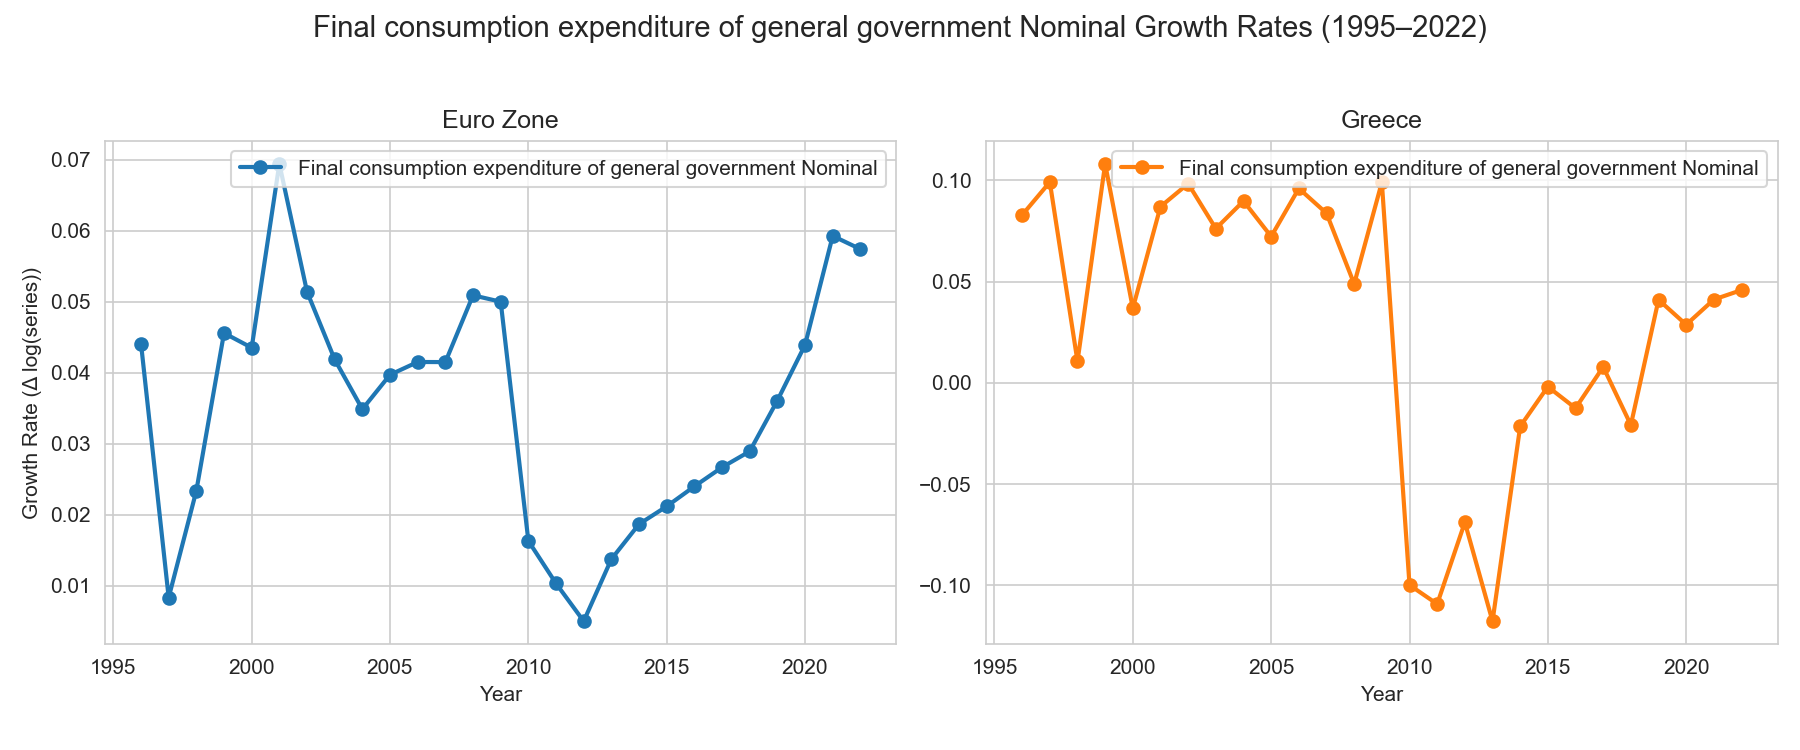
\includegraphics[width=0.8\textwidth]{Final_consumption_expenditure_of_general_government_nominal_growth.png}
  \vspace{0.5em}

\captionof{figure}{}\end{tcolorbox}
\FloatBarrier

% Παράδειγμα για νοικοκυριά
\begin{tcolorbox}[colback=white,colframe=black,title={Τελικές δαπάνες κατανάλωσης νοικοκυριών: ανάπτυξη αλυσίδας}]
  \centering
  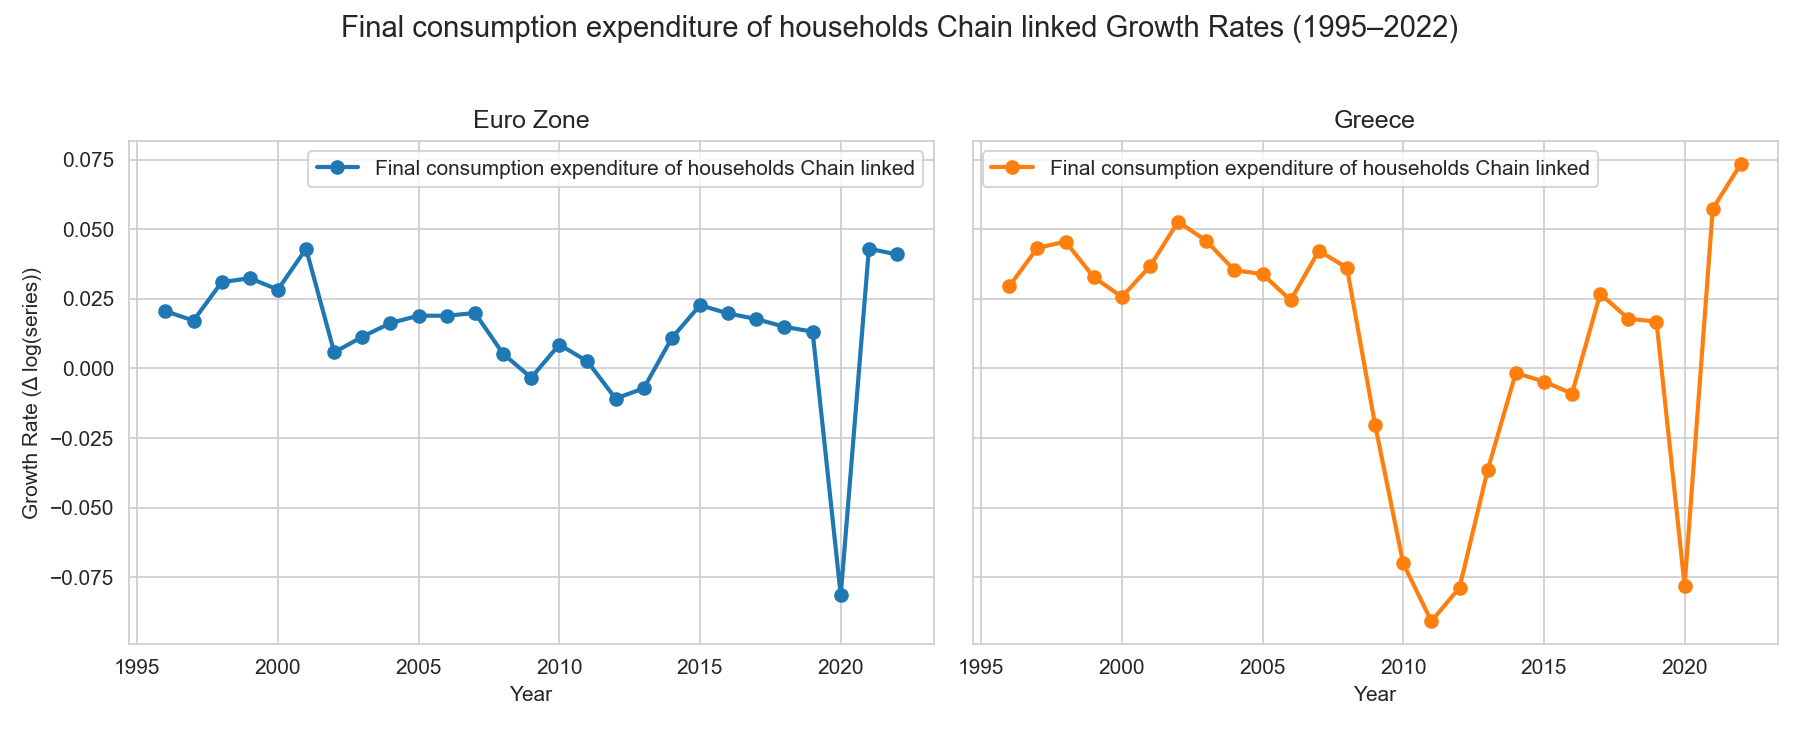
\includegraphics[width=0.8\textwidth]{Final_consumption_expenditure_of_households_chain_growth.png}
  \vspace{0.5em}

\captionof{figure}{}\end{tcolorbox}
\FloatBarrier

\begin{tcolorbox}[colback=white,colframe=black,title={Τελικές δαπάνες κατανάλωσης νοικοκυριών: συνδυασμένη ανάπτυξη στην Ευρωζώνη}]
  \centering
  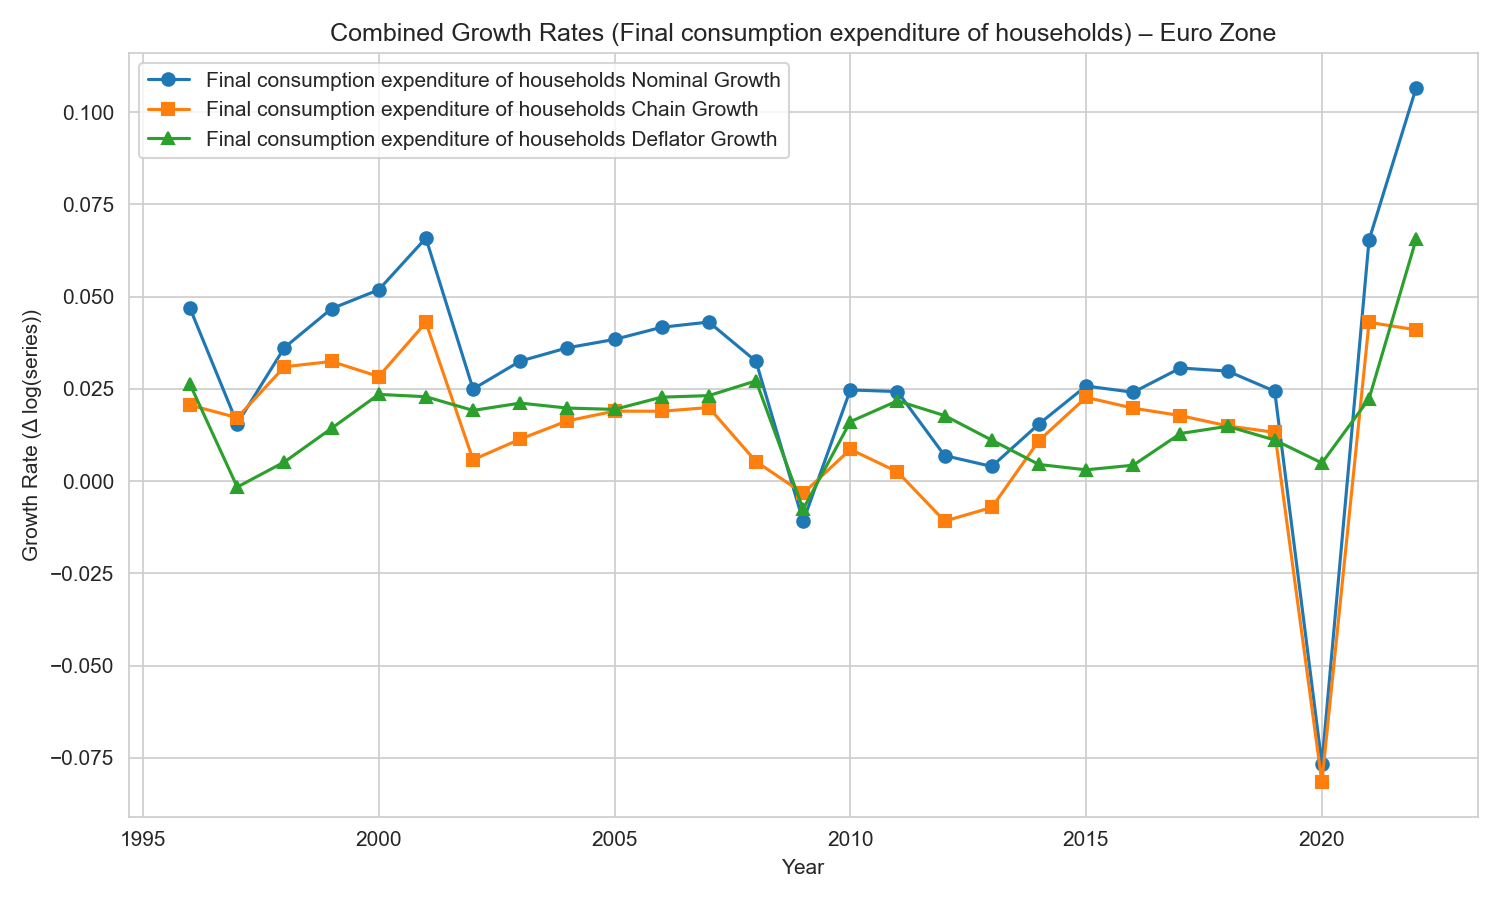
\includegraphics[width=0.8\textwidth]{Final_consumption_expenditure_of_households_combined_growth_Euro.png}
  \vspace{0.5em}

\captionof{figure}{}\end{tcolorbox}
\FloatBarrier

\begin{tcolorbox}[colback=white,colframe=black,title={Τελικές δαπάνες κατανάλωσης νοικοκυριών: συνδυασμένη ανάπτυξη στην Ελλάδα}]
  \centering
  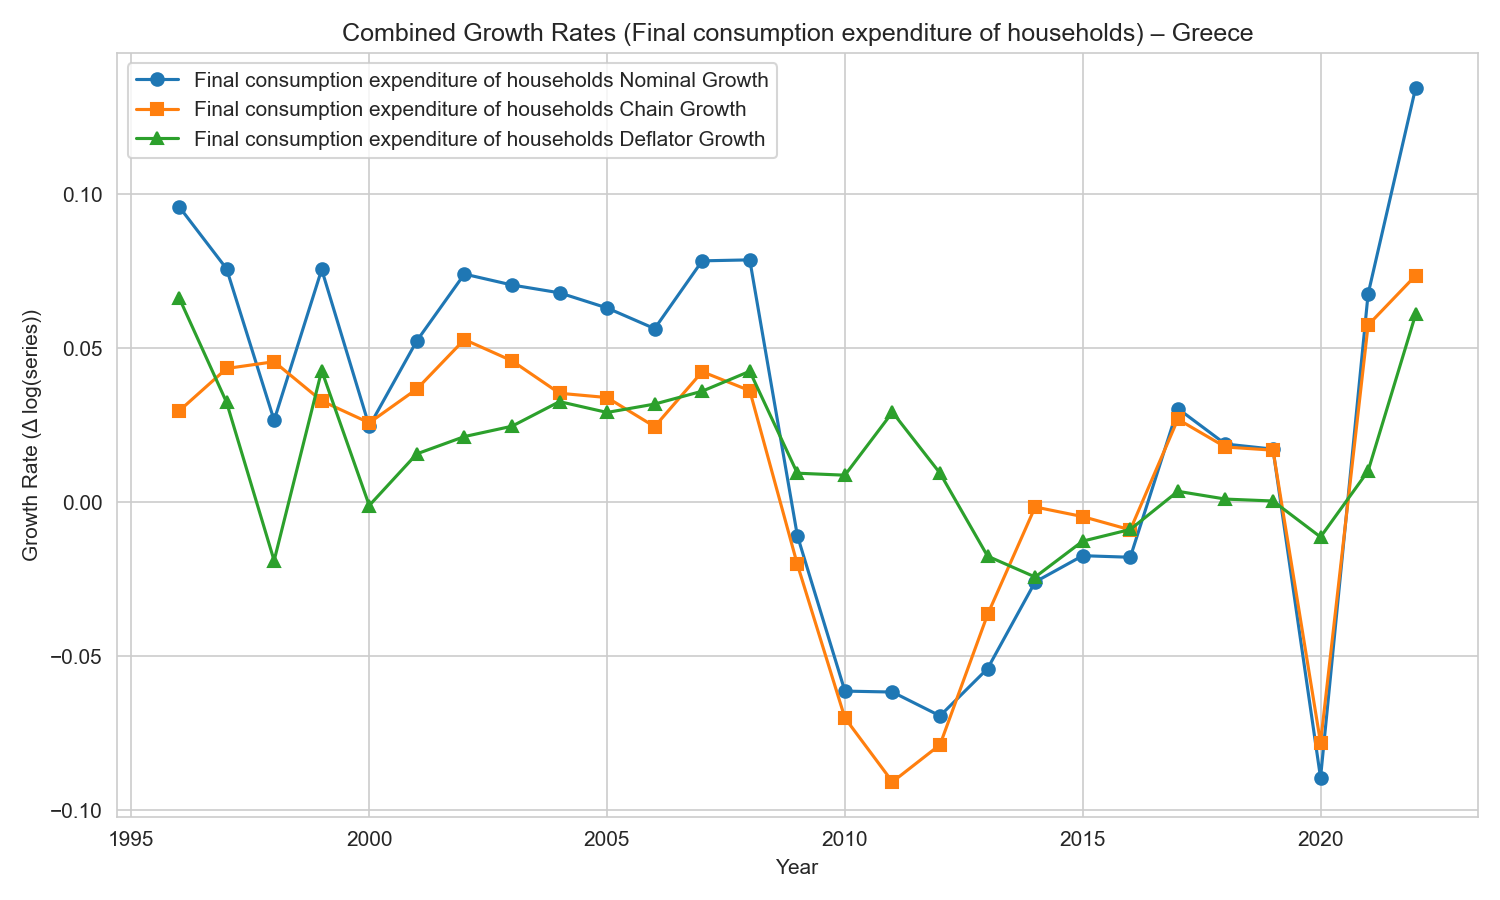
\includegraphics[width=0.8\textwidth]{Final_consumption_expenditure_of_households_combined_growth_Greece.png}
  \vspace{0.5em}

\captionof{figure}{}\end{tcolorbox}
\FloatBarrier

\begin{tcolorbox}[colback=white,colframe=black,title={Τελικές δαπάνες κατανάλωσης νοικοκυριών: συνδυασμένα επίπεδα}]
  \centering
  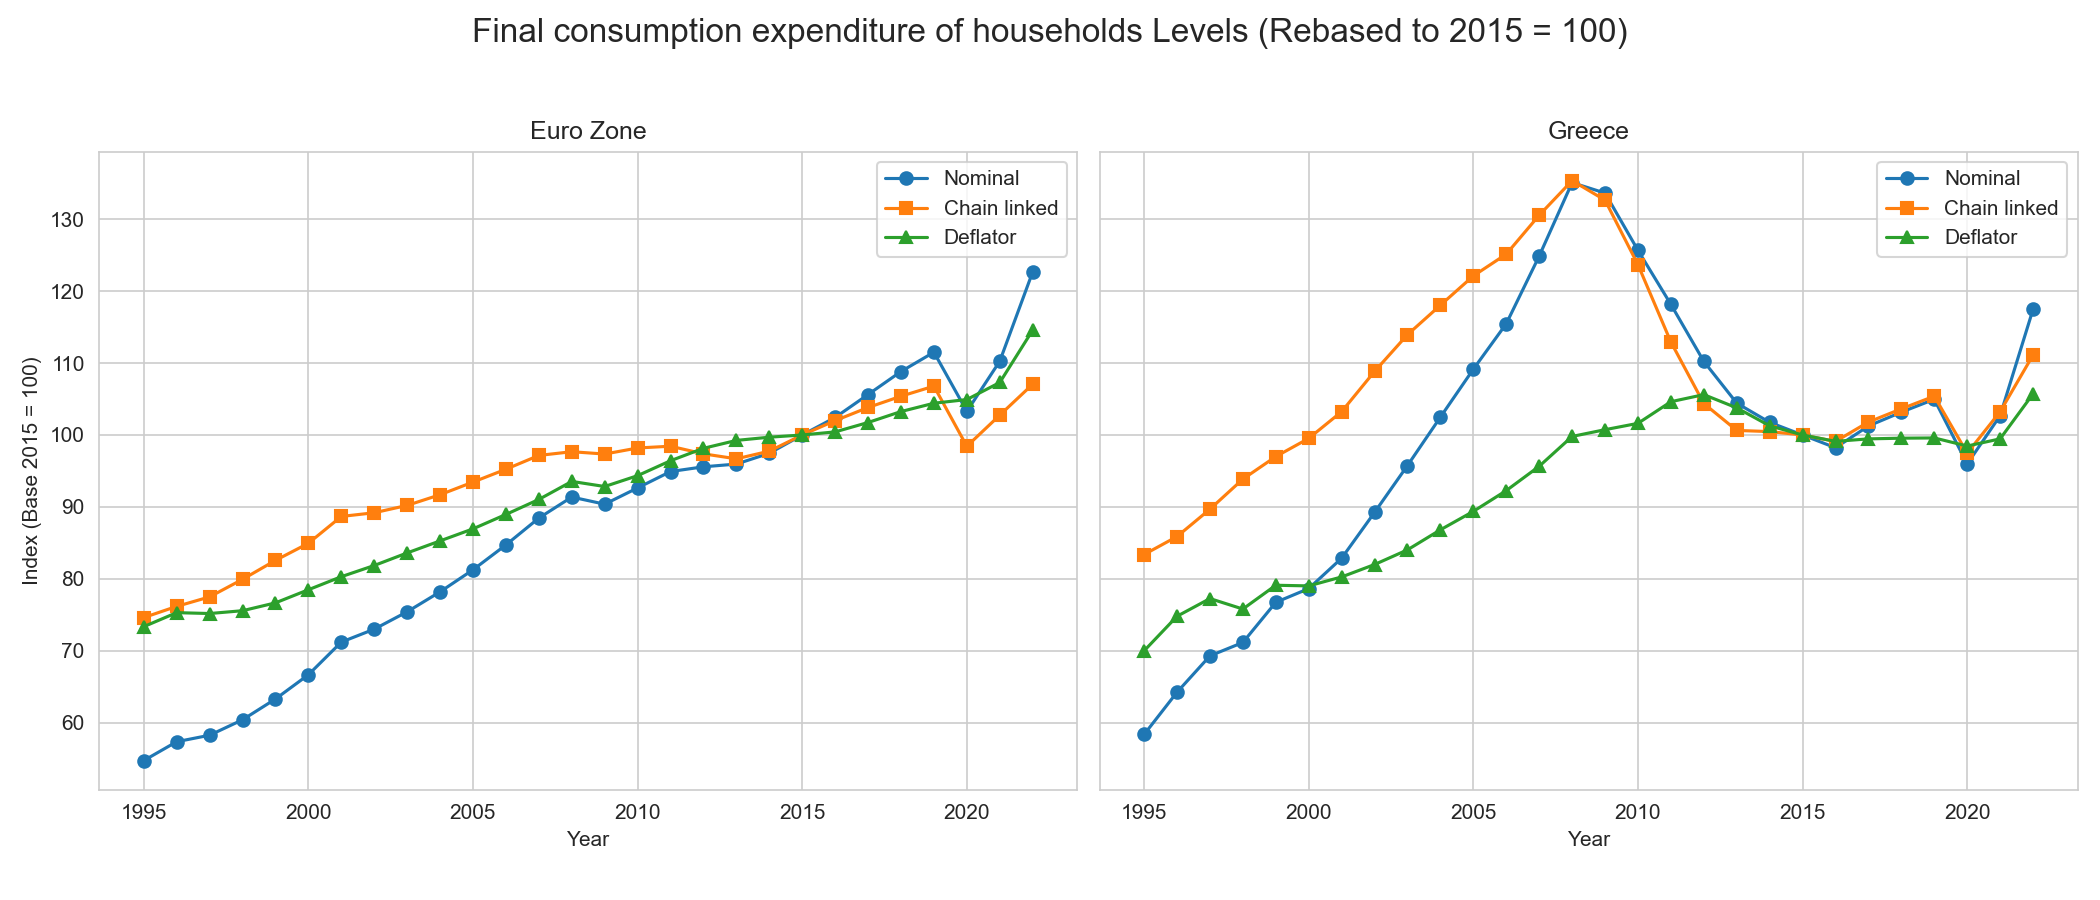
\includegraphics[width=0.8\textwidth]{Final_consumption_expenditure_of_households_combined_levels.png}
  \vspace{0.5em}

\captionof{figure}{}\end{tcolorbox}
\FloatBarrier

\begin{tcolorbox}[colback=white,colframe=black,title={Τελικές δαπάνες κατανάλωσης νοικοκυριών: αποπληθωριστής}]
  \centering
  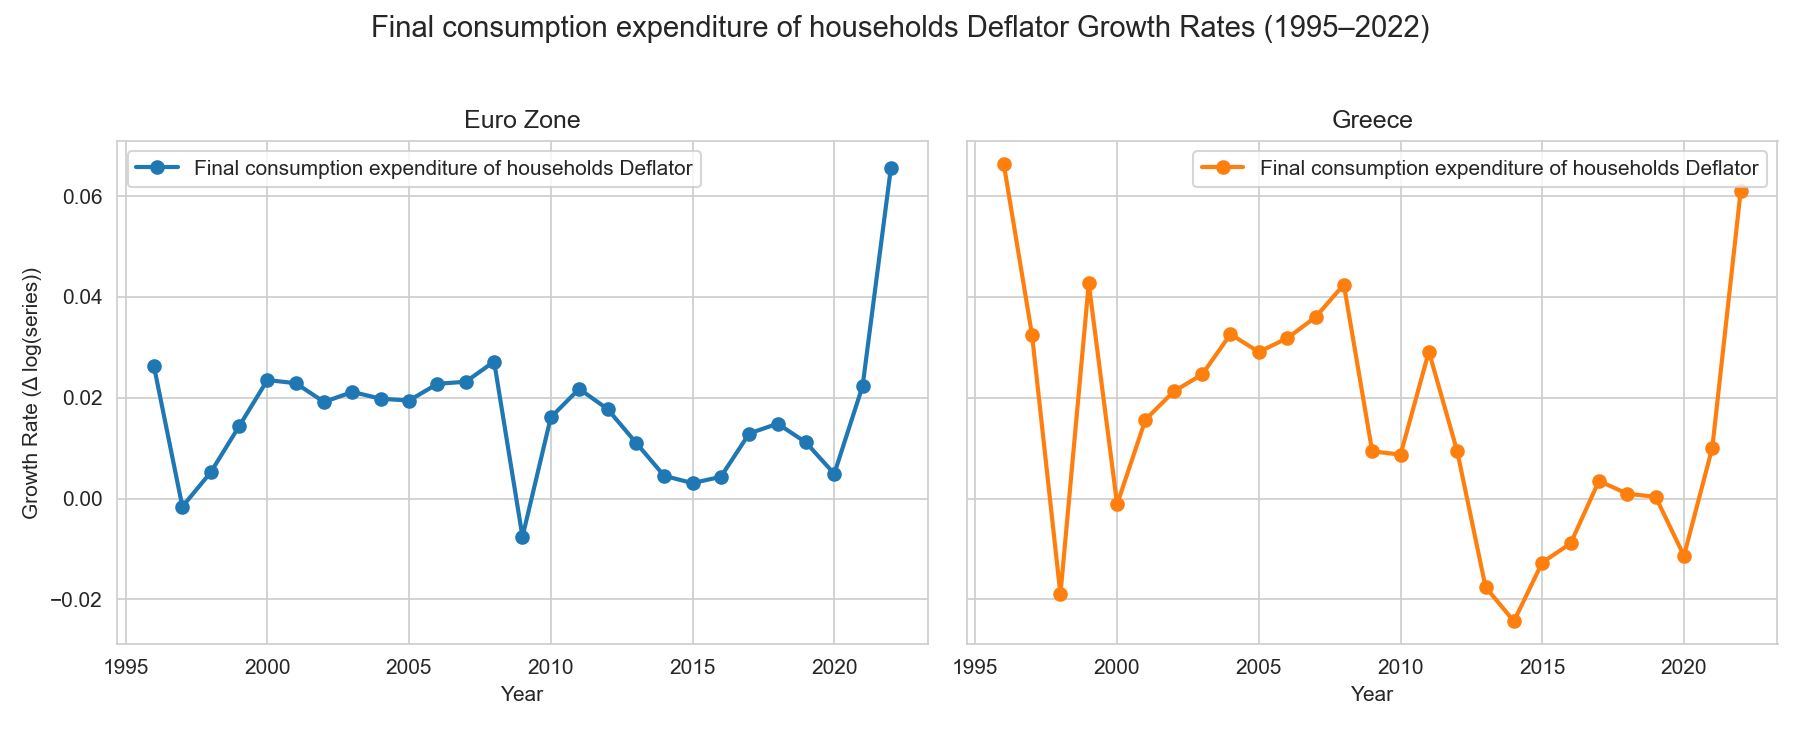
\includegraphics[width=0.8\textwidth]{Final_consumption_expenditure_of_households_deflator_growth.png}
  \vspace{0.5em}

\captionof{figure}{}\end{tcolorbox}
\FloatBarrier

\begin{tcolorbox}[colback=white,colframe=black,title={Τελικές δαπάνες κατανάλωσης νοικοκυριών: ονομαστική ανάπτυξη}]
  \centering
  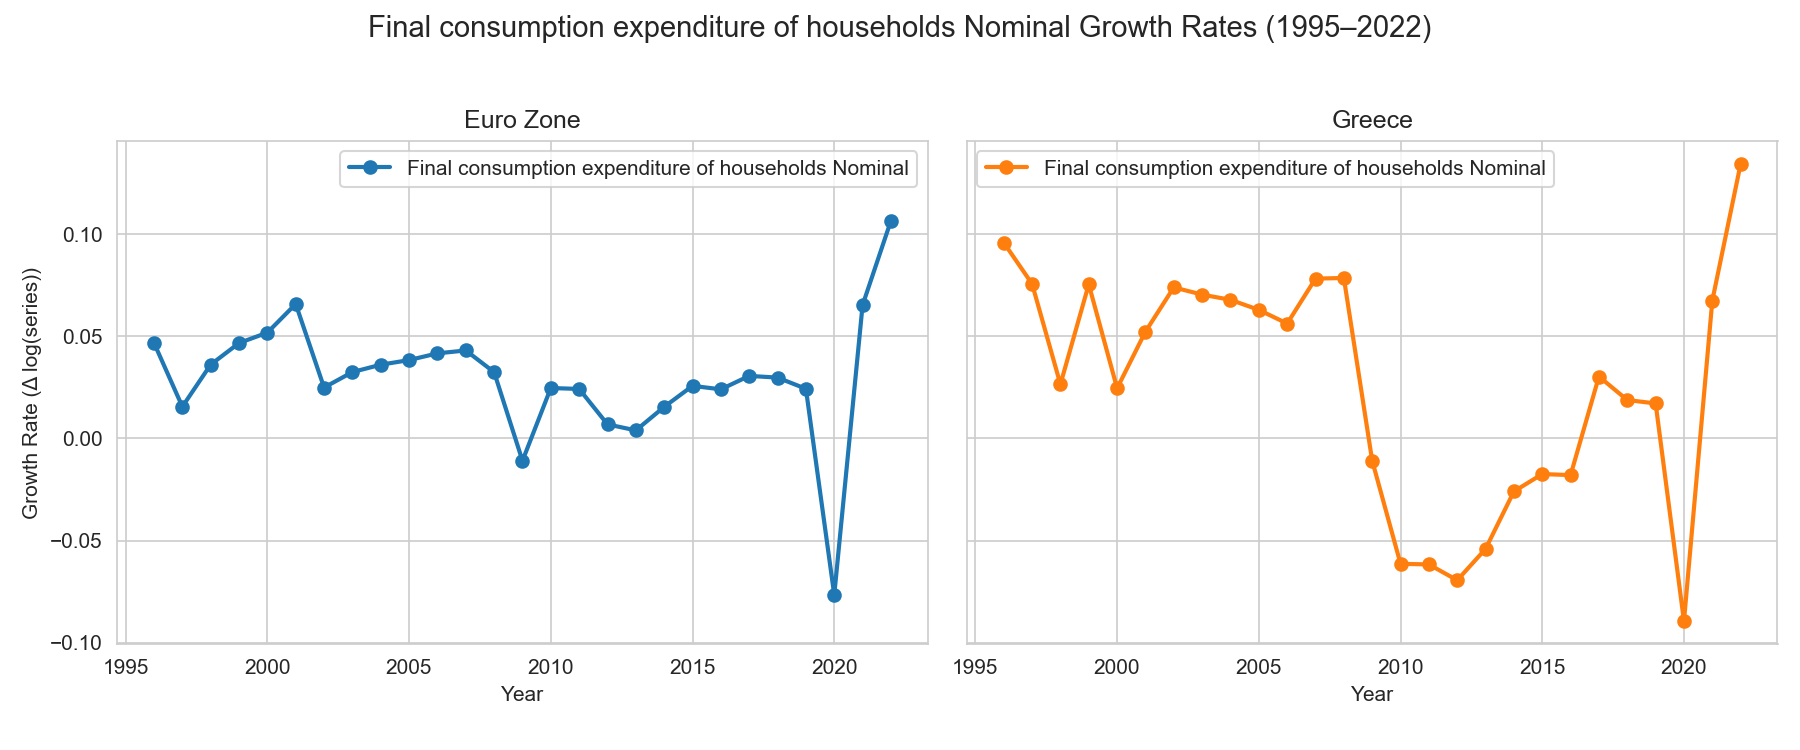
\includegraphics[width=0.8\textwidth]{Final_consumption_expenditure_of_households_nominal_growth.png}
  \vspace{0.5em}

\captionof{figure}{}\end{tcolorbox}
\FloatBarrier

% Παράδειγμα για ακαθάριστο σχηματισμό παγίου κεφαλαίου
\begin{tcolorbox}[colback=white,colframe=black,title={Ακαθάριστος σχηματισμός παγίου κεφαλαίου: ανάπτυξη αλυσίδας}]
  \centering
  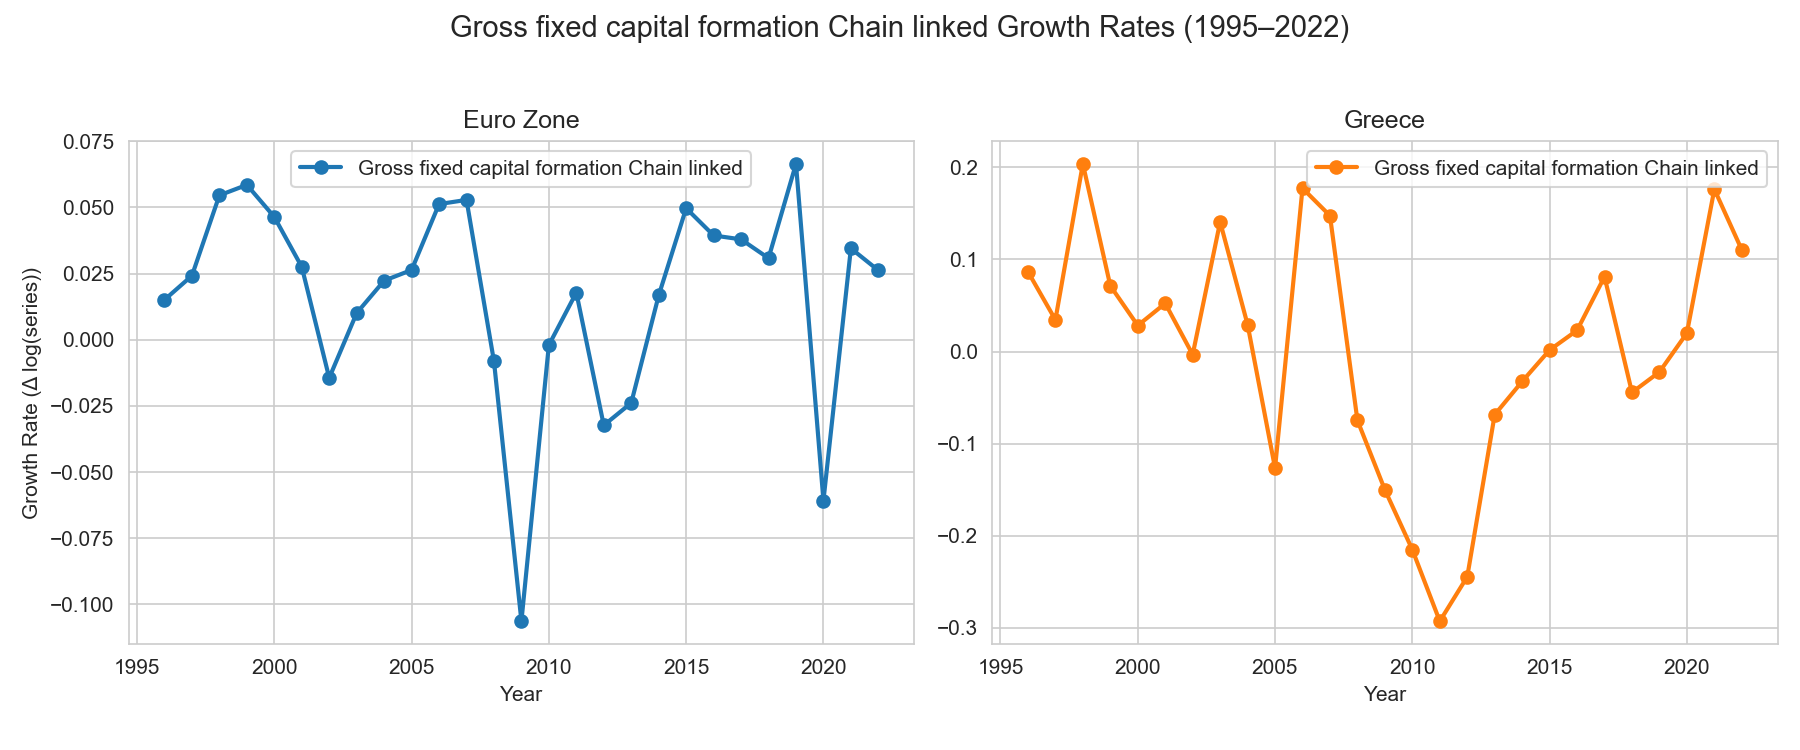
\includegraphics[width=0.8\textwidth]{Gross_fixed_capital_formation_chain_growth.png}
  \vspace{0.5em}

\captionof{figure}{}\end{tcolorbox}
\FloatBarrier

\begin{tcolorbox}[colback=white,colframe=black,title={Ακαθάριστος σχηματισμός παγίου κεφαλαίου: συνδυασμένη ανάπτυξη στην Ευρωζώνη}]
  \centering
  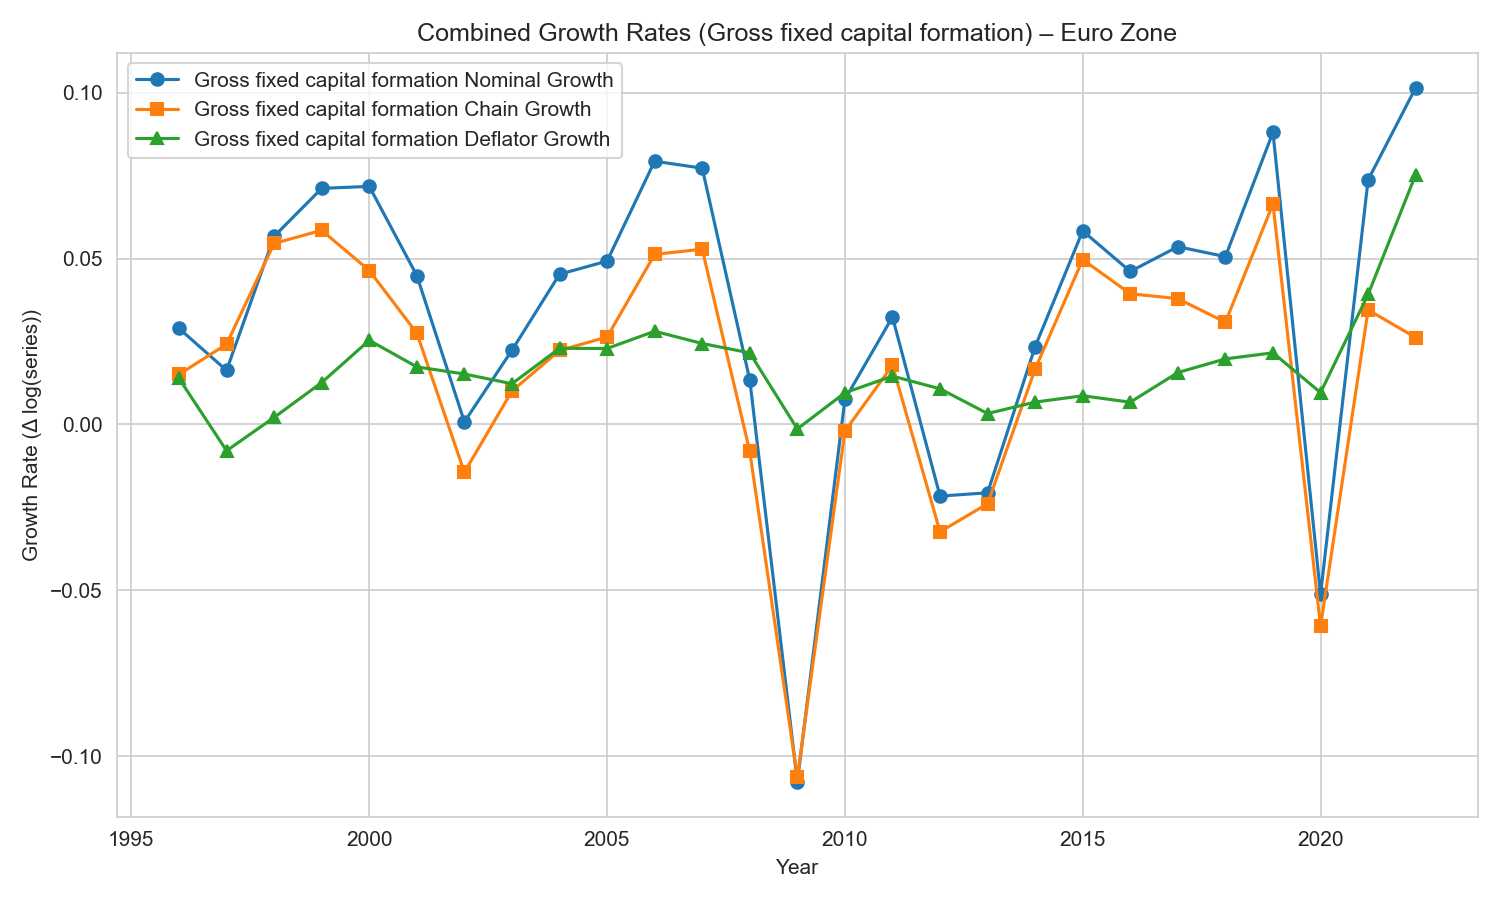
\includegraphics[width=0.8\textwidth]{Gross_fixed_capital_formation_combined_growth_Euro.png}
  \vspace{0.5em}

\captionof{figure}{}\end{tcolorbox}
\FloatBarrier

\begin{tcolorbox}[colback=white,colframe=black,title={Ακαθάριστος σχηματισμός παγίου κεφαλαίου: συνδυασμένη ανάπτυξη στην Ελλάδα}]
  \centering
  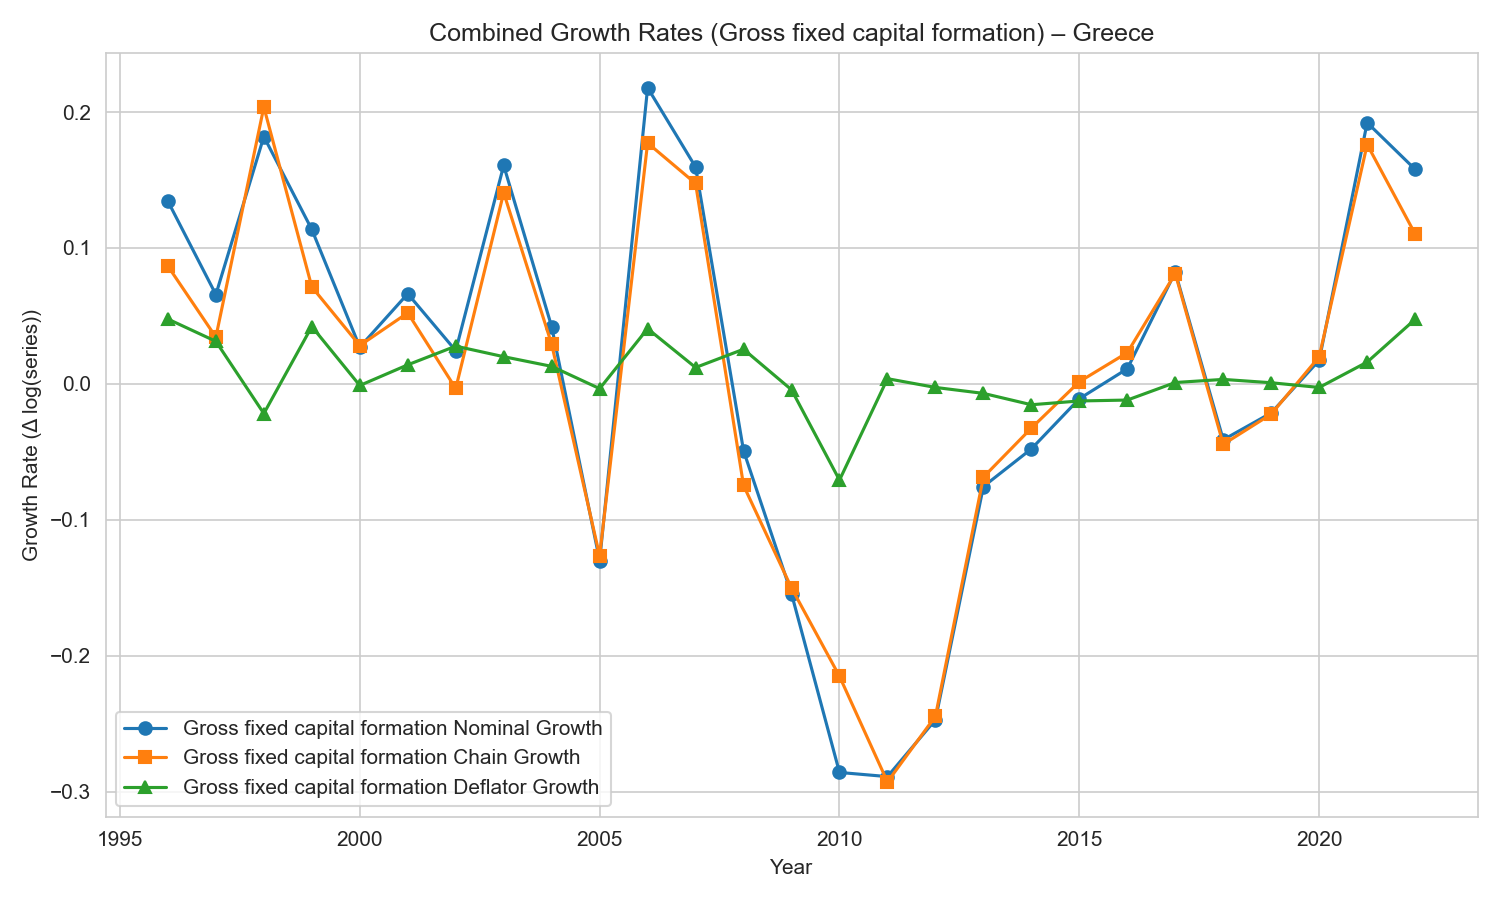
\includegraphics[width=0.8\textwidth]{Gross_fixed_capital_formation_combined_growth_Greece.png}
  \vspace{0.5em}

\captionof{figure}{}\end{tcolorbox}
\FloatBarrier

\begin{tcolorbox}[colback=white,colframe=black,title={Ακαθάριστος σχηματισμός παγίου κεφαλαίου: συνδυασμένα επίπεδα}]
  \centering
  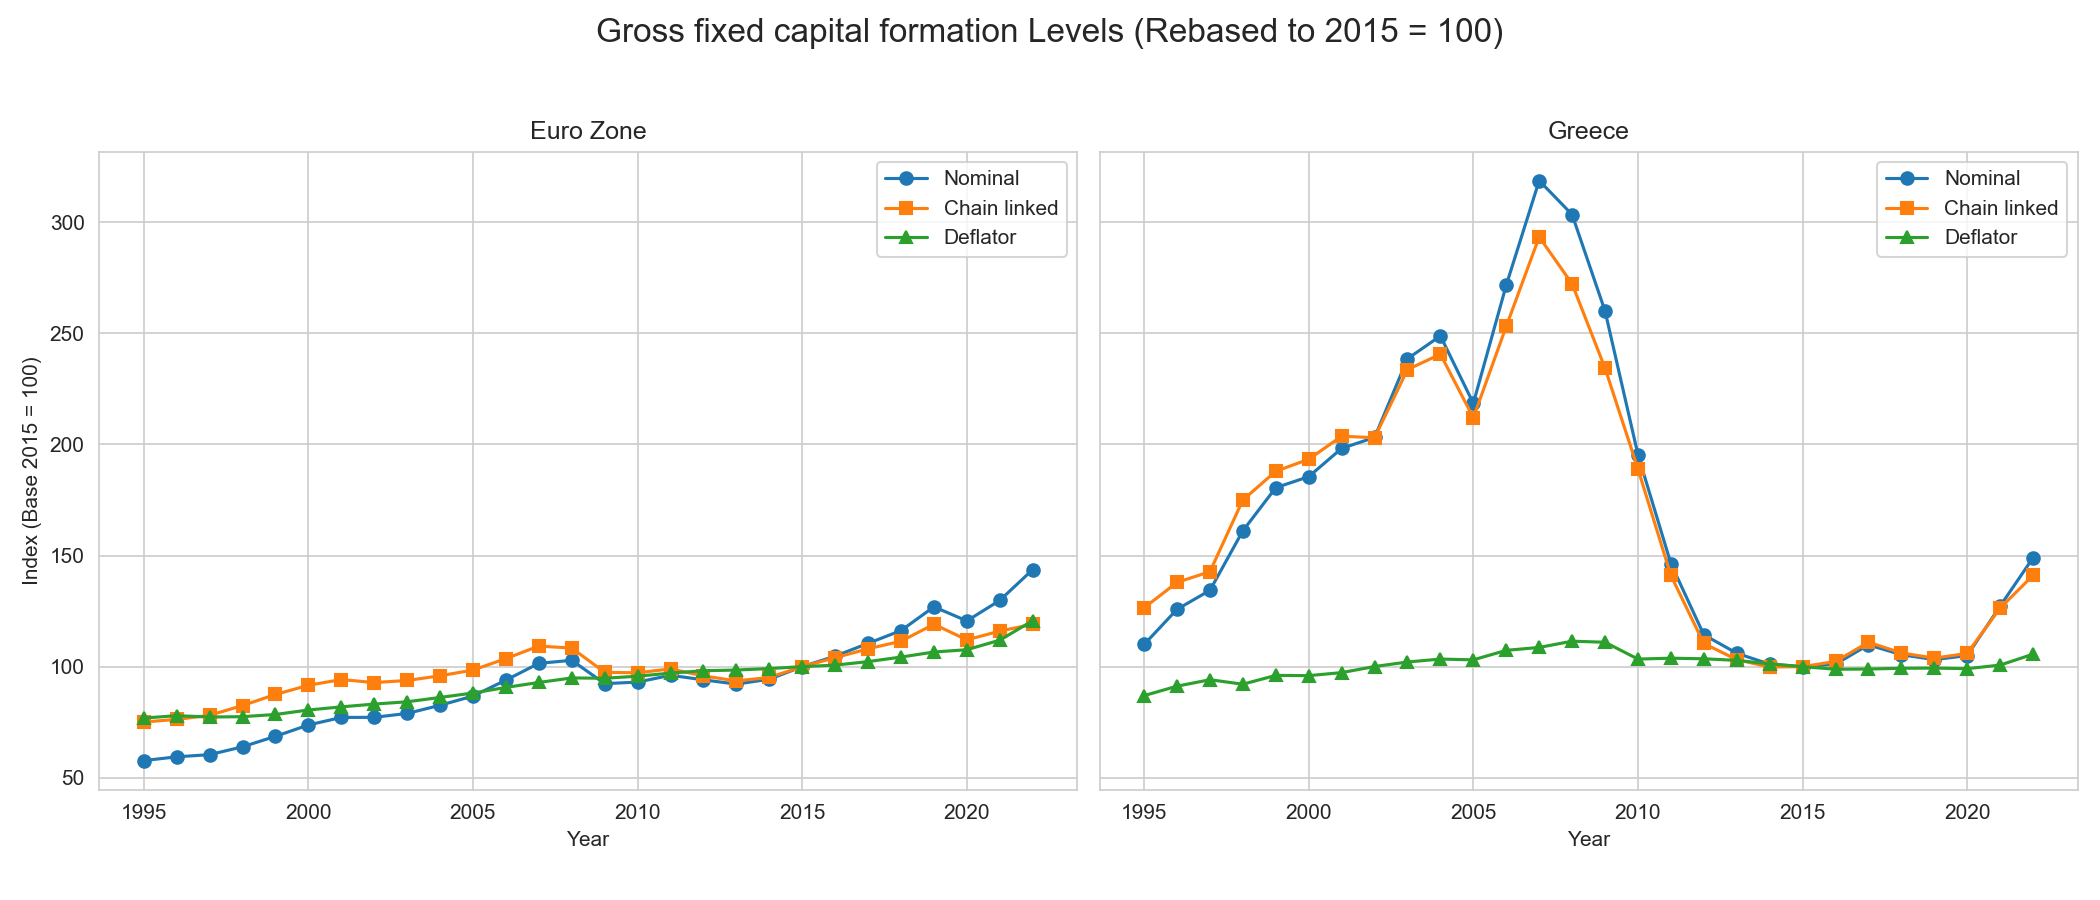
\includegraphics[width=0.8\textwidth]{Gross_fixed_capital_formation_combined_levels.png}
  \vspace{0.5em}

\captionof{figure}{}\end{tcolorbox}
\FloatBarrier

\begin{tcolorbox}[colback=white,colframe=black,title={Ακαθάριστος σχηματισμός παγίου κεφαλαίου: αποπληθωριστής}]
  \centering
  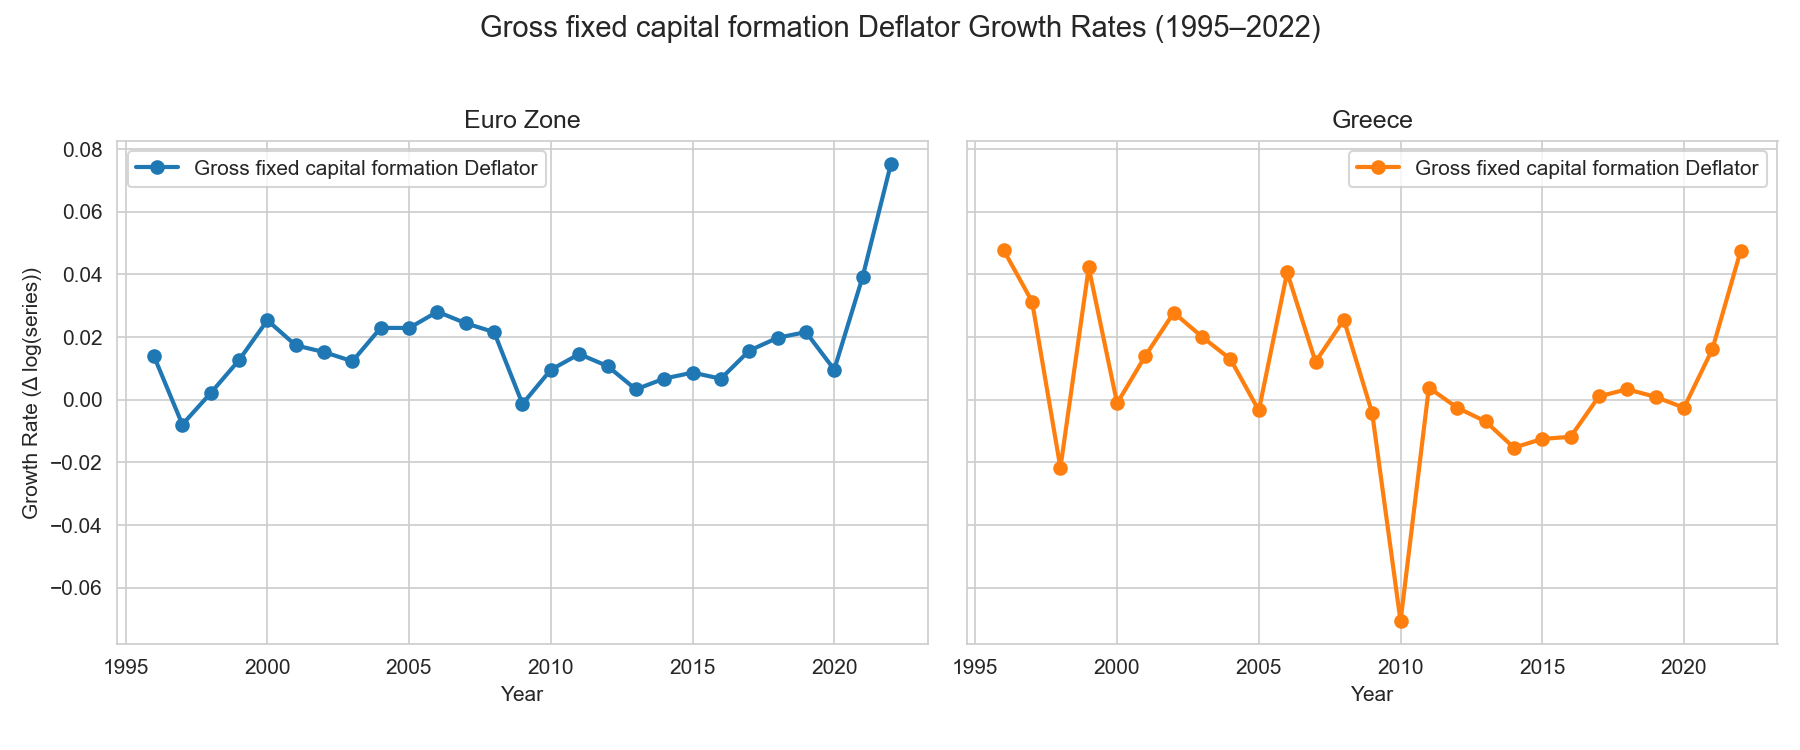
\includegraphics[width=0.8\textwidth]{Gross_fixed_capital_formation_deflator_growth.png}
  \vspace{0.5em}

\captionof{figure}{}\end{tcolorbox}
\FloatBarrier

\begin{tcolorbox}[colback=white,colframe=black,title={Ακαθάριστος σχηματισμός παγίου κεφαλαίου: ονομαστική ανάπτυξη}]
  \centering
  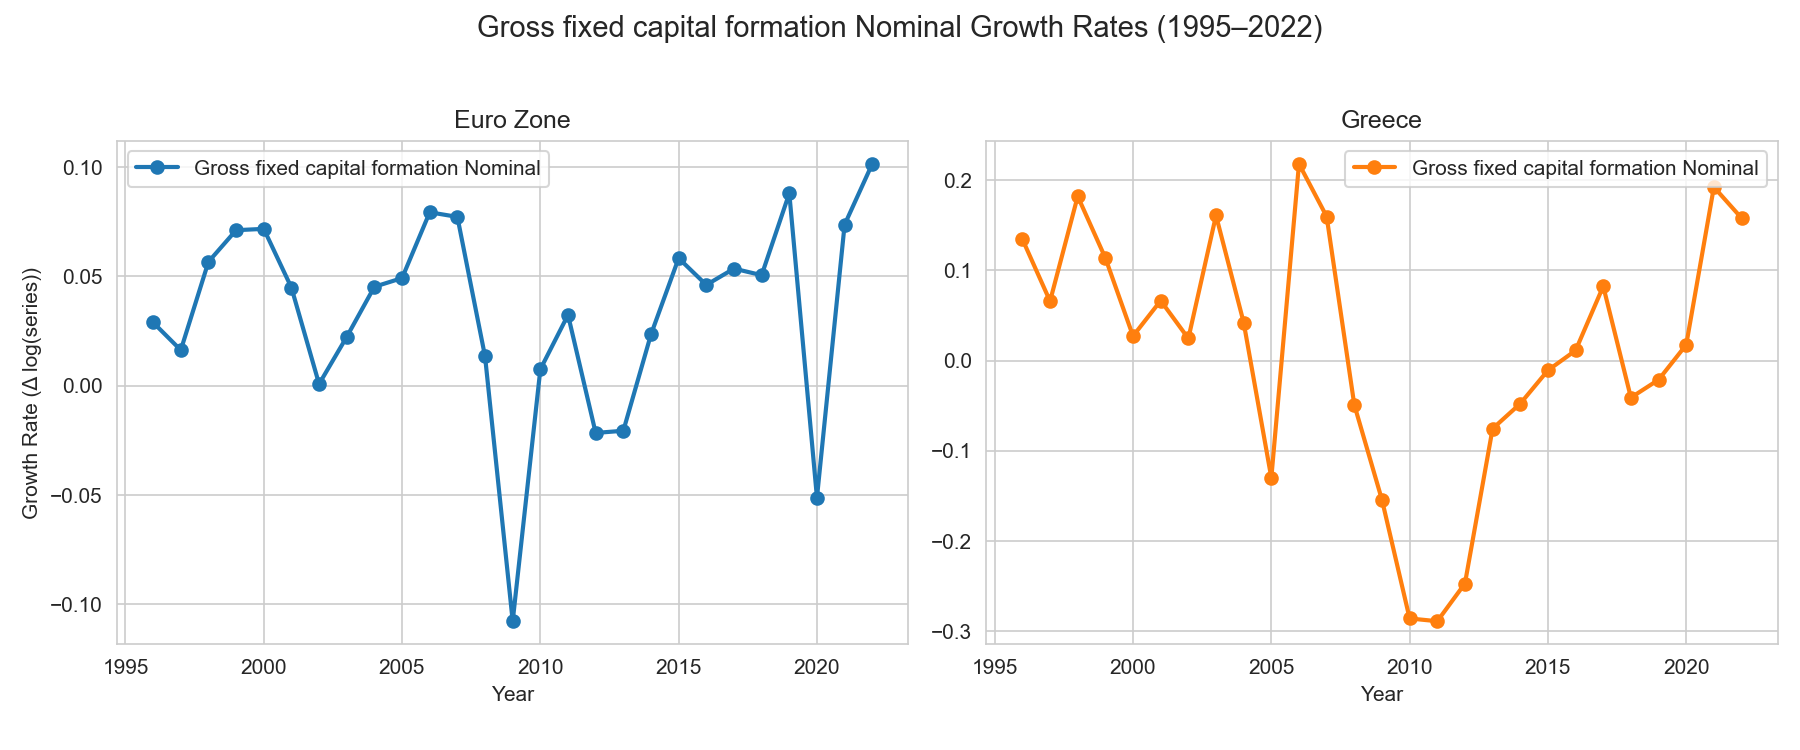
\includegraphics[width=0.8\textwidth]{Gross_fixed_capital_formation_nominal_growth.png}
  \vspace{0.5em}

\captionof{figure}{}\end{tcolorbox}
\FloatBarrier

% Παράδειγμα για Εισαγωγές αγαθών και υπηρεσιών
\begin{tcolorbox}[colback=white,colframe=black,title={Εισαγωγές αγαθών και υπηρεσιών: ανάπτυξη αλυσίδας}]
  \centering
  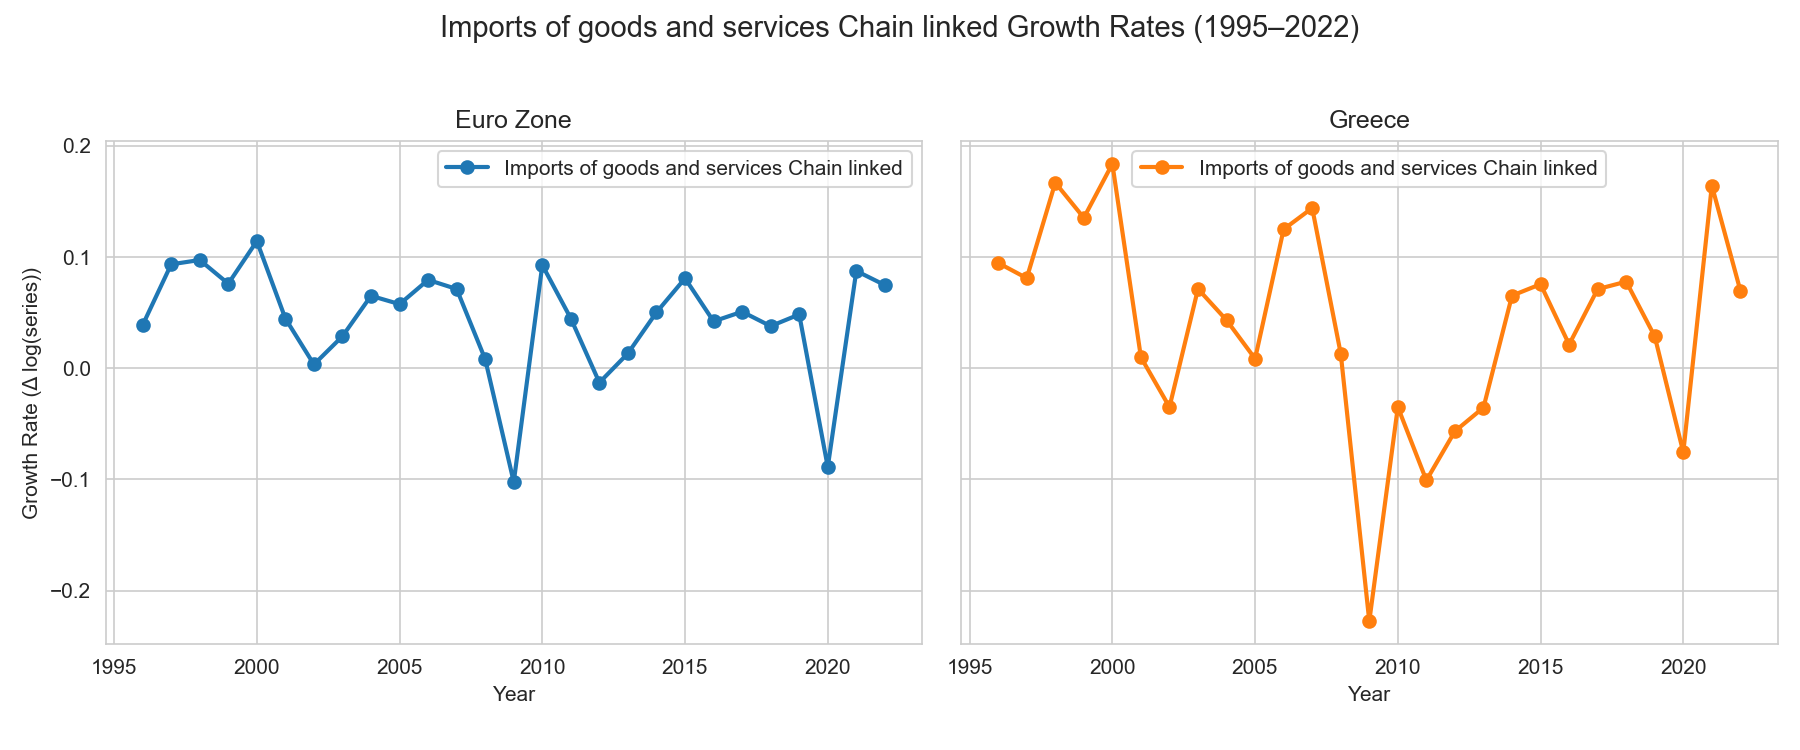
\includegraphics[width=0.8\textwidth]{Imports_of_goods_and_services_chain_growth.png}
  \vspace{0.5em}

\captionof{figure}{}\end{tcolorbox}
\FloatBarrier

\begin{tcolorbox}[colback=white,colframe=black,title={Εισαγωγές αγαθών και υπηρεσιών: συνδυασμένη ανάπτυξη στην Ευρωζώνη}]
  \centering
  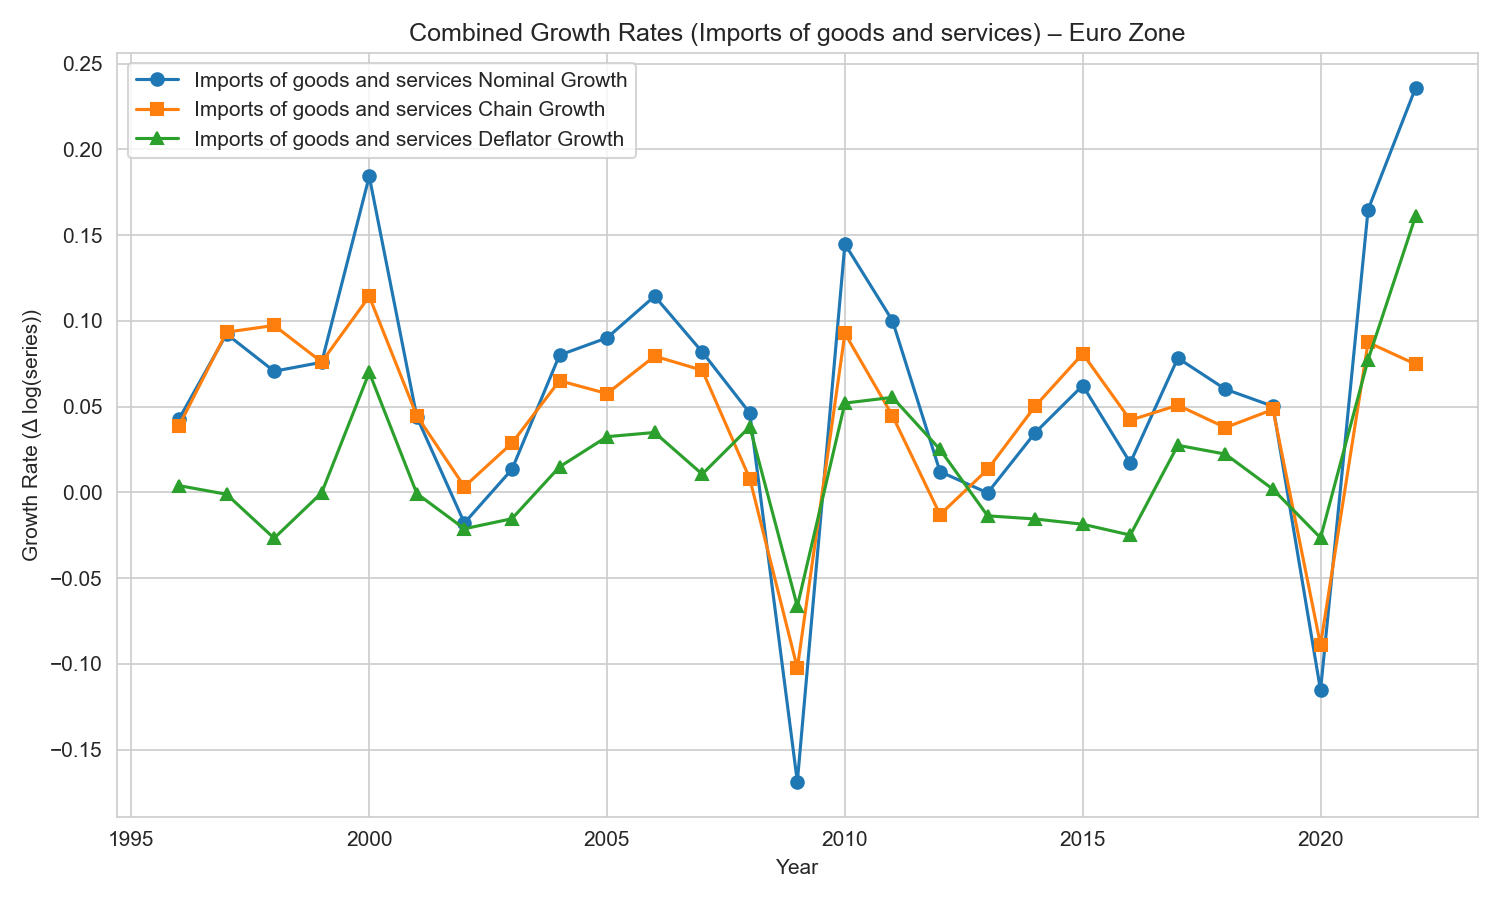
\includegraphics[width=0.8\textwidth]{Imports_of_goods_and_services_combined_growth_Euro.png}
  \vspace{0.5em}

\captionof{figure}{}\end{tcolorbox}
\FloatBarrier

\begin{tcolorbox}[colback=white,colframe=black,title={Εισαγωγές αγαθών και υπηρεσιών: συνδυασμένη ανάπτυξη στην Ελλάδα}]
  \centering
  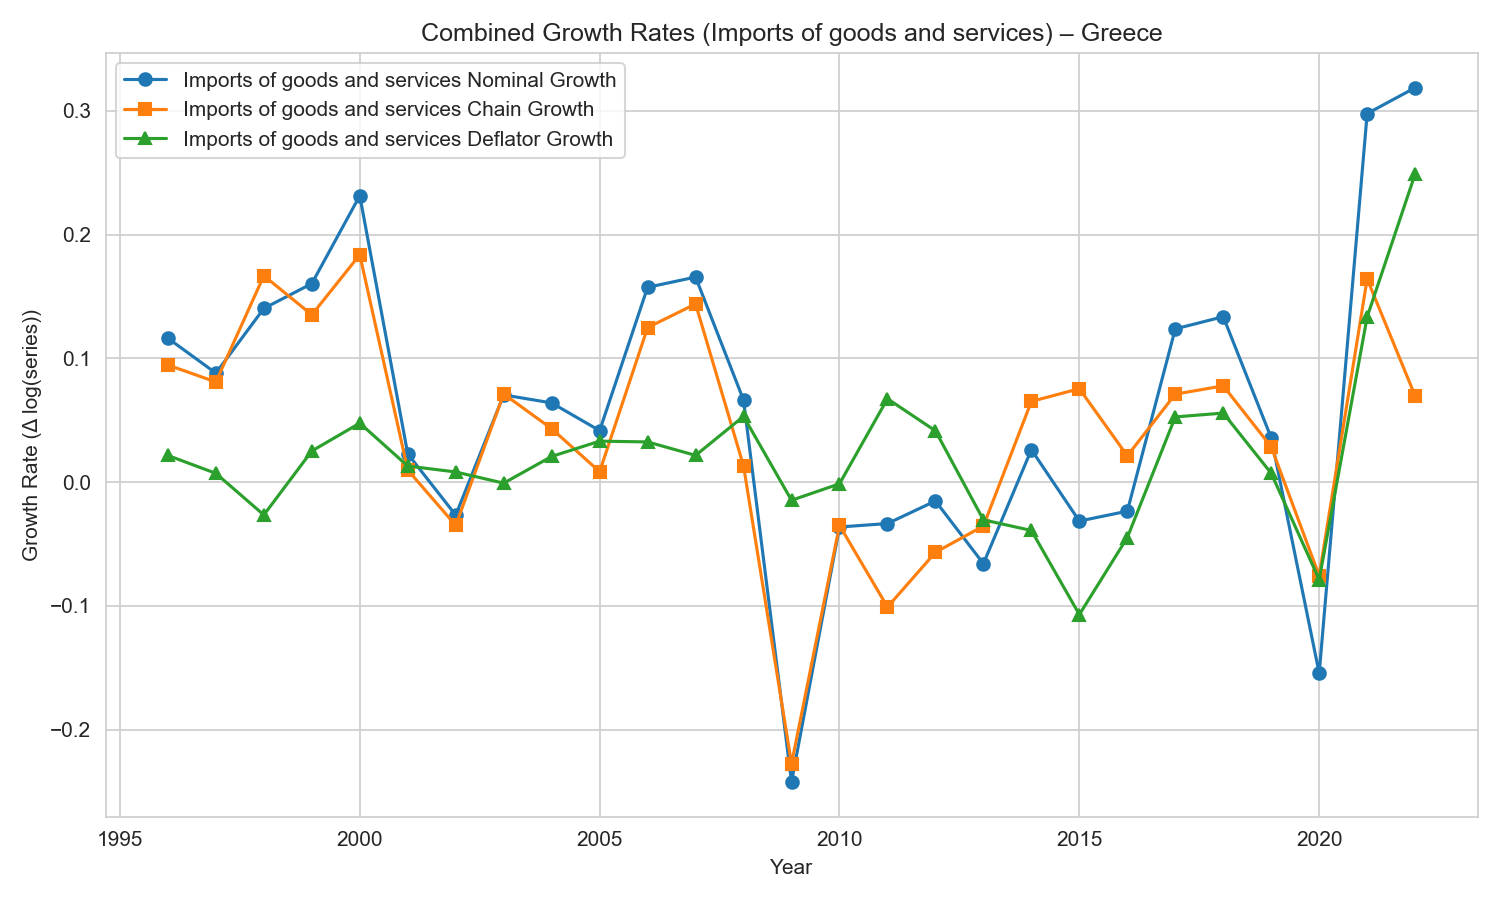
\includegraphics[width=0.8\textwidth]{Imports_of_goods_and_services_combined_growth_Greece.png}
  \vspace{0.5em}

\captionof{figure}{}\end{tcolorbox}
\FloatBarrier

\begin{tcolorbox}[colback=white,colframe=black,title={Εισαγωγές αγαθών και υπηρεσιών: συνδυασμένα επίπεδα}]
  \centering
  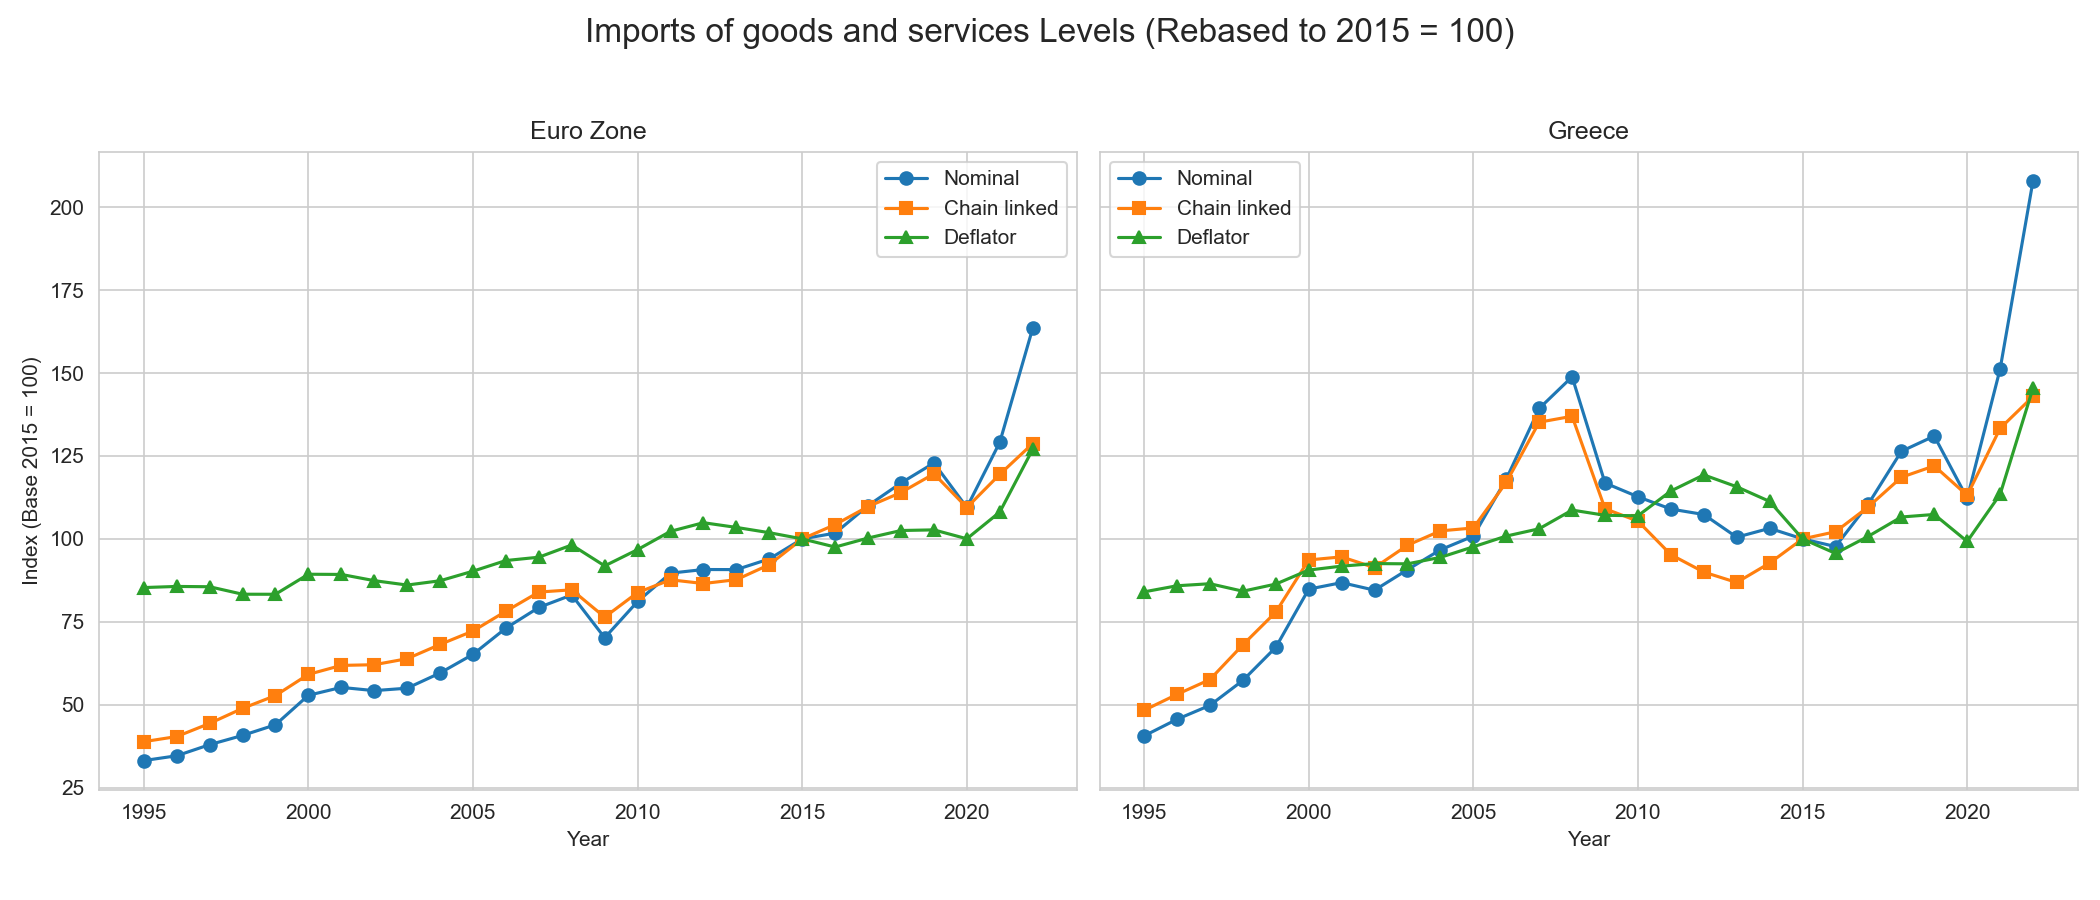
\includegraphics[width=0.8\textwidth]{Imports_of_goods_and_services_combined_levels.png}
  \vspace{0.5em}

\captionof{figure}{}\end{tcolorbox}
\FloatBarrier

\begin{tcolorbox}[colback=white,colframe=black,title={Εισαγωγές αγαθών και υπηρεσιών: αποπληθωριστής}]
  \centering
  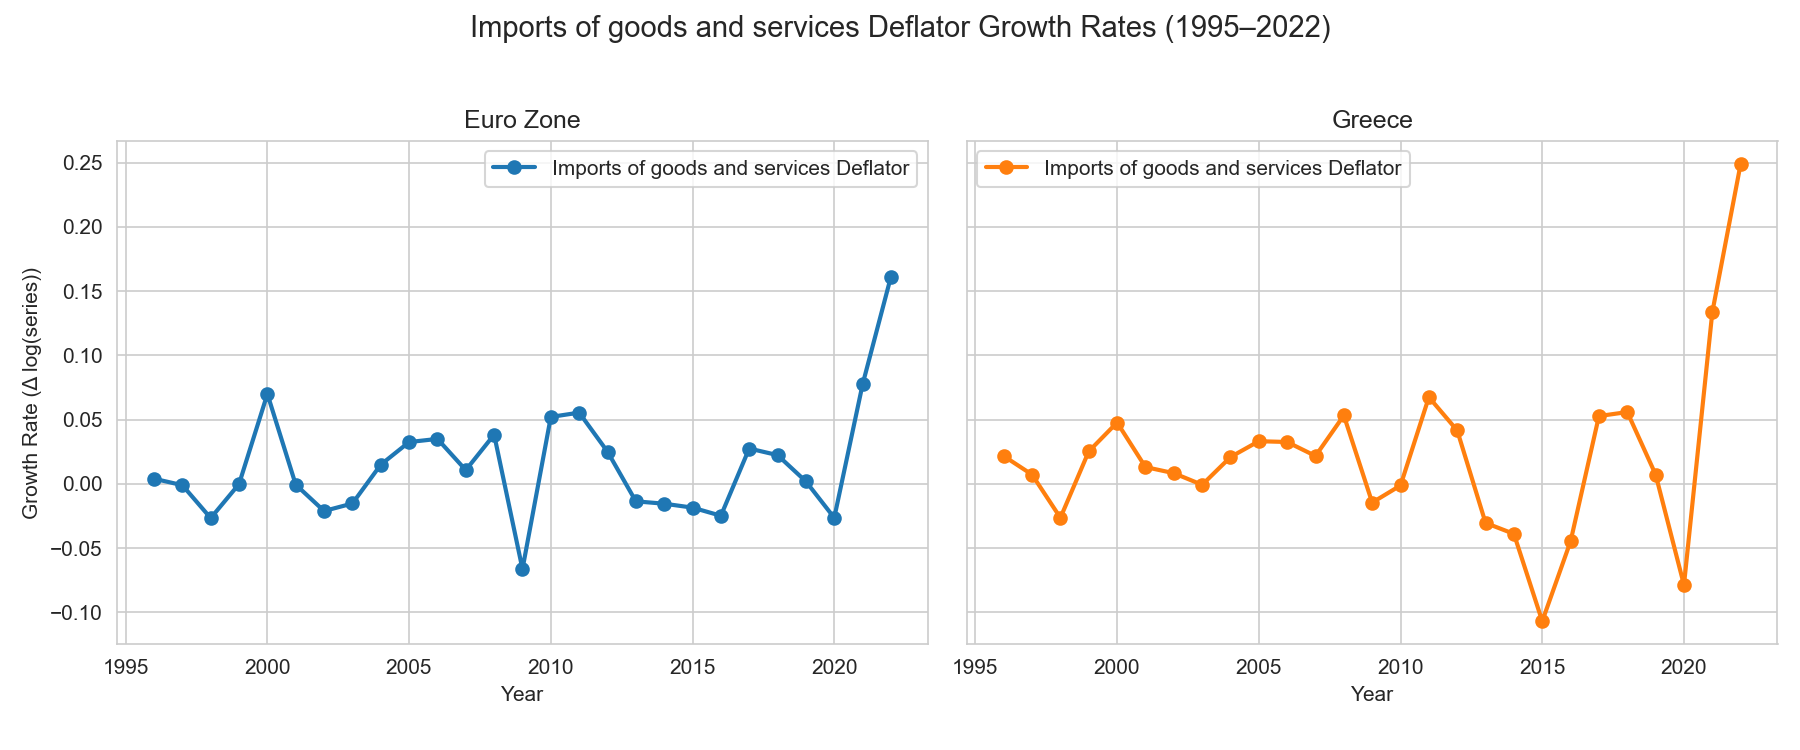
\includegraphics[width=0.8\textwidth]{Imports_of_goods_and_services_deflator_growth.png}
  \vspace{0.5em}

\captionof{figure}{}\end{tcolorbox}
\FloatBarrier

\begin{tcolorbox}[colback=white,colframe=black,title={Εισαγωγές αγαθών και υπηρεσιών: ονομαστική ανάπτυξη}]
  \centering
  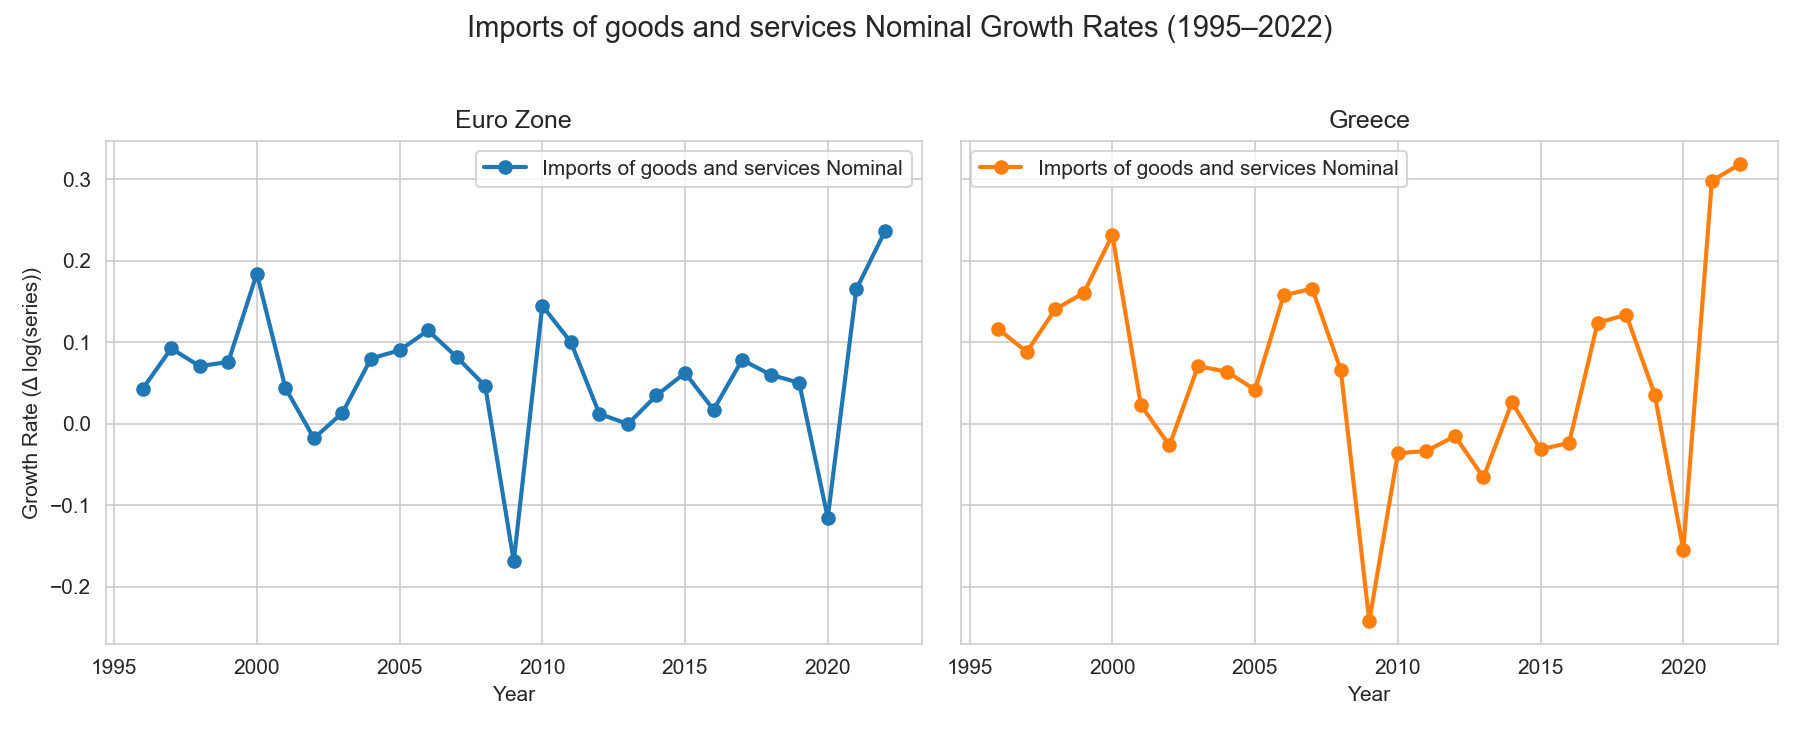
\includegraphics[width=0.8\textwidth]{Imports_of_goods_and_services_nominal_growth.png}
  \vspace{0.5em}

\captionof{figure}{}\end{tcolorbox}
\FloatBarrier

\begin{tcolorbox}[colback=white,colframe=black,title={Ονομαστικό ΑΕΠ: ανάπτυξη αλυσίδας}]
  \centering
  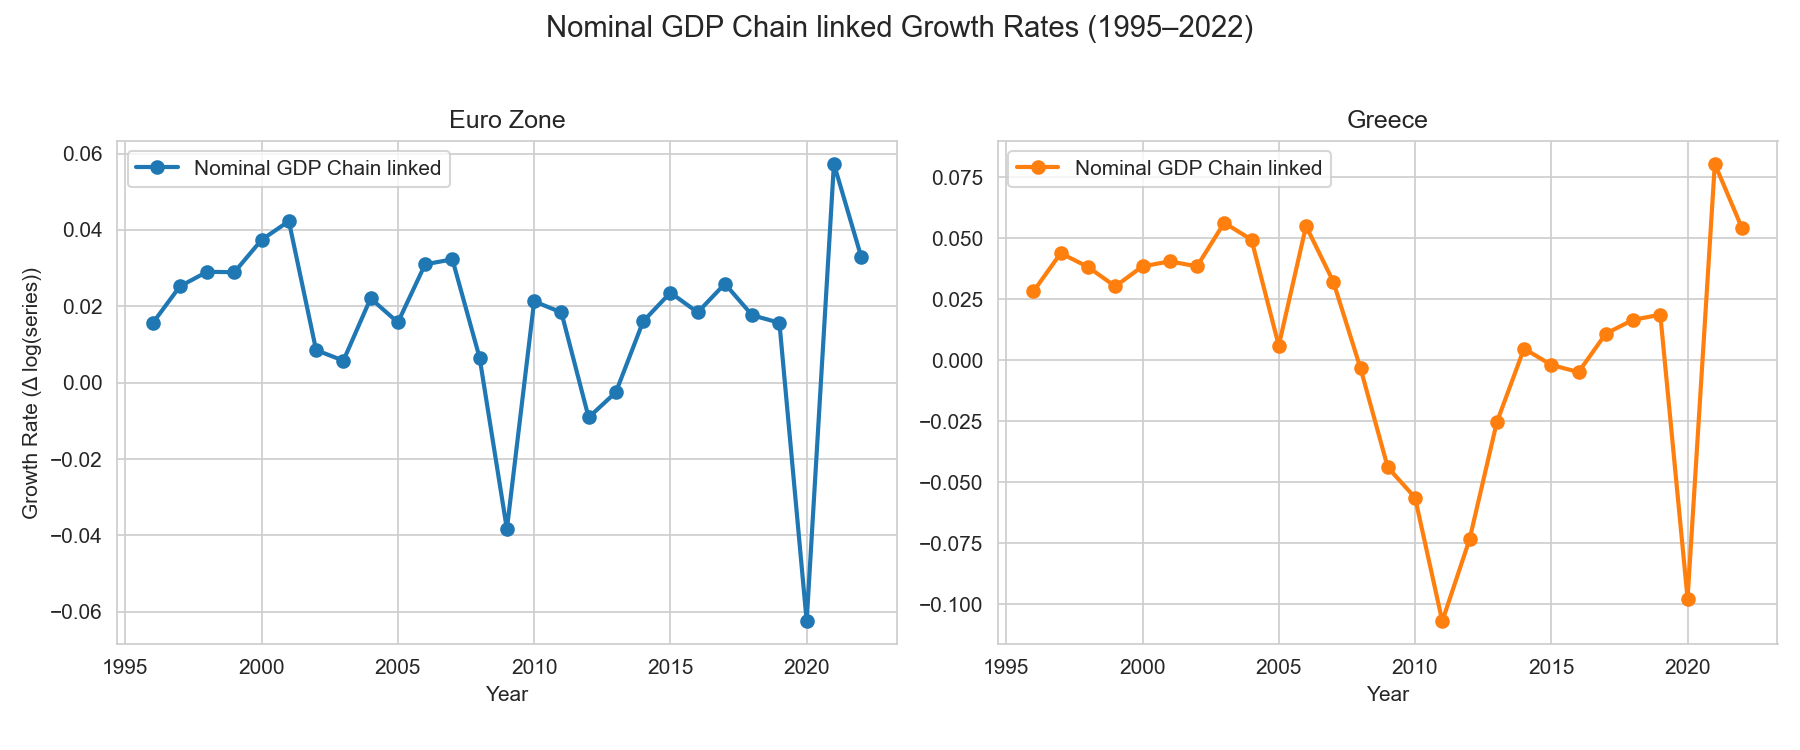
\includegraphics[width=0.8\textwidth]{Nominal_GDP_chain_growth.png}
  \vspace{0.5em}

\captionof{figure}{}\end{tcolorbox}
\FloatBarrier

\begin{tcolorbox}[colback=white,colframe=black,title={Ονομαστικό ΑΕΠ: συνδυασμένη ανάπτυξη στην Ευρωζώνη}]
  \centering
  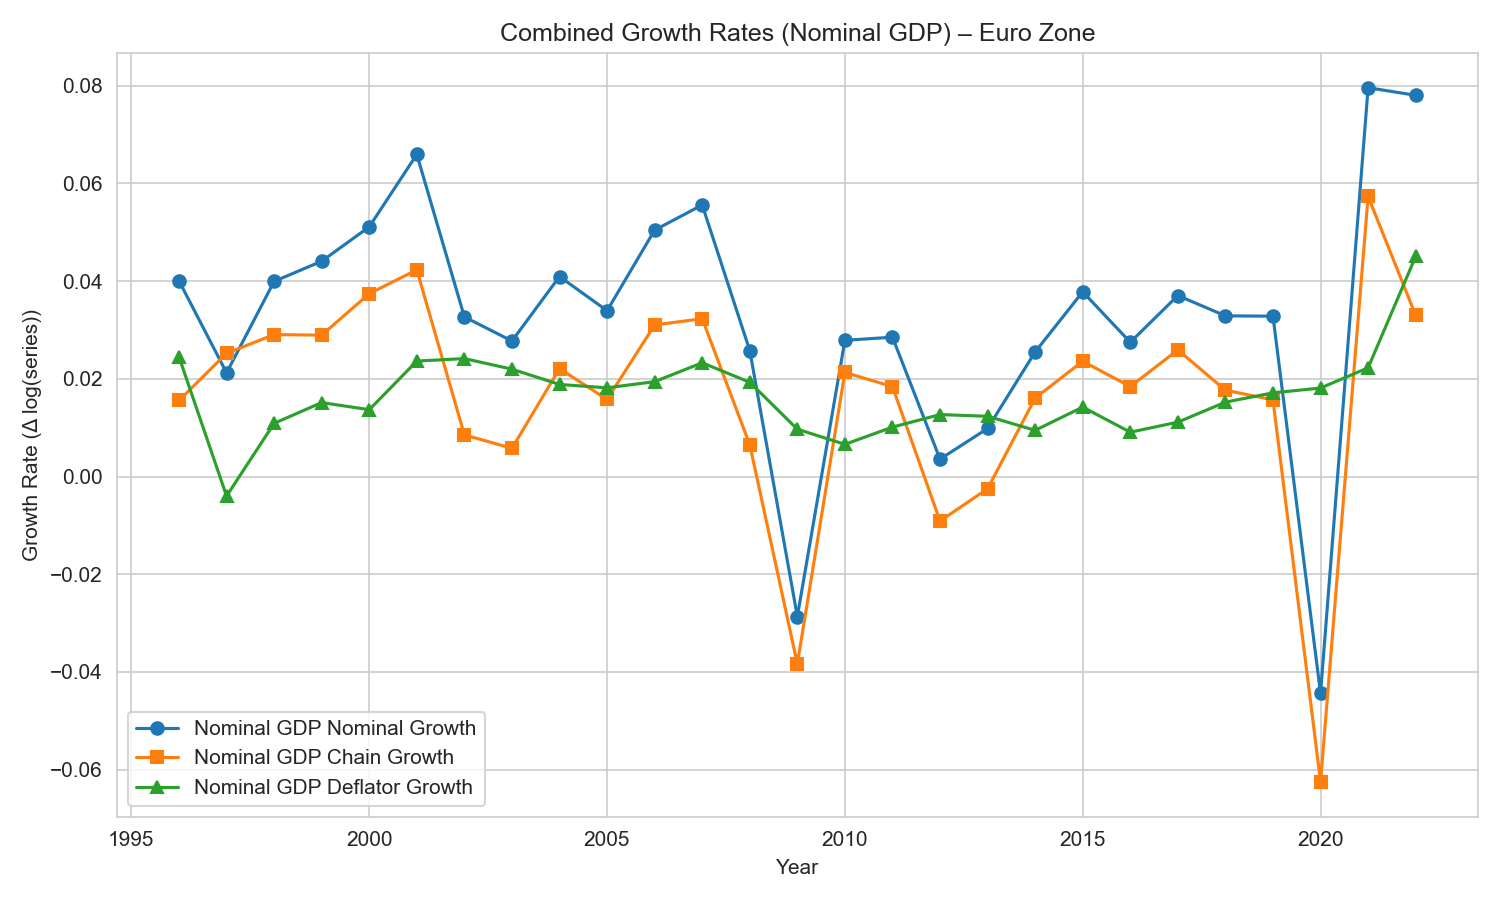
\includegraphics[width=0.8\textwidth]{Nominal_GDP_combined_growth_Euro.png}
  \vspace{0.5em}

\captionof{figure}{}\end{tcolorbox}
\FloatBarrier

\begin{tcolorbox}[colback=white,colframe=black,title={Ονομαστικό ΑΕΠ: συνδυασμένη ανάπτυξη στην Ελλάδα}]
  \centering
  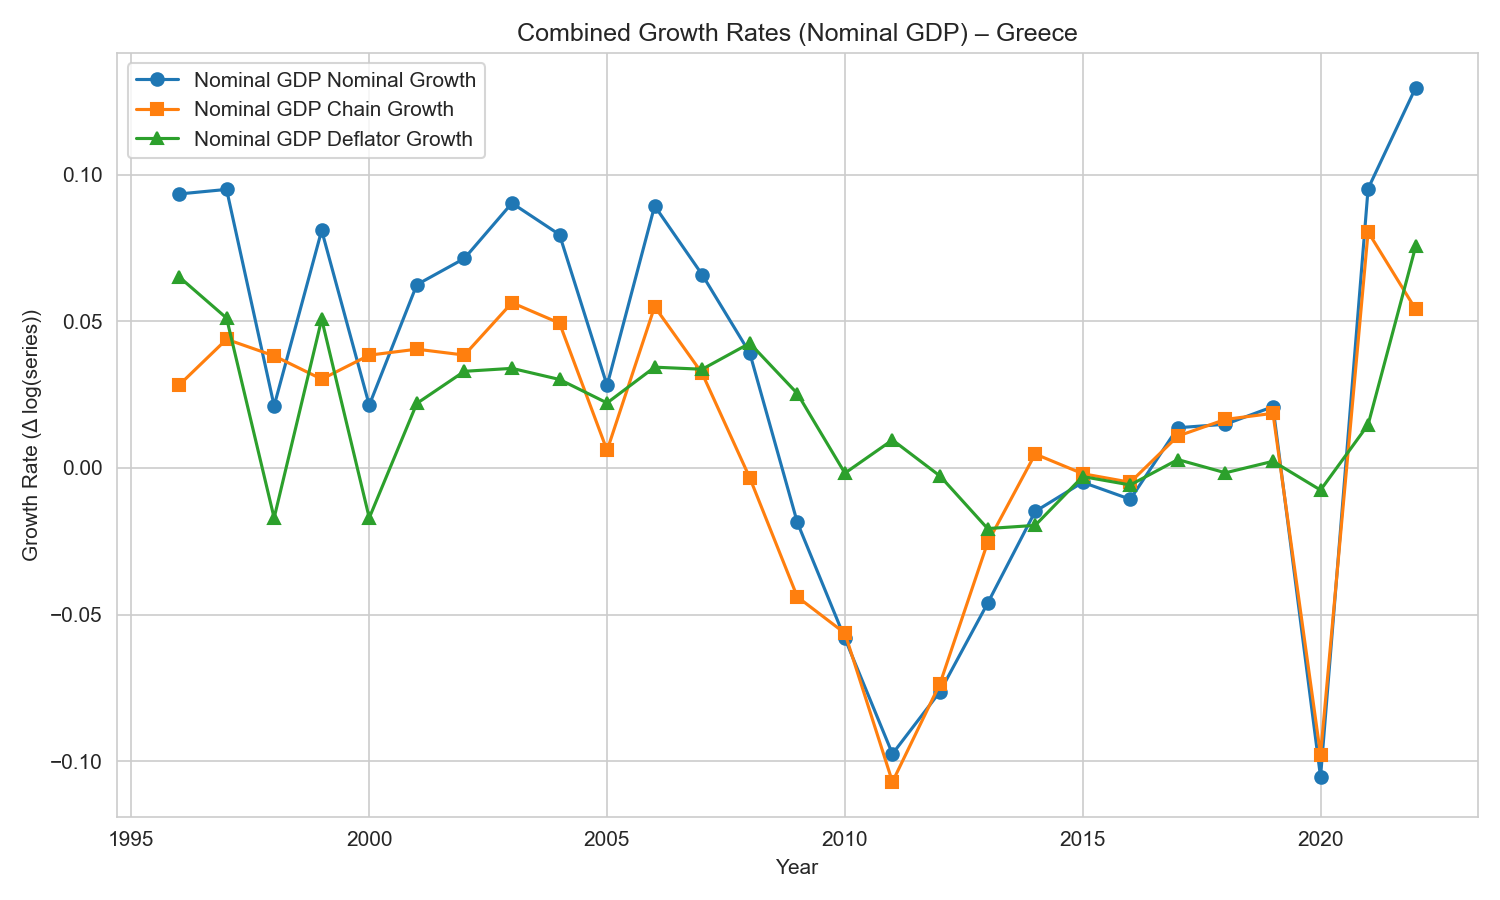
\includegraphics[width=0.8\textwidth]{Nominal_GDP_combined_growth_Greece.png}
  \vspace{0.5em}

\captionof{figure}{}\end{tcolorbox}
\FloatBarrier

\begin{tcolorbox}[colback=white,colframe=black,title={Ονομαστικό ΑΕΠ: συνδυασμένα επίπεδα}]
  \centering
  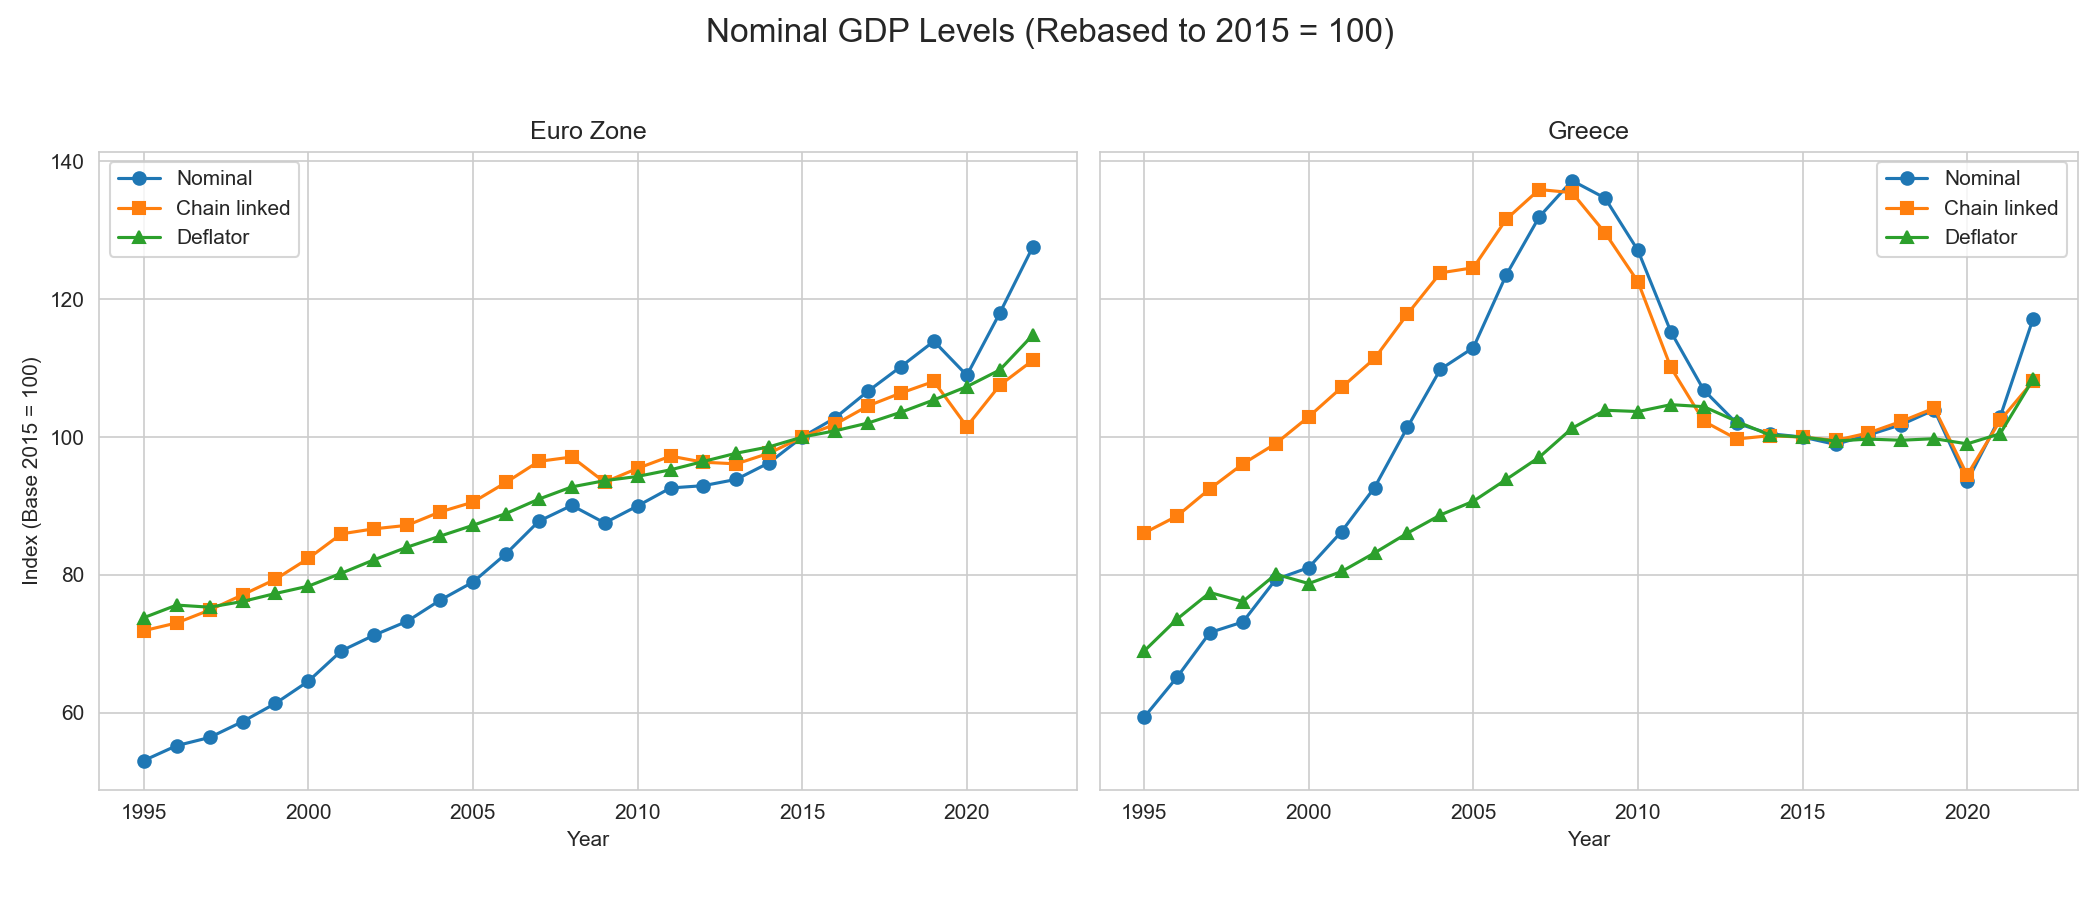
\includegraphics[width=0.8\textwidth]{Nominal_GDP_combined_levels.png}
  \vspace{0.5em}

\captionof{figure}{}\end{tcolorbox}
\FloatBarrier

\begin{tcolorbox}[colback=white,colframe=black,title={Ονομαστικό ΑΕΠ: αποπληθωριστής}]
  \centering
  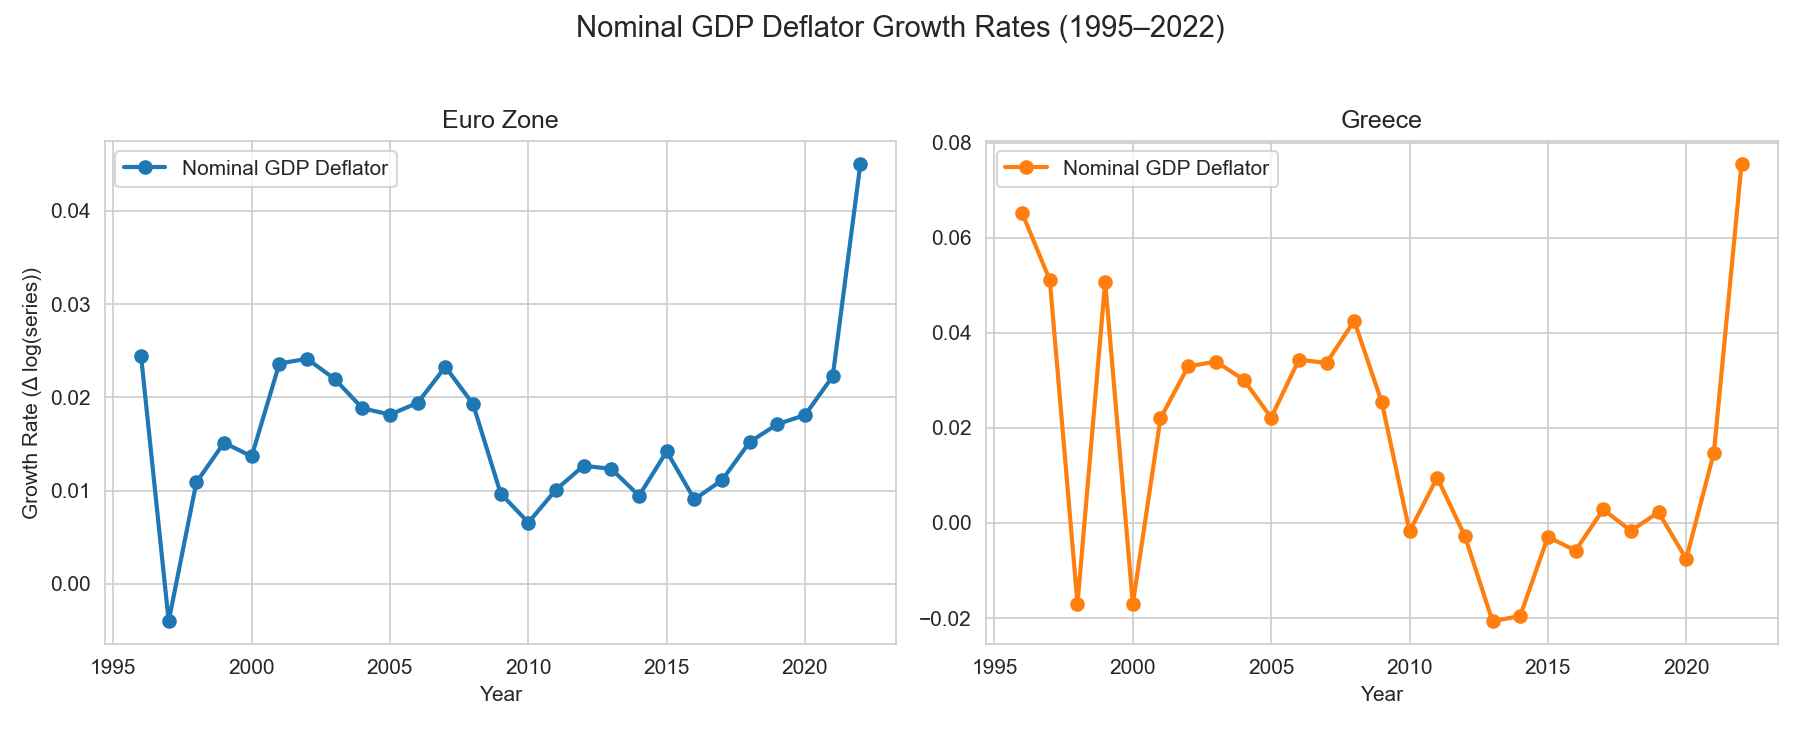
\includegraphics[width=0.8\textwidth]{Nominal_GDP_deflator_growth.png}
  \vspace{0.5em}

\captionof{figure}{}\end{tcolorbox}
\FloatBarrier

\begin{tcolorbox}[colback=white,colframe=black,title={Ονομαστικό ΑΕΠ: ονομαστική ανάπτυξη}]
  \centering
  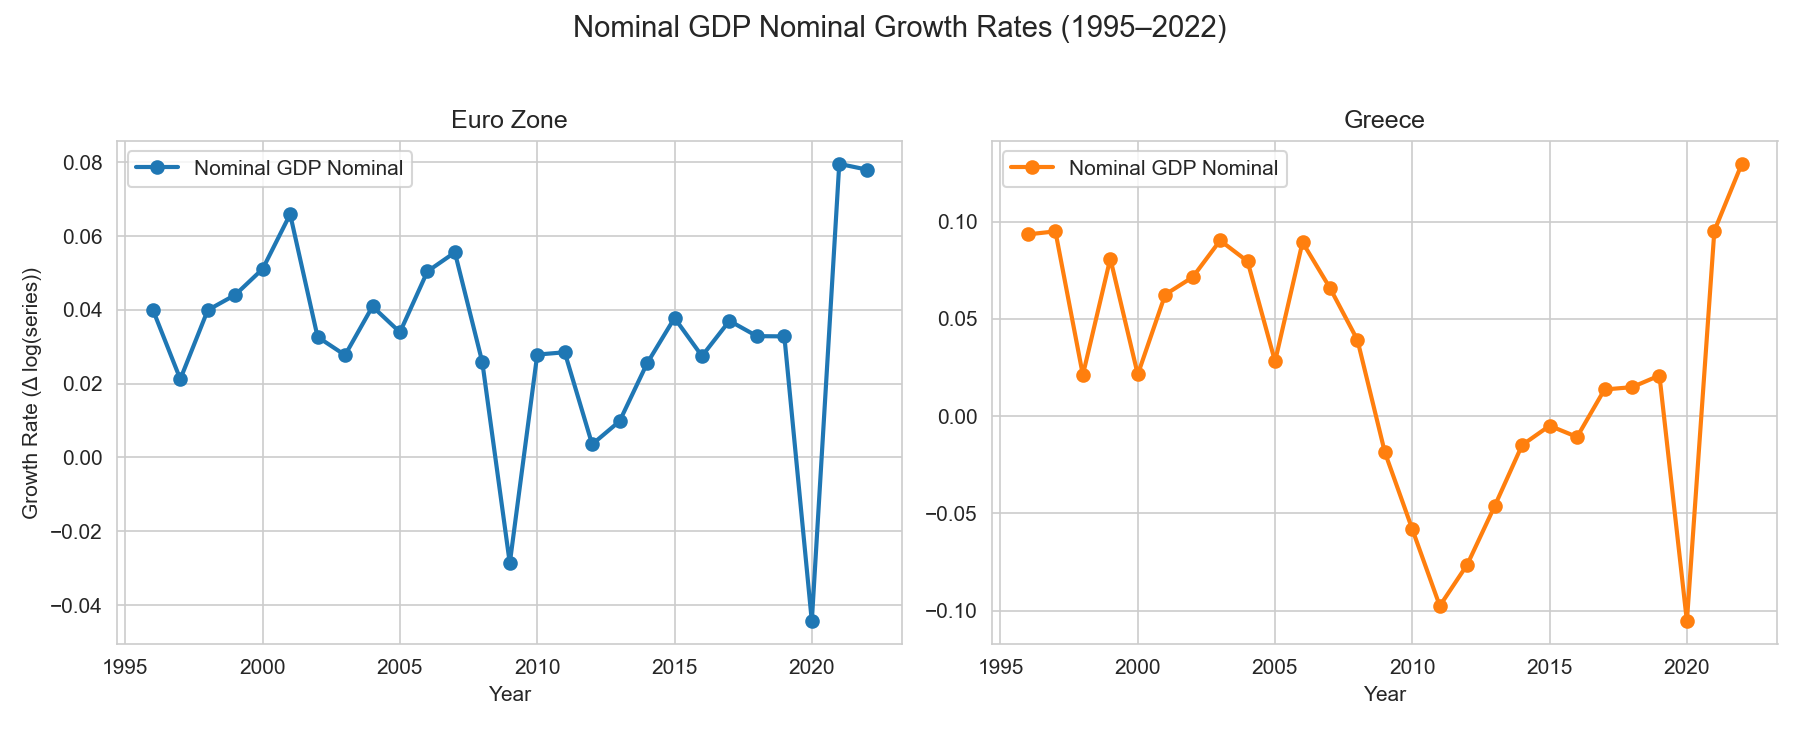
\includegraphics[width=0.8\textwidth]{Nominal_GDP_nominal_growth.png}
  \vspace{0.5em}

\captionof{figure}{}\end{tcolorbox}
\chapter{Εισαγωγή στην Άσκηση 5}
Στο πλαίσιο του \emph{MT2 Data Assignment}, η \textbf{Άσκηση 5} απαιτεί να επαναλάβουμε τα βασικά στάδια των Ασκήσεων 1--3 σε \emph{τριμηνιαία} μακροοικονομικά δεδομένα. Αυτό περιλαμβάνει:

\begin{itemize}
    \item Φόρτωση και προετοιμασία χρονολογικών σειρών από υπολογιστικό φύλλο με τριμηνιαίες παρατηρήσεις (π.χ. “Quarterly\_Data.xlsx”).
    \item Λήψη φυσικών λογαρίθμων και υπολογισμό ρυθμών μεταβολής για κάθε μεταβλητή.
    \item Δημιουργία γραφημάτων που επιτρέπουν σύγκριση μεταξύ Ευρωζώνης και Ελλάδας σε διάφορες μετρήσεις (π.χ. ΑΕΠ, τελική δαπάνη κατανάλωσης, ακαθάριστο σχηματισμό παγίου κεφαλαίου).
\end{itemize}

Παρακάτω παρουσιάζεται ένα script (\texttt{exercise\_5.py}) που υλοποιεί αυτά τα βήματα. Θα επισημάνουμε πώς κάθε τμήμα του κώδικα ανταποκρίνεται στις οδηγίες της Άσκησης 5 και εφαρμόζει ουσιαστικά τις ίδιες μεθοδολογίες από τις Ασκήσεις 1--3 σε \emph{τριμηνιαία} δεδομένα.

\section{Φόρτωση \& Καθαρισμός Τριμηνιαίων Δεδομένων}
Αρχικά, ο κώδικας συσχετίζει ονόματα μεταβλητών (π.χ. «Gross domestic product at market prices», «Final consumption expenditure») με συγκεκριμένα φύλλα στο \texttt{Quarterly\_Data.xlsx}. Ύστερα ορίζεται μια συνάρτηση \texttt{clean\_cell} για να επεξεργάζεται κάθε κελί, αφαιρώντας ανεπιθύμητους χαρακτήρες (π.χ. \texttt{p, b} στο τέλος) και μετατρέποντας αριθμητικές συμβολοσειρές σε \texttt{float}.

\begin{tcolorbox}[colback=white,colframe=black,title=Απόσπασμα Κώδικα: Φύλλα Καθαρισμός Κελιών]
\begin{lstlisting}[language=Python]
  sheet_info = {
    "Gross domestic product at market prices": {
        "Nominal": "Sheet 40",  # Current prices, million euro
        "Deflator": "Sheet 79"  # Price index (implicit deflator), 2015=100, euro
    },
    "Final consumption expenditure": {
        "Nominal": "Sheet 42",  # Current prices, million euro
        "Deflator": "Sheet 81"  # Price index (implicit deflator), 2015=100, euro
    },
    "Gross fixed capital formation": {
        "Nominal": "Sheet 51",  # Current prices, million euro
        "Deflator": "Sheet 90"  # Price index (implicit deflator), 2015=100, euro
    }
}


excel_file = "Quarterly_Data.xlsx"

def clean_cell(cell):
    """
    Καθαρίζει την τιμή ενός κελιού:
      - Εάν το κελί ισούται με ":", επιστρέφει np.nan.
      - Εάν περιέχει αριθμό με επιπλέον σύμβολα (π.χ. "123p"), αφαιρεί
        μη αριθμητικούς χαρακτήρες και παίρνει μόνο το αριθμητικό τμήμα.
      - Αλλιώς προσπαθεί να το μετατρέψει σε float.
    """
    ...
\end{lstlisting}
\end{tcolorbox}

\subsection*{Πώς κόβονται τα δεδομένα}
\begin{itemize}
  \item Ο κώδικας εντοπίζει τη γραμμή όπου εμφανίζονται οι ετικέτες τριμήνων (π.χ. \texttt{"1995-Q1", "1995-Q2", ...}) και τη στήλη από την οποία ξεκινούν τα δεδομένα του \texttt{1995-Q1}.
  \item Έπειτα διαβάζει τις σειρές της Ευρωζώνης (π.χ. γραμμή 12) και της Ελλάδας (π.χ. γραμμή 13) από το φύλλο \texttt{Quarterly\_Data.xlsx}, αποθηκεύοντάς τες σε ένα \texttt{DataFrame} δύο στηλών (Euro Area, Greece).
  \item Τα κενά δεδομένα γεμίζονται με \texttt{ffill} (προηγούμενη τιμή) ή \texttt{bfill} (επόμενη τιμή), ώστε να μην υπάρχουν κενά στα τελικά αποτελέσματα.
\end{itemize}

\section{Υπολογισμός Ρυθμών Μεταβολής}
Σύμφωνα με τις Ασκήσεις 1--3, ο κώδικας λαμβάνει τους φυσικούς λογαρίθμους και στη συνέχεια υπολογίζει τις πρώτες διαφορές (\(\Delta \log(\text{series})\)) για τον ρυθμό μεταβολής.

\begin{tcolorbox}[colback=white,colframe=black,title=Απόσπασμα Κώδικα: Ρυθμοί Μεταβολής]
\begin{lstlisting}[language=Python]
def compute_growth(df):
    """
    Υπολογίζει ρυθμούς μεταβολής ως πρώτη διαφορά του φυσικού λογαρίθμου.
    Αναμένεται ότι το DataFrame περιέχει αριθμητικά δεδομένα χωρίς NaNs.
    """
    df = df.replace(0, np.nan).ffill().bfill()
    log_vals = np.log(df)
    growth = log_vals.diff().iloc[1:]
    return growth
\end{lstlisting}
\end{tcolorbox}

\subsection*{Επεξήγηση}
\begin{itemize}
  \item Μέσω \(\Delta \log(\cdot)\) εξάγονται οι ποσοστιαίες μεταβολές από τρίμηνο σε τρίμηνο.
  \item Τυχόν μηδενικές τιμές αντικαθίστανται με \texttt{NaN} πριν τον λογαριθμισμό, ώστε να αποφευχθούν σφάλματα.
\end{itemize}

\section{Διαγράμματα Τριμηνιαίων Ρυθμών Μεταβολής}
Στη συνέχεια δημιουργούνται διαγράμματα σε μορφή στοίβας (stacked), με την Ευρωζώνη από πάνω και την Ελλάδα από κάτω, ώστε να φαίνεται ευδιάκριτα η σύγκριση των ρυθμών μεταβολής μεταξύ των δύο περιοχών.

\begin{tcolorbox}[colback=white,colframe=black,title=Απόσπασμα Κώδικα: Σχεδιασμός Τριμηνιαίων Ρυθμών Μεταβολής]
\begin{lstlisting}[language=Python]
def plot_growth_stacked(x, x_labels, growth_df, var_name, filename):
    """
    Δημιουργεί γράφημα με 2 υπο-διαγράμματα (Euro Zone, Greece) για Δ log(series).
    Εμφανίζει μόνο κάθε 20ή ετικέτα τριμήνου για μεγαλύτερη ευκρίνεια.
    """
    ...
    fig, axs = plt.subplots(2, 1, figsize=(16,12), dpi=150, sharex=True)
    axs[0].plot(x, growth_values[:,0], marker='o', linestyle='-', linewidth=2, color='tab:blue')
    axs[0].set_title("Euro Zone")
    ...
    axs[1].plot(x, growth_values[:,1], marker='o', linestyle='-', linewidth=2, color='tab:orange')
    axs[1].set_title("Greece")
    ...
    plt.savefig(filename)
\end{lstlisting}
\end{tcolorbox}

\subsection*{Επεξήγηση}
\begin{itemize}
  \item Ο πίνακας \texttt{x\_labels} περιέχει τις ετικέτες (π.χ. «1995-Q1»), ωστόσο στο διάγραμμα εμφανίζονται αραιωμένες (π.χ. κάθε 20ο τρίμηνο) για να μη γεμίσει υπερβολικά ο \textit{x}-άξονας.
  \item Στο τέλος, το γράφημα αποθηκεύεται σε μορφή \texttt{.png}.
\end{itemize}


\chapter{Παράρτημα: Επιπλέον Γραφήματα (Άσκηση 5)}

% Ορίζουμε το path, αν θέλουμε να μην το γράφουμε συνέχεια.
% Εναλλακτικά, μπορείτε να βάλετε το πλήρες path στην εντολή \includegraphics.
\graphicspath{{/Users/thodoreskourtales/TK.MT.1/exercise.5/}}

\section{Τελική Δαπάνη Κατανάλωσης: Συνδυασμένη Ανάπτυξη}
\begin{tcolorbox}[colback=white,colframe=black,title={Final consumption expenditure: combined growth}]
  \centering
  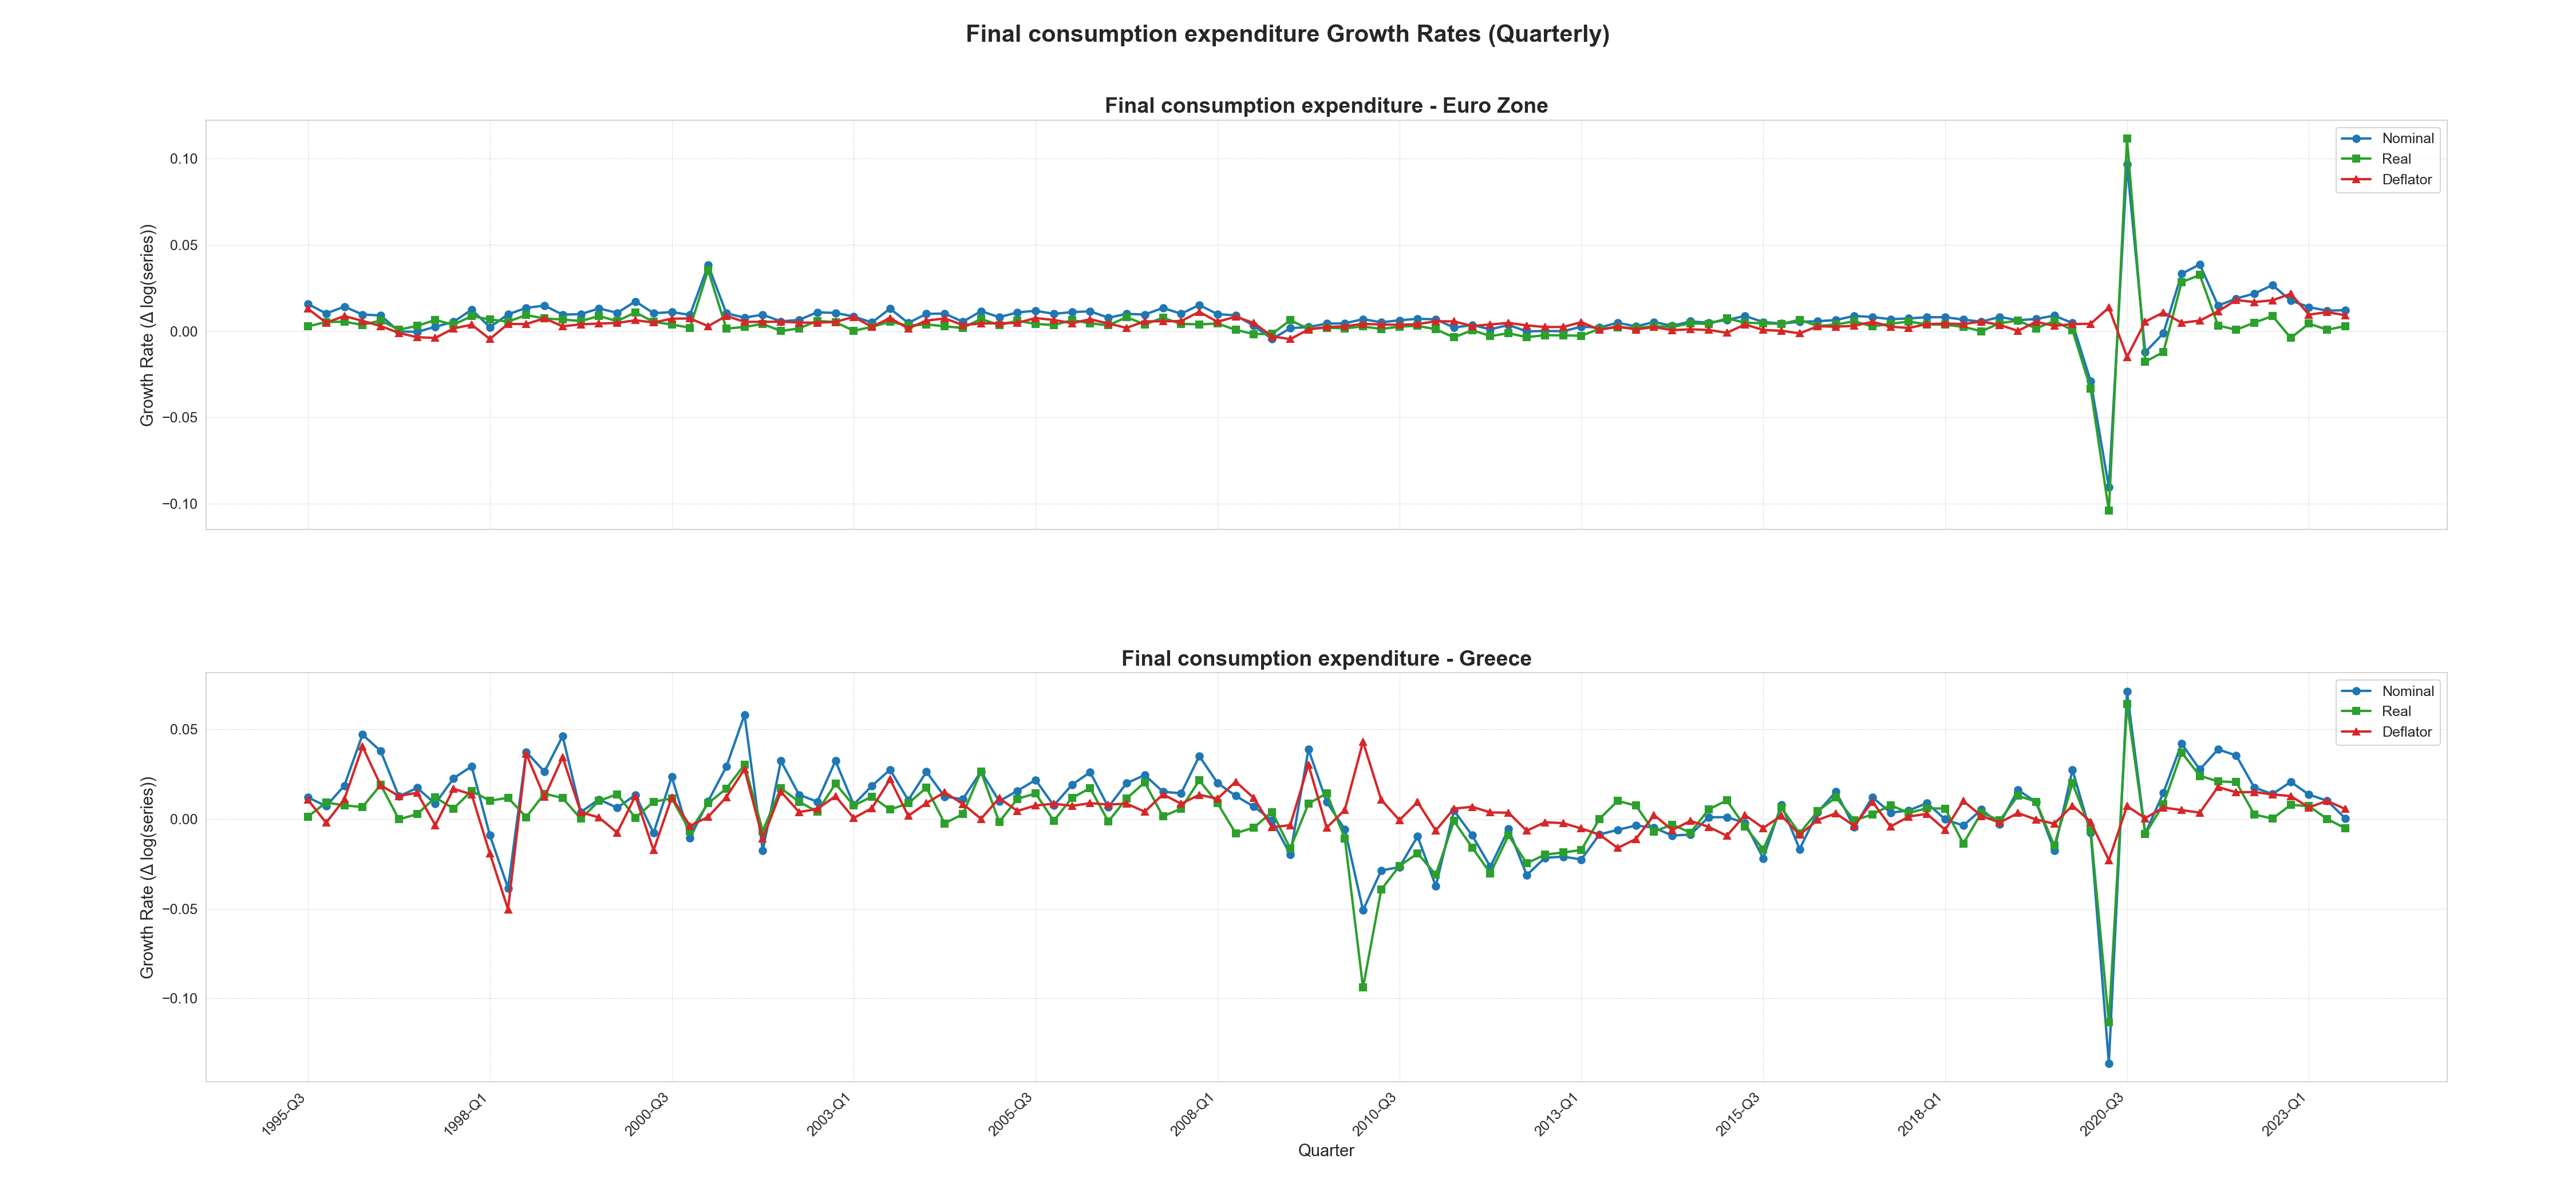
\includegraphics[width=0.8\textwidth]{Final_consumption_expenditure_combined_growth.png}
  \vspace{0.5em}

\captionof{figure}{}\end{tcolorbox}
\FloatBarrier

\section{Ακαθάριστο Εγχώριο Προϊόν σε Τρέχουσες Τιμές Αγοράς: Συνδυασμένη Ανάπτυξη}
\begin{tcolorbox}[colback=white,colframe=black,title={Gross domestic product at market prices: combined growth}]
  \centering
  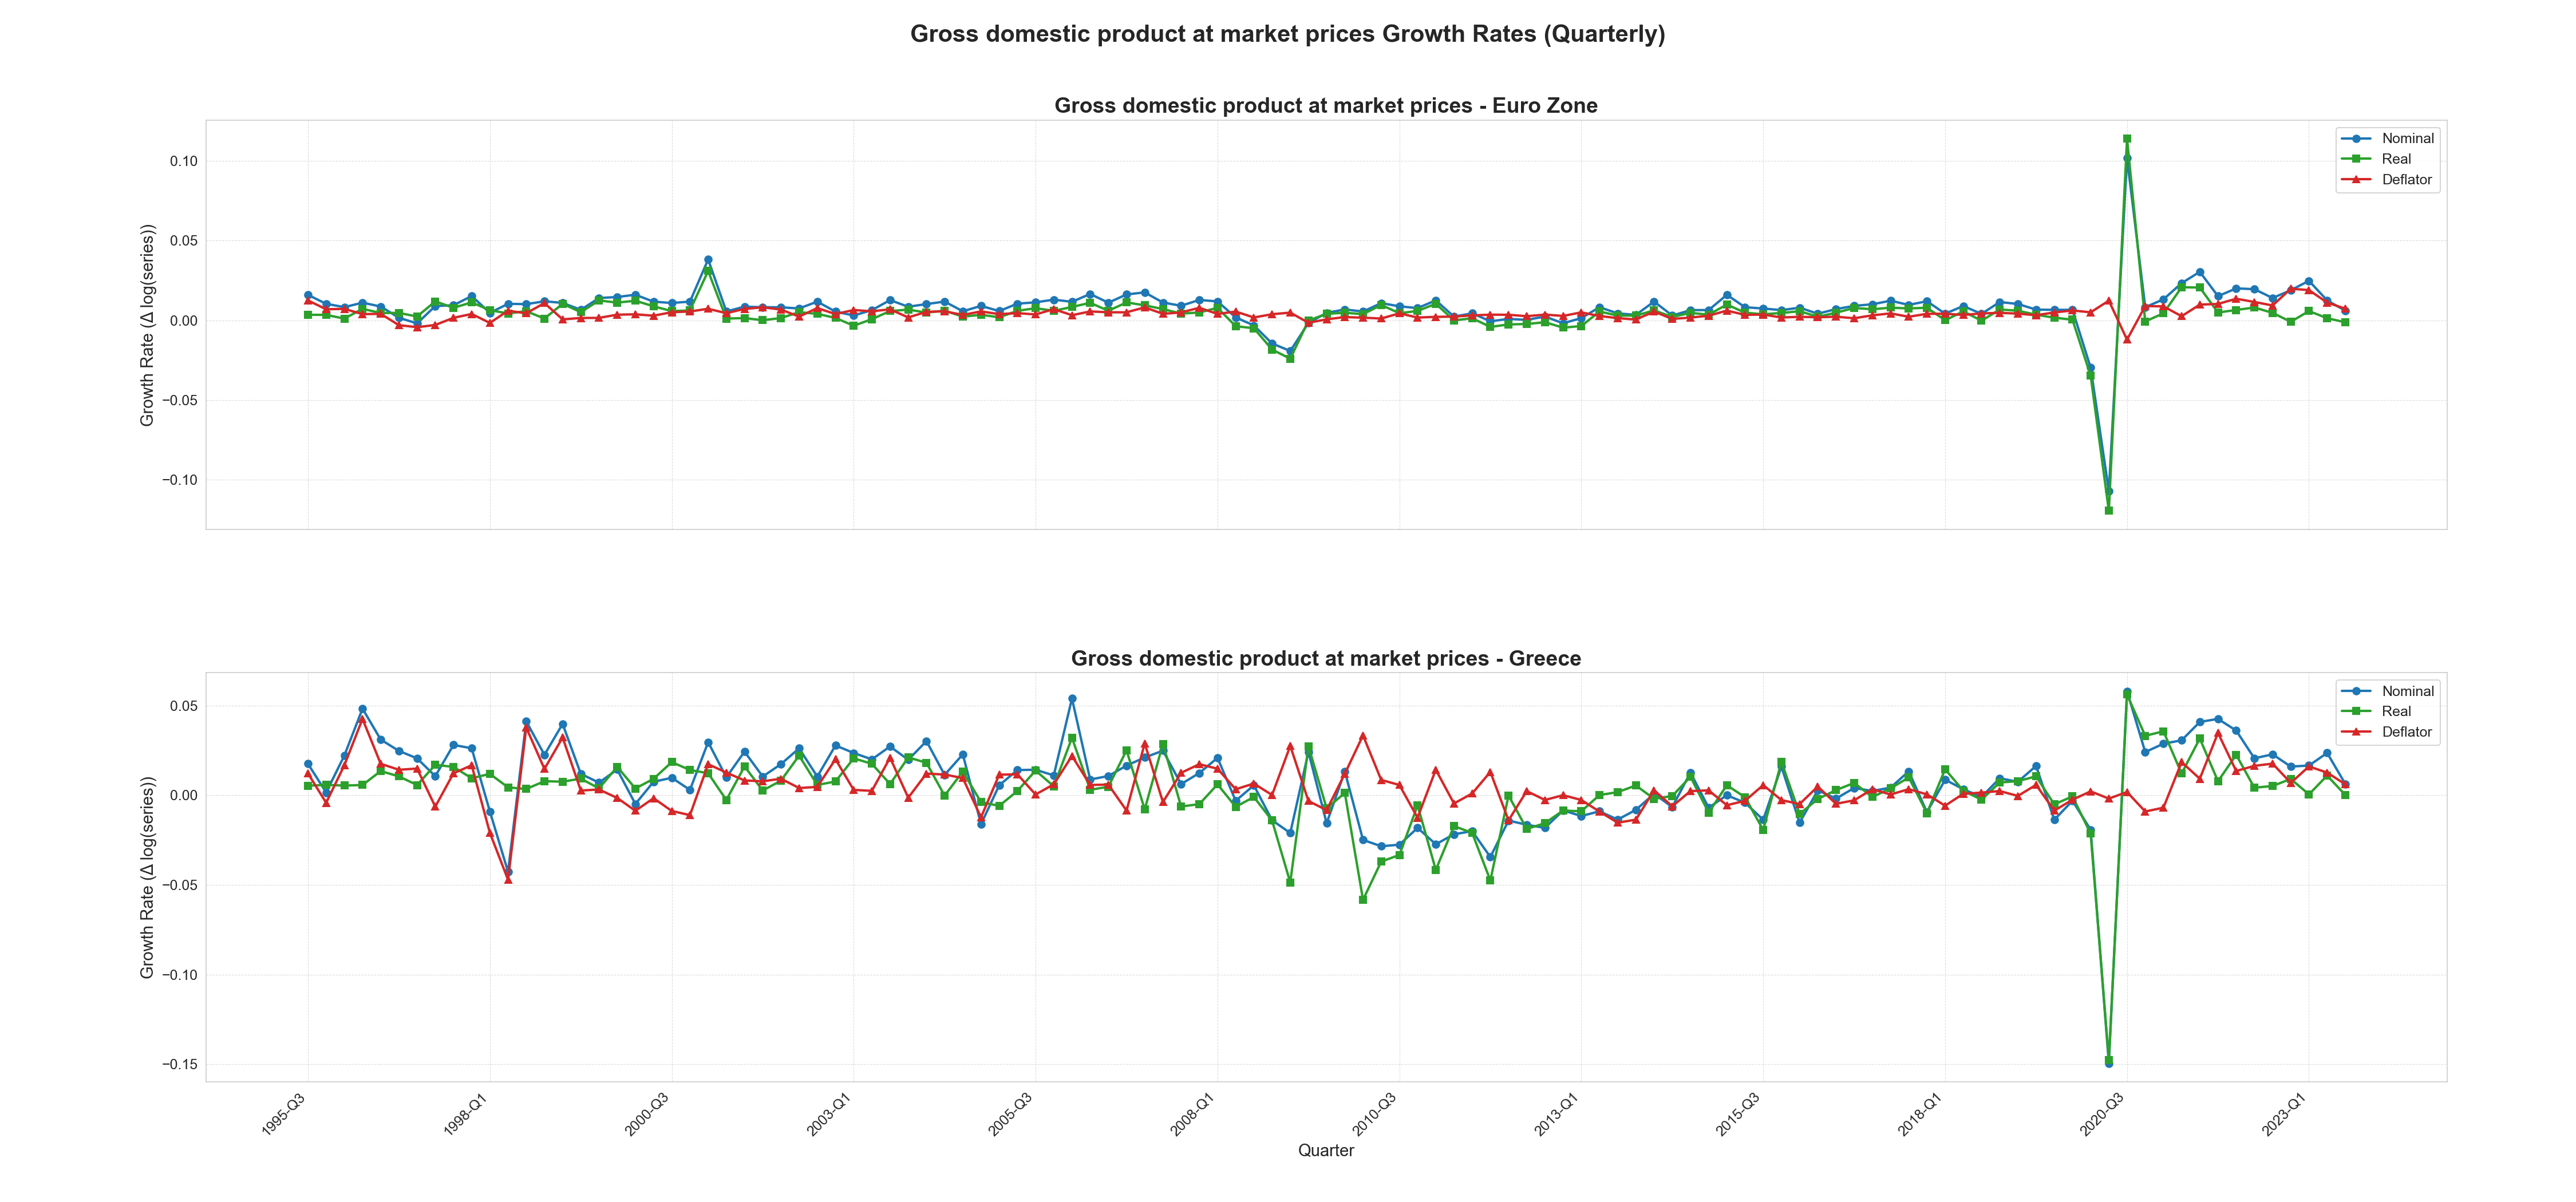
\includegraphics[width=0.8\textwidth]{Gross_domestic_product_at_market_prices_combined_growth.png}
  \vspace{0.5em}

\captionof{figure}{}\end{tcolorbox}
\FloatBarrier

\section{Ακαθάριστος Σχηματισμός Παγίου Κεφαλαίου: Συνδυασμένη Ανάπτυξη}
\begin{tcolorbox}[colback=white,colframe=black,title={Gross fixed capital formation: combined growth}]
  \centering
  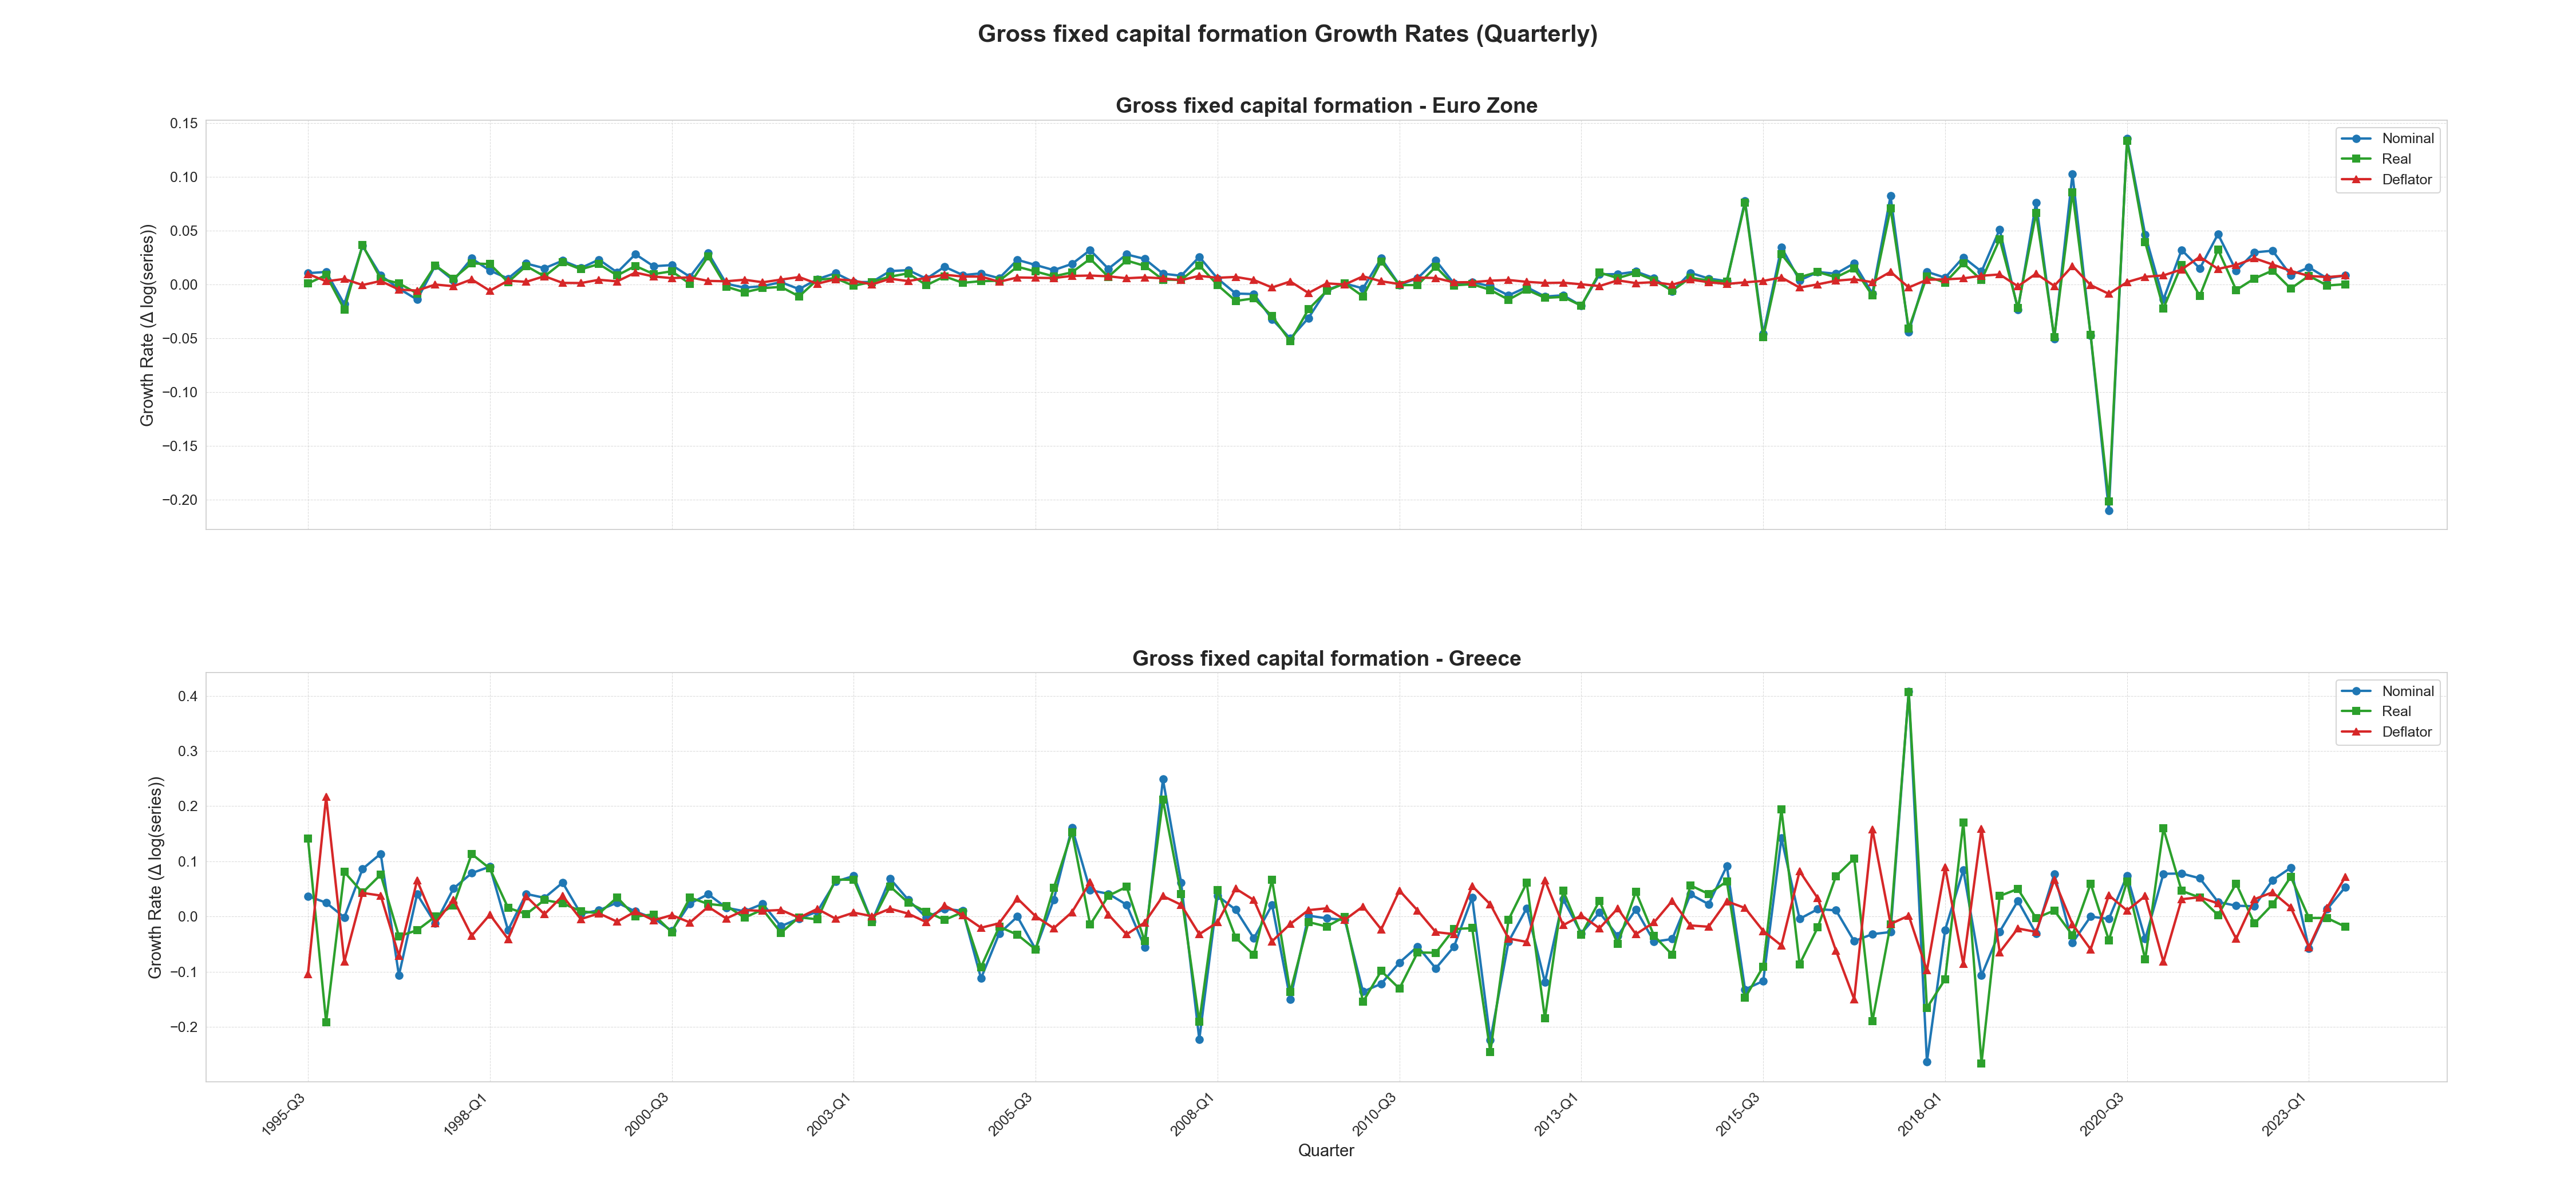
\includegraphics[width=0.8\textwidth]{Gross_fixed_capital_formation_combined_growth.png}
  \vspace{0.5em}

\captionof{figure}{}\end{tcolorbox}
\FloatBarrier
\chapter{Εισαγωγή στην Άσκηση 6}
Η Άσκηση 6 του \emph{MT2 Data Assignment} απαιτεί την αποσύνθεση βασικών μακροοικονομικών σειρών σε συνιστώσες τάσης και κύκλου, χρησιμοποιώντας το \emph{HP-Filter} (Hodrick-Prescott). Συγκεκριμένα, οι ενέργειες που υλοποιούνται είναι:
\begin{itemize}
  \item \textbf{Φόρτωση πραγματικών δεδομένων} για ΑΕΠ, ιδιωτική κατανάλωση (νοικοκυριά) και επενδύσεις (ακαθάριστο σχηματισμό παγίου κεφαλαίου).
  \item \textbf{Εφαρμογή του HP-Filter} με παράμετρο ομαλοποίησης \(\lambda = 1600\) (τυπική επιλογή για τριμηνιαία δεδομένα).
  \item \textbf{Δημιουργία γραφημάτων} που εμφανίζουν:
    \begin{enumerate}
      \item Την πραγματική σειρά σε σύγκριση με την τάση της.
      \item Την κυκλική συνιστώσα (cycle).
      \item Ένα συνδυαστικό γράφημα με τις κυκλικές συνιστώσες διαφορετικών μεταβλητών.
    \end{enumerate}
  \item \textbf{Υπολογισμό μεταβλητότητας} (τυπική απόκλιση) του κύκλου κάθε μεταβλητής και της σχετικής μεταβλητότητας ως προς το ΑΕΠ.
  \item \textbf{Παρουσίαση αποτελεσμάτων} μέσω συνοπτικών πινάκων (CSV) και γραφημάτων.
\end{itemize}

\section{Δομή του Κώδικα}
Το script (\texttt{exercise\_6.py}) χωρίζεται στα εξής μέρη:
\begin{enumerate}
    \item \textbf{Φόρτωση Δεδομένων}: Διαβάζονται οι σειρές από το Excel (π.χ. \texttt{Quarterly\_Data.xlsx}) και κρατούνται οι τρεις μεταβλητές (ΑΕΠ, Ιδιωτική Κατανάλωση, Επενδύσεις).
    \item \textbf{HP-Filter}: Εφαρμόζεται το \texttt{hpfilter} της βιβλιοθήκης \texttt{statsmodels} για την αποσύνθεση κάθε σειράς σε τάση και κύκλο.
    \item \textbf{Δημιουργία Γραφημάτων}:
    \begin{itemize}
        \item Πραγματική σειρά vs. τάση (ανά χώρα).
        \item Κυκλική συνιστώσα (ανά χώρα).
        \item Συνδυαστικά γραφήματα με όλες τις κυκλικές συνιστώσες.
    \end{itemize}
    \item \textbf{Μεταβλητότητα}: Υπολογίζεται η τυπική απόκλιση των κυκλικών συνιστωσών και η σχετική μεταβλητότητα ως προς το ΑΕΠ.
    \item \textbf{Αποθήκευση Αποτελεσμάτων}: Δημιουργία CSV και αποθήκευση γραφημάτων.
\end{enumerate}

%==============================
% Chapter 2: Code Overview
%==============================
\section{ Κώδικας (exercise\_6.py): Ανάλυση με HP-Filter}
\subsection{Παράδειγμα Συναρτήσεων – Φόρτωση \& Αποσύνθεση}
\begin{tcolorbox}[colback=white,colframe=black,title=Υπόδειγμα Φόρτωσης και Εφαρμογής HP-Filter (Pseudo-code)]
\begin{lstlisting}[language=Python]
import pandas as pd
import numpy as np
import matplotlib.pyplot as plt
from statsmodels.tsa.filters.hp_filter import hpfilter

...

def apply_hpfilter(series, lamb=1600):
    """
    Εφαρμόζει το HP-Filter σε μια Pandas Series.
    Επιστρέφει τις συνιστώσες (cycle, trend).
    """
    cycle, trend = hpfilter(series, lamb=lamb)
    return cycle, trend
\end{lstlisting}
\end{tcolorbox}

\section{Σχεδίαση Γραφημάτων: Actual vs. Trend και Cycle}
\begin{tcolorbox}[colback=white,colframe=black,title=Παράδειγμα Σχεδιασμού (Actual vs. Trend και Cycle)]
\begin{lstlisting}[language=Python]
def plot_actual_vs_trend_and_cycle(df, var_name):
    """
    Δημιουργεί δύο σύνολα διαγραμμάτων:
    1. Πραγματική σειρά και τάση για Euro και Ελλάδα.
    2. Κυκλική συνιστώσα για Euro και Ελλάδα.
    """
    cycle_euro, trend_euro = apply_hpfilter(df["Euro"])
    cycle_gr, trend_gr = apply_hpfilter(df["Ελλάδα"])

    # Πραγματική σειρά vs. Τάση
    fig, axs = plt.subplots(2, 1, figsize=(12, 8), sharex=True)
    axs[0].plot(df.index, df["Euro"], label="Euro (Actual)", marker='o')
    axs[0].plot(df.index, trend_euro, label="Euro (Trend)", linestyle='--')
    axs[0].set_title(var_name + " - Euro")
    axs[1].plot(df.index, df["Ελλάδα"], label="Ελλάδα (Actual)", marker='o')
    axs[1].plot(df.index, trend_gr, label="Ελλάδα (Trend)", linestyle='--')
    axs[1].set_title(var_name + " - Ελλάδα")
    plt.legend()
    plt.tight_layout()
    plt.savefig(var_name + "_Πραγματική_και_Τάση.png")
    plt.close()

    # Κυκλική Συνιστώσα
    fig2, axs2 = plt.subplots(2, 1, figsize=(12, 8), sharex=True)
    axs2[0].plot(df.index, cycle_euro, label="Euro (Cycle)", marker='o')
    axs2[0].set_title(var_name + " Κυκλική - Euro")
    axs2[1].plot(df.index, cycle_gr, label="Ελλάδα (Cycle)", marker='o')
    axs2[1].set_title(var_name + " Κυκλική - Ελλάδα")
    plt.legend()
    plt.tight_layout()
    plt.savefig(var_name + "_Κυκλική.png")
    plt.close()
\end{lstlisting}
\end{tcolorbox}

\section{Συνδυαστικά Γραφήματα για Όλες τις Κυκλικές Συνιστώσες}
\begin{tcolorbox}[colback=white,colframe=black,title=Ομαδική Απεικόνιση των Κυκλικών Στοιχείων]
\begin{lstlisting}[language=Python]
def plot_all_cycles(cycles_dict, region, filename):
    """
    cycles_dict: {"GDP": df_cycle, "Consumption": df_cycle, "Investment": df_cycle}
    Κάθε df_cycle έχει στήλες "Euro" και "Ελλάδα".
    """
    plt.figure(figsize=(14,6))
    for var_name, df_cycle in cycles_dict.items():
        plt.plot(df_cycle.index, df_cycle[region], marker='o', label=var_name)
    plt.title(f"Κυκλικές Συνιστώσες - {region}")
    plt.legend()
    plt.savefig(filename)
    plt.close()
\end{lstlisting}
\end{tcolorbox}

\section{Υπολογισμός Μεταβλητότητας και Σχετικής Μεταβλητότητας}
\begin{tcolorbox}[colback=white,colframe=black,title=Εξαγωγή Τυπικής Απόκλισης και Σχετικής Μεταβλητότητας]
\begin{lstlisting}[language=Python]
def compute_relative_volatility(cycles_dict):
    """
    cycles_dict: {"GDP": df_cycle_gdp, "Consumption": df_cycle_con, ...}
    Επιστρέφει δύο DataFrames:
      - rel_vol_euro: για την Ευρωζώνη
      - rel_vol_gr: για την Ελλάδα
    Κάθε DataFrame περιέχει τις στήλες:
      [Μεταβλητή, Μεταβλητότητα, Σχετική Μεταβλητότητα (ως προς ΑΕΠ)]
    """
    stdevs_euro = {}
    stdevs_gr = {}
    for var, df_cycle in cycles_dict.items():
        stdevs_euro[var] = df_cycle["Euro"].std()
        stdevs_gr[var]   = df_cycle["Ελλάδα"].std()

    gdp_euro_std = stdevs_euro["GDP"]
    gdp_gr_std   = stdevs_gr["GDP"]

    data_euro = []
    data_gr = []
    for var in cycles_dict.keys():
        vol_euro = stdevs_euro[var]
        vol_gr = stdevs_gr[var]
        rel_euro = vol_euro / gdp_euro_std if gdp_euro_std != 0 else None
        rel_gr = vol_gr / gdp_gr_std if gdp_gr_std != 0 else None
        data_euro.append([var, vol_euro, rel_euro])
        data_gr.append([var, vol_gr, rel_gr])

    df_euro = pd.DataFrame(data_euro, columns=["Μεταβλητή", "Μεταβλητότητα", "Σχετική Μεταβλητότητα"])
    df_gr = pd.DataFrame(data_gr, columns=["Μεταβλητή", "Μεταβλητότητα", "Σχετική Μεταβλητότητα"])
    return df_euro, df_gr
\end{lstlisting}
\end{tcolorbox}

%==============================
% Chapter 3: Appendix: Tables & Plots
%==============================
\section{Παράρτημα: Πίνακες \& Γραφήματα (Άσκηση 6)}

\subsection{Πίνακες Μεταβλητότητας από CSV}
Σε αυτήν την ενότητα παρουσιάζουμε τους πίνακες με τη σχετική μεταβλητότητα, που έχουν παραχθεί και αποθηκευτεί ως CSV.

\subsection{Σχετική Μεταβλητότητα: Ευρωζώνη}
\begin{table}[h!]
\centering
\caption{Relative Volatility - Euro}
\csvautobooktabular[
    separator=comma,         % Αν τα δεδομένα είναι διαχωρισμένα με κόμμα
    respect all
]{/Users/thodoreskourtales/TK.MT.1/exercise.6/relative_volatility_Euro.csv}
\end{table}
\FloatBarrier

\subsection{Σχετική Μεταβλητότητα: Ελλάδα}
\begin{table}[h!]
\centering
\caption{Relative Volatility - Ελλάδα}
\csvautobooktabular[
    separator=comma,
    respect all
]{/Users/thodoreskourtales/TK.MT.1/exercise.6/relative_volatility_Ελλάδα.csv}
\end{table}
\FloatBarrier

\section{Γραφήματα από την Αποσύνθεση HP-Filter}
Παρακάτω παρουσιάζονται τα γραφήματα που παράγει το script, τα οποία απεικονίζουν τις κυκλικές συνιστώσες και τις αποσυνθέσεις (πραγματική σειρά, τάση, κύκλος).
\graphicspath{{/Users/thodoreskourtales/TK.MT.1/exercise.6/}}
\subsection{Όλες οι Κυκλικές Συνιστώσες}
\begin{tcolorbox}[colback=white,colframe=black,title={Όλες οι Κυκλικές Συνιστώσες - Ευρωζώνη}]
  \centering
  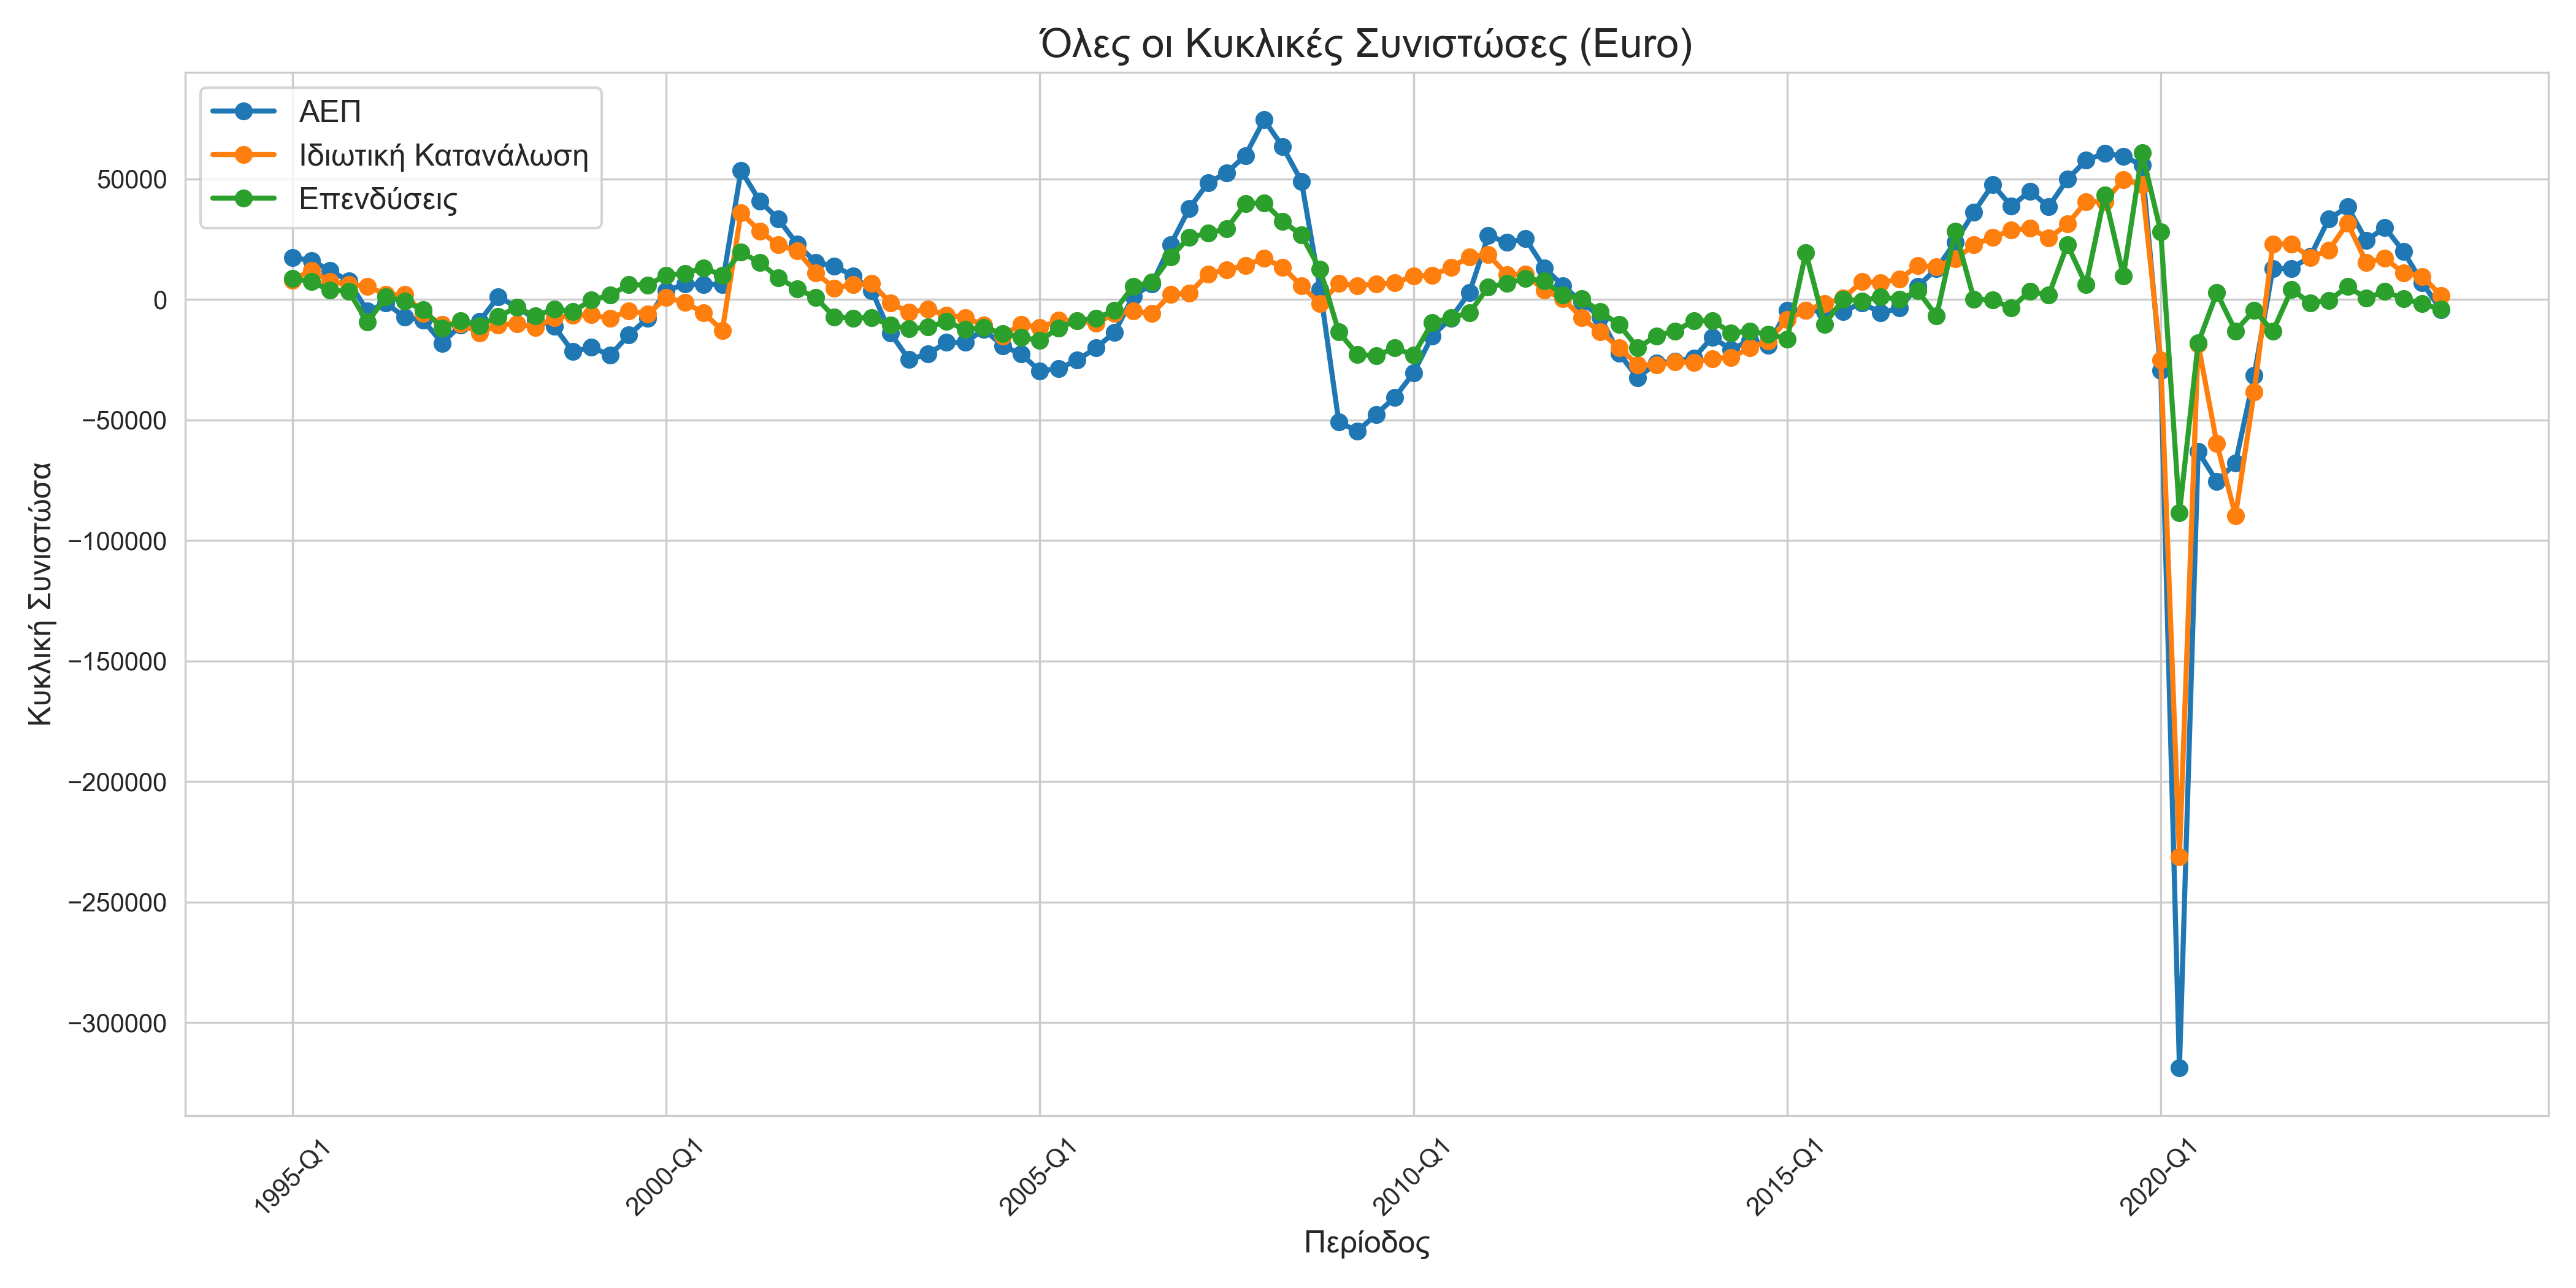
\includegraphics[width=0.8\textwidth]{all_cyclical_components_Euro.png}
  \vspace{0.5em}

\captionof{figure}{}\end{tcolorbox}
\FloatBarrier

\begin{tcolorbox}[colback=white,colframe=black,title={Όλες οι Κυκλικές Συνιστώσες - Ελλάδα}]
  \centering
  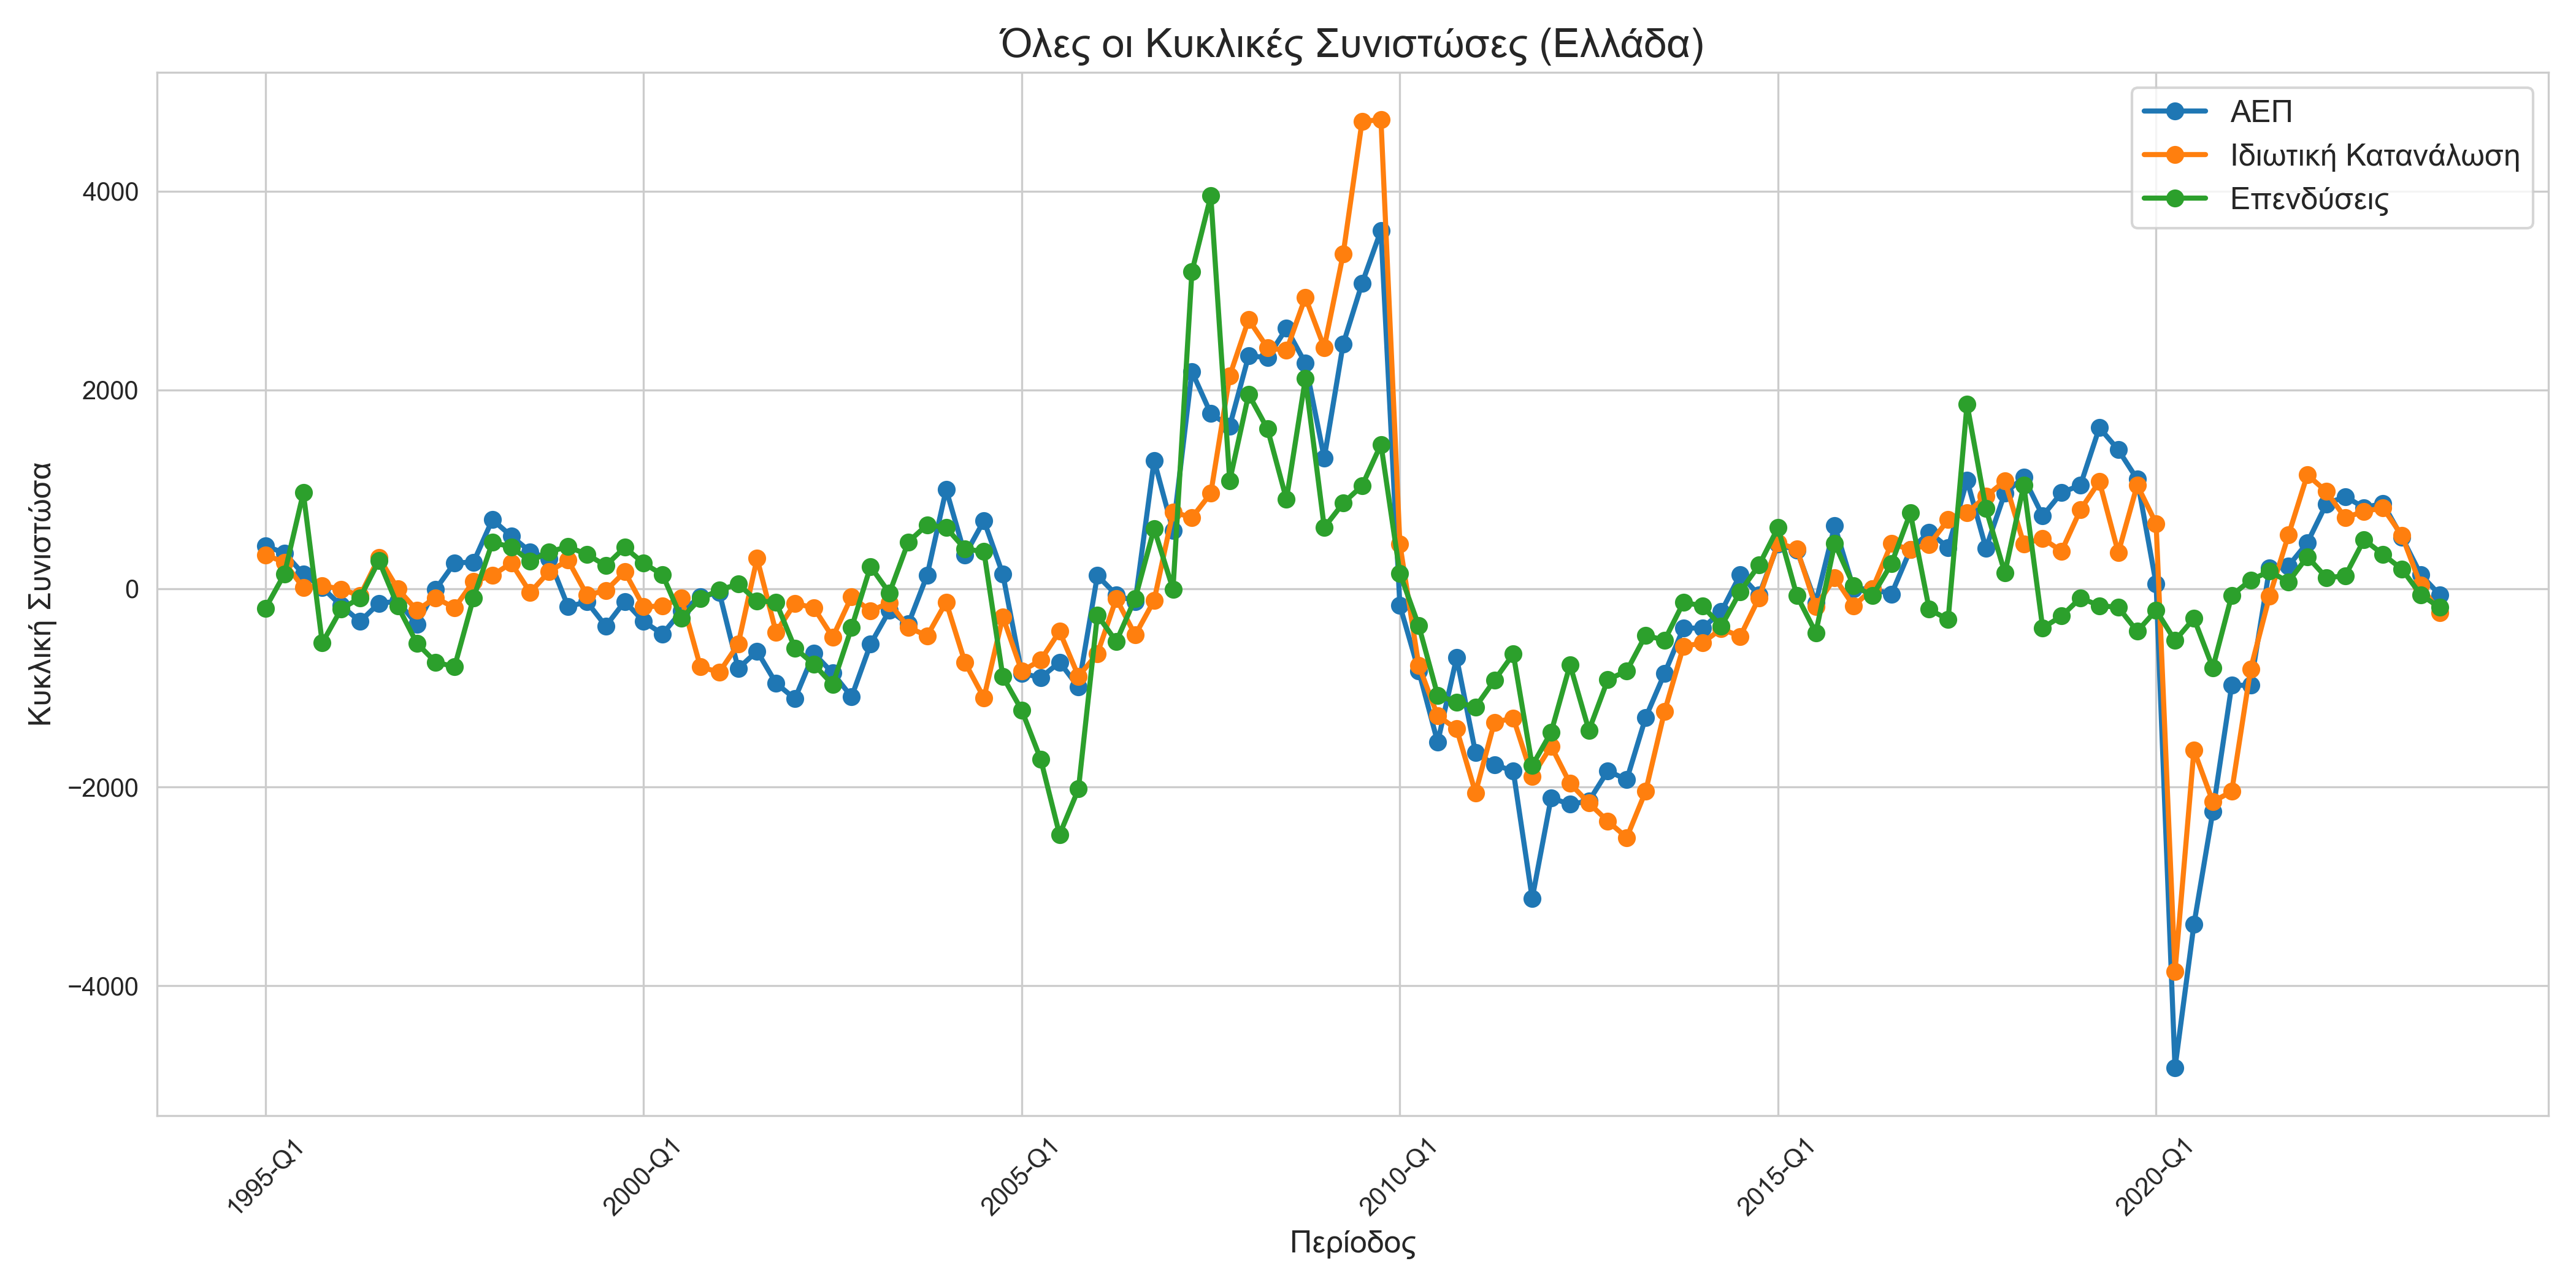
\includegraphics[width=0.8\textwidth]{all_cyclical_components_Ελλάδα.png}
  \vspace{0.5em}

\captionof{figure}{}\end{tcolorbox}
\FloatBarrier

\subsection{Ακαθάριστο Εγχώριο Προϊόν (ΑΕΠ)}
\begin{tcolorbox}[colback=white,colframe=black,title={ΑΕΠ - Κυκλική Συνιστώσα}]
  \centering
  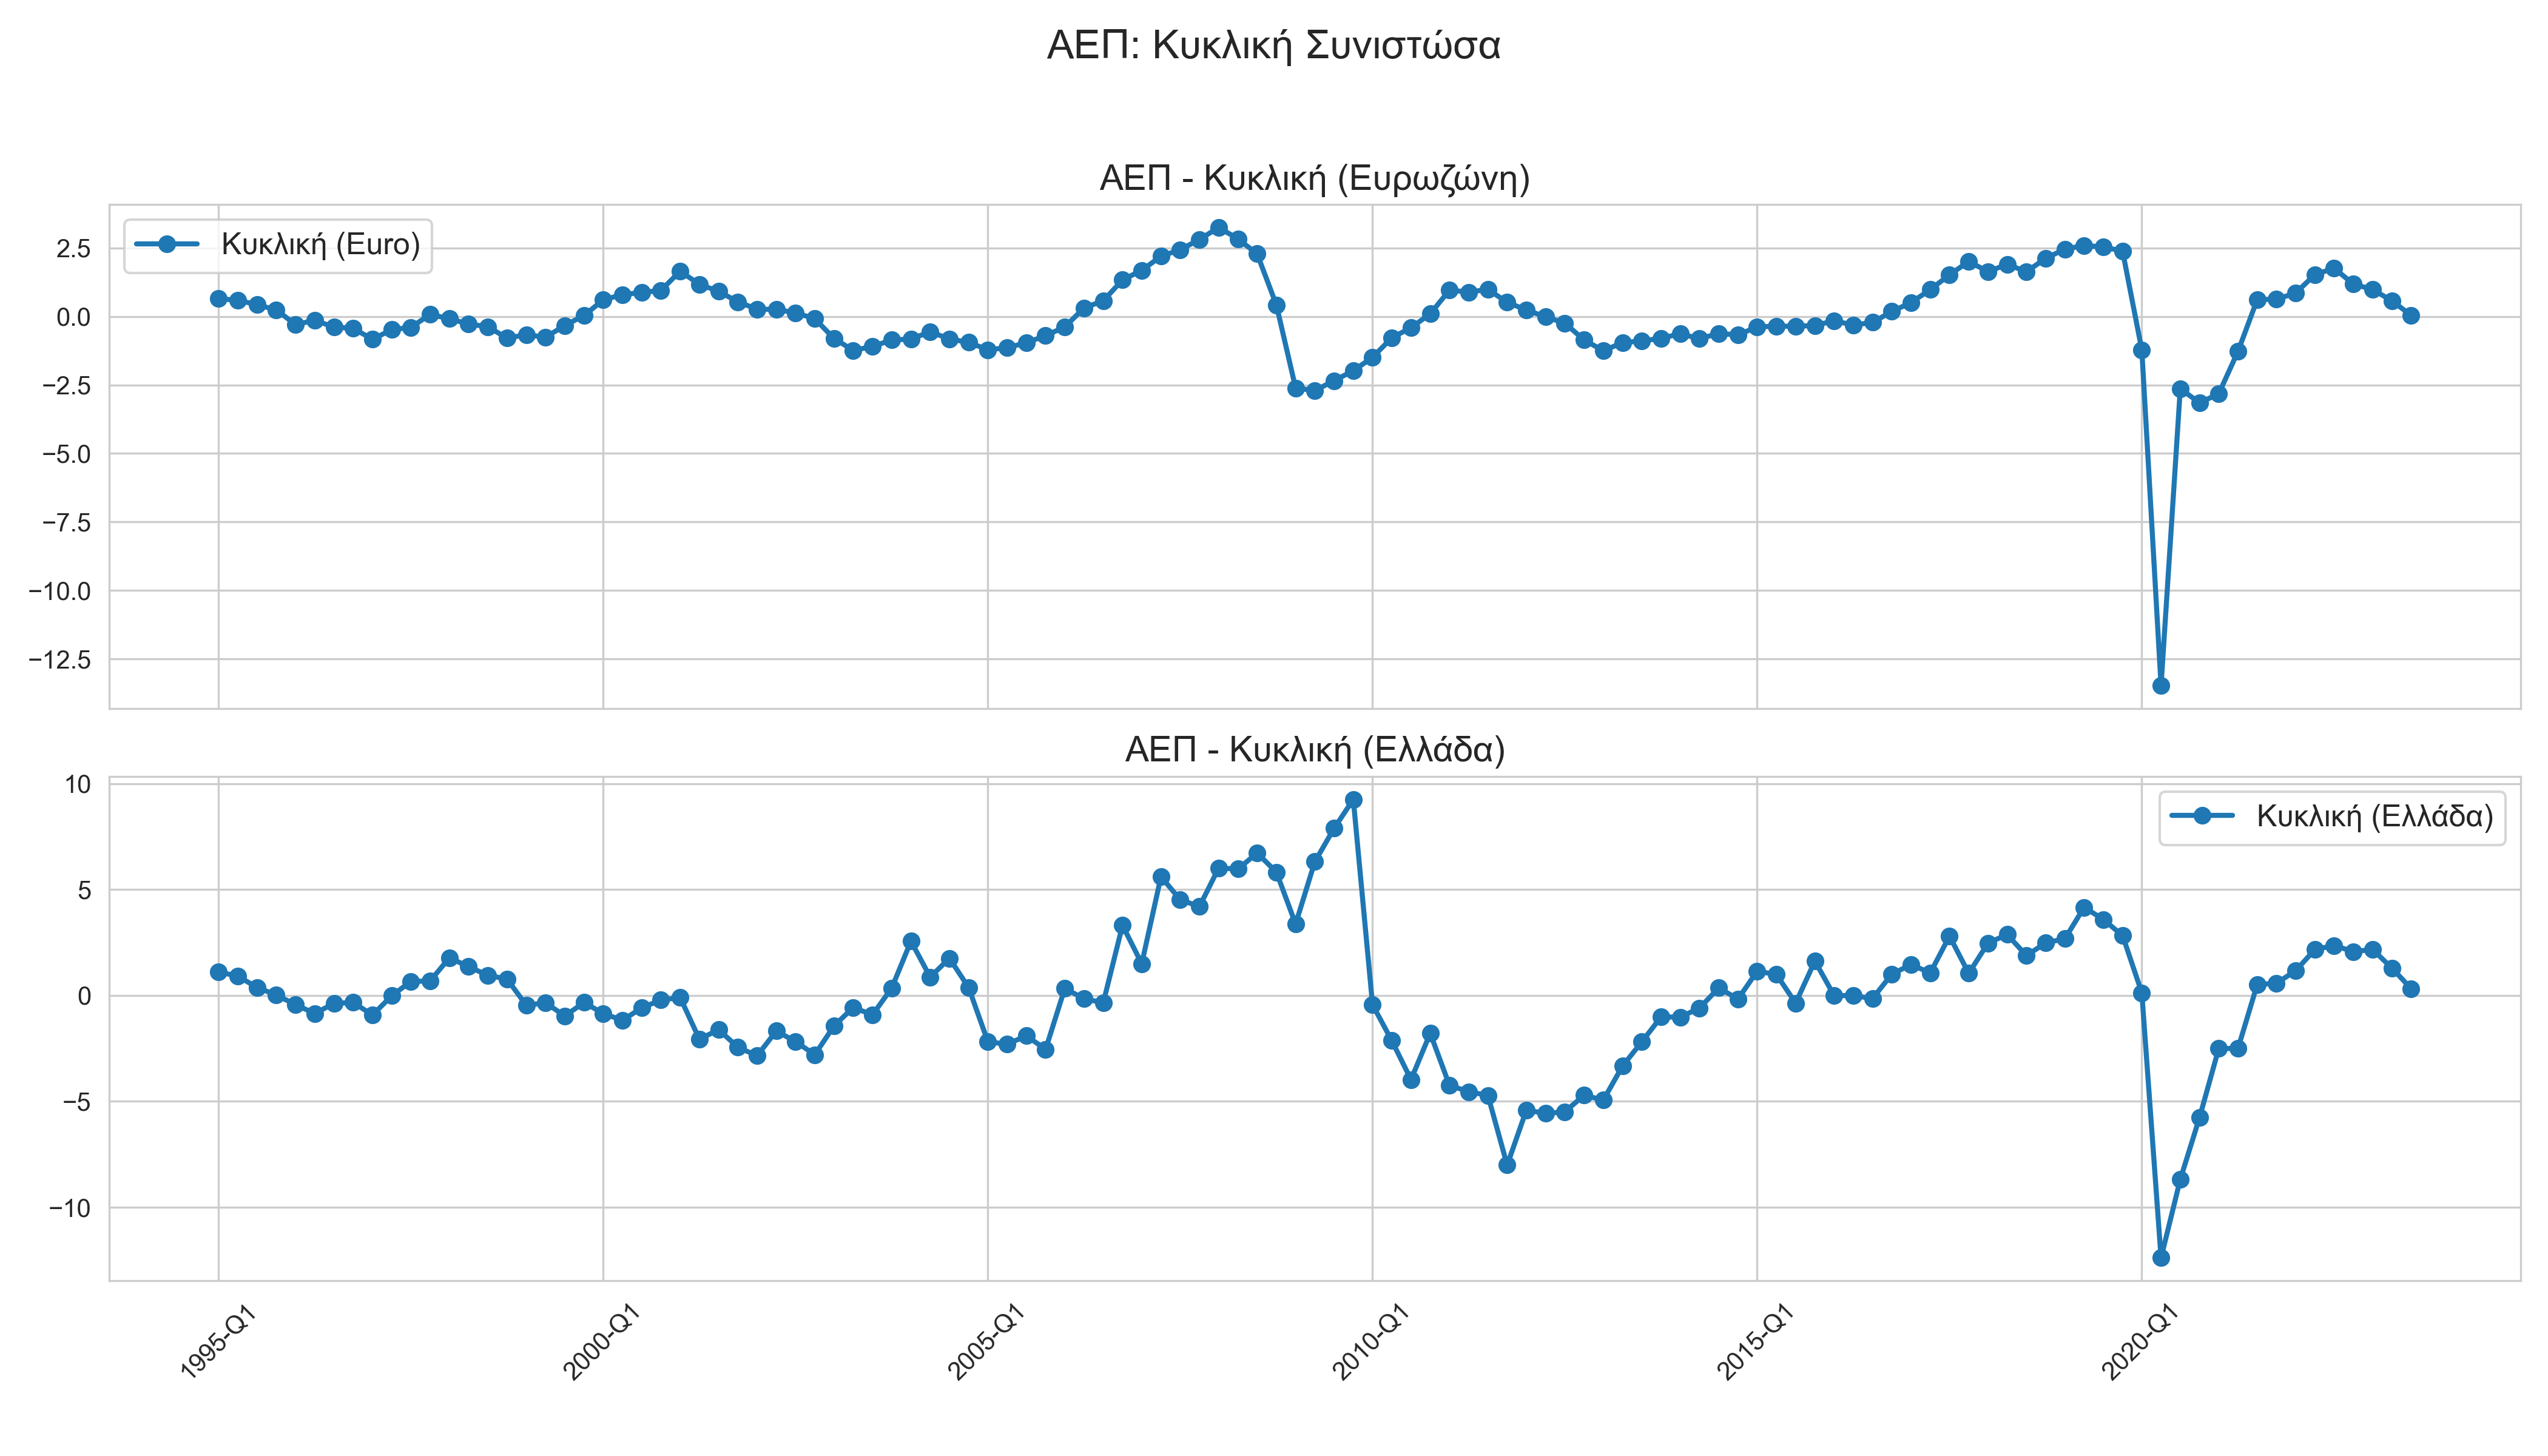
\includegraphics[width=0.8\textwidth]{ΑΕΠ_Κυκλική.png}
  \vspace{0.5em}

\captionof{figure}{}\end{tcolorbox}
\FloatBarrier

\begin{tcolorbox}[colback=white,colframe=black,title={ΑΕΠ - Πραγματική και Τάση}]
  \centering
  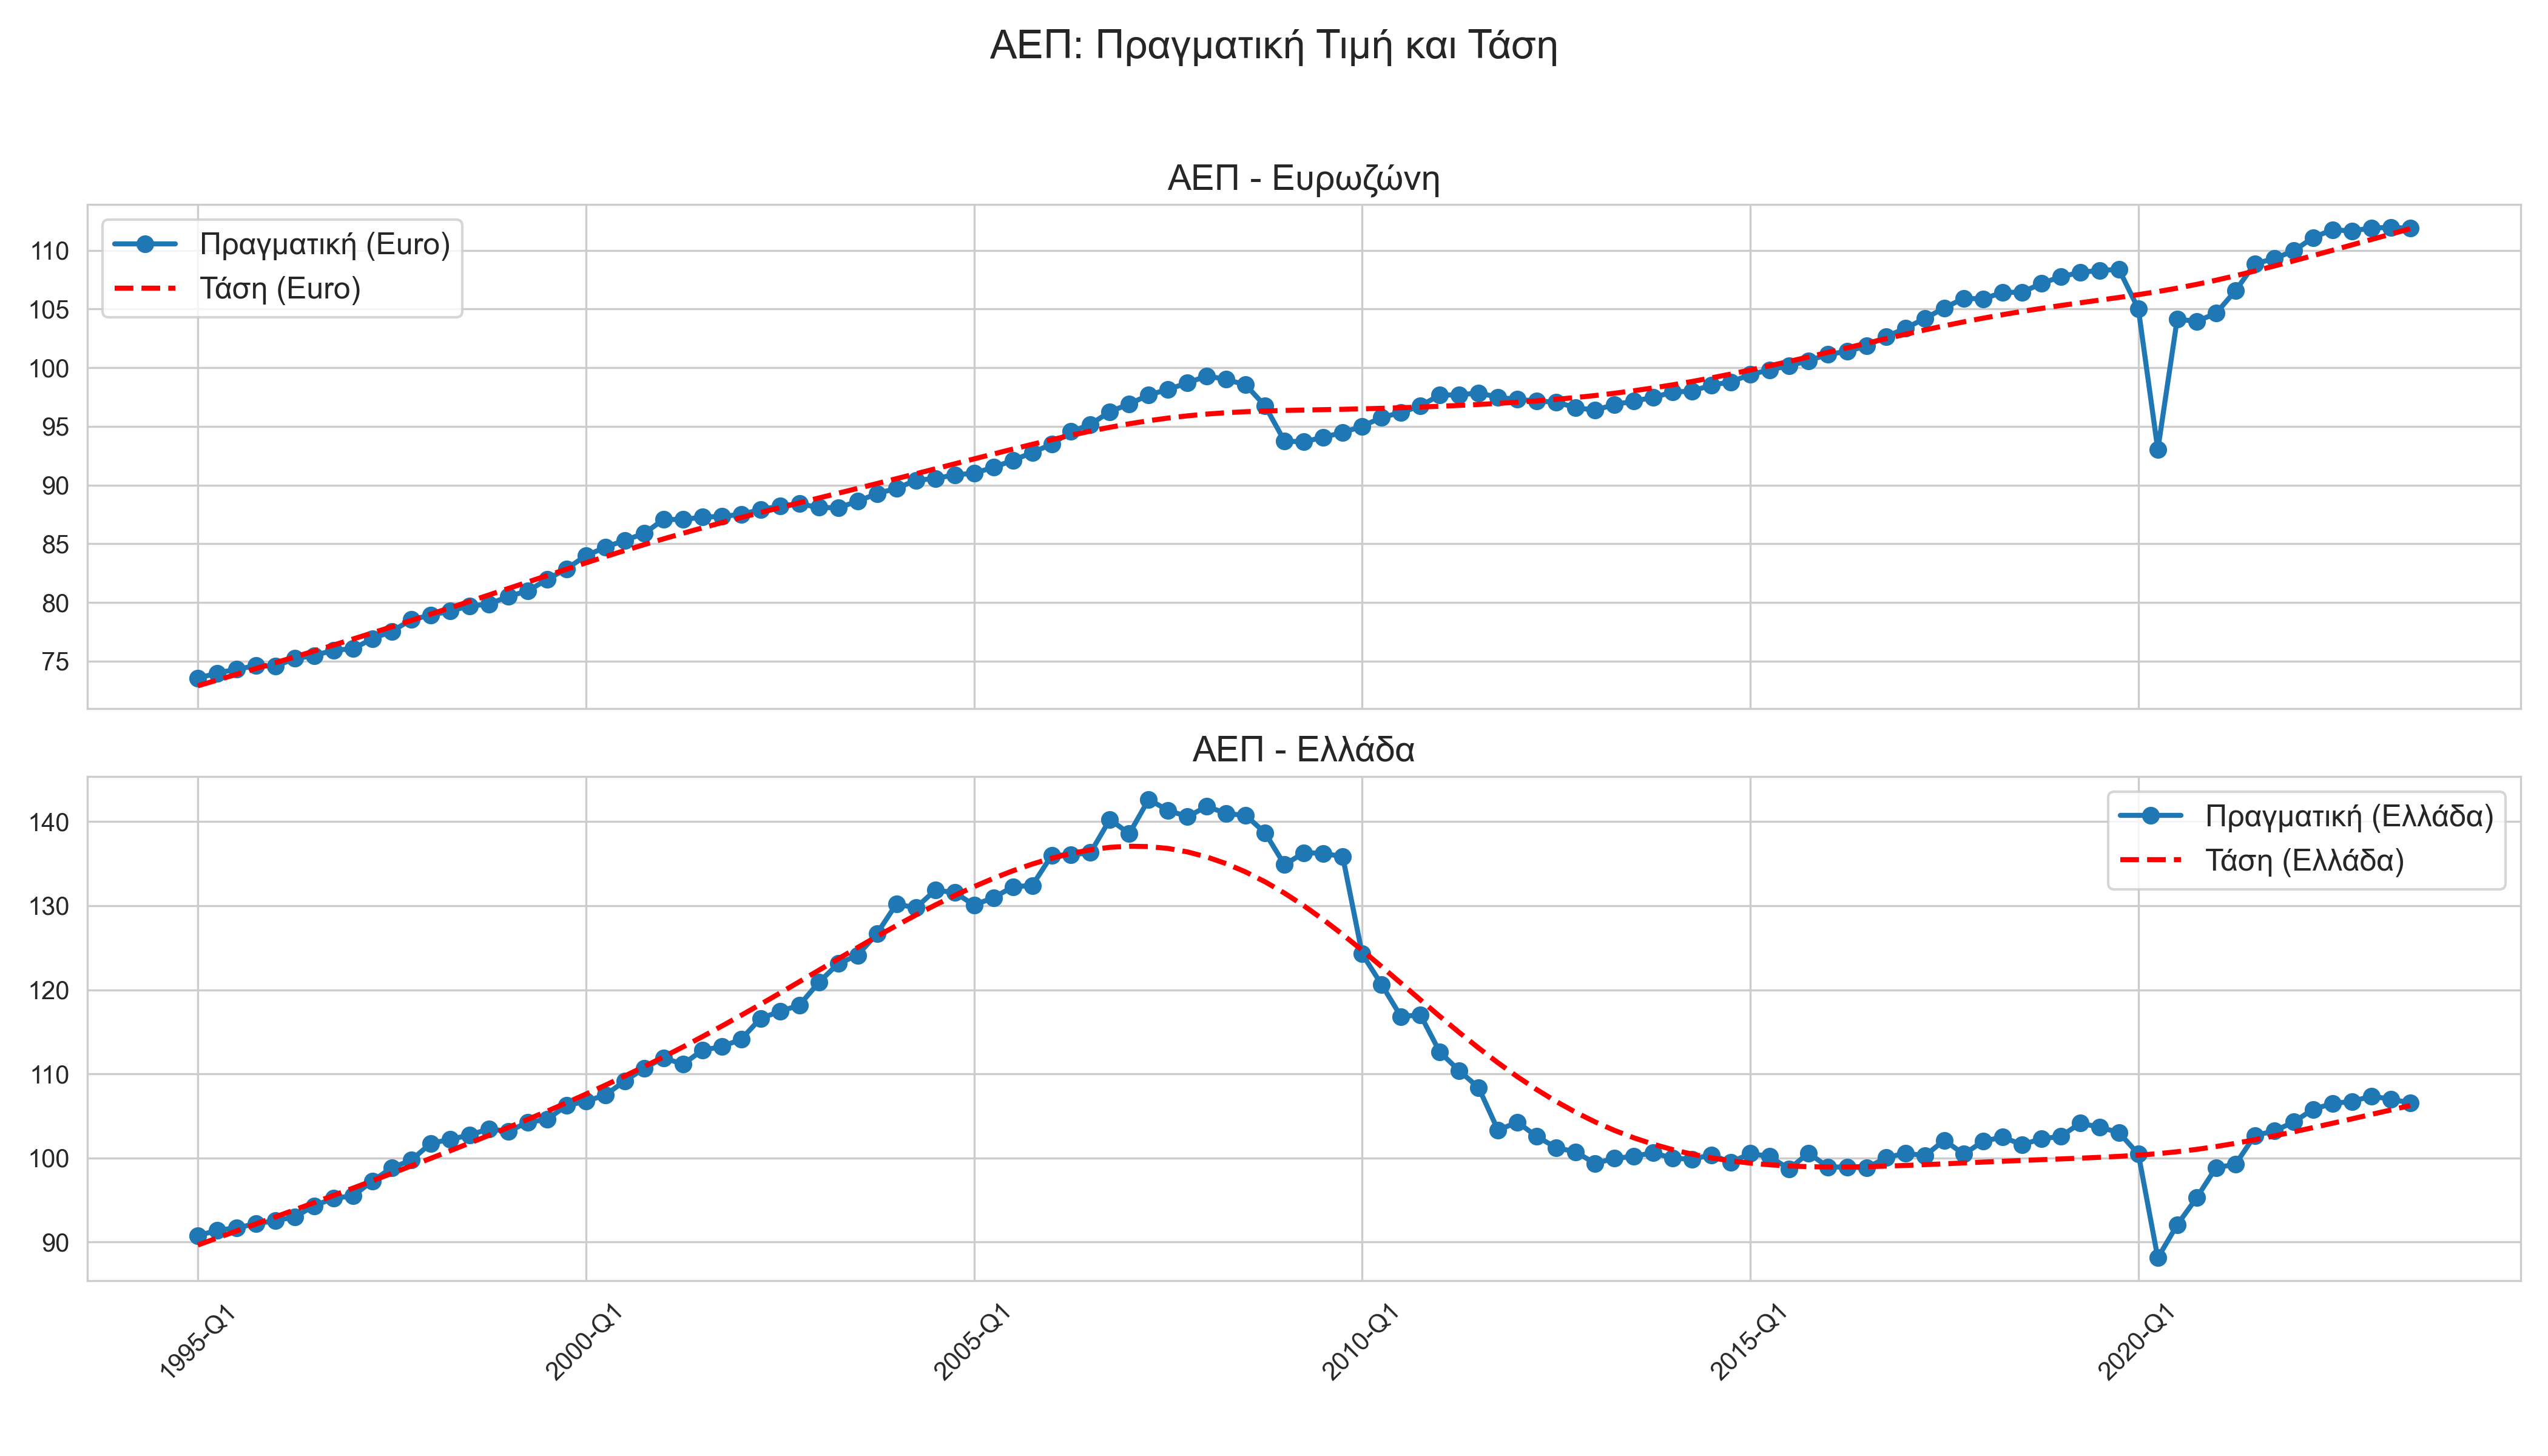
\includegraphics[width=0.8\textwidth]{ΑΕΠ_Πραγματική_και_Τάση.png}
  \vspace{0.5em}

\captionof{figure}{}\end{tcolorbox}
\FloatBarrier

\subsection{Επενδύσεις}
\begin{tcolorbox}[colback=white,colframe=black,title={Επενδύσεις - Κυκλική Συνιστώσα}]
  \centering
  \includegraphics[width=0.8\textwidth]{Επενδύσεις_Κυκλική.png}
  \vspace{0.5em}

\captionof{figure}{}\end{tcolorbox}
\FloatBarrier

\begin{tcolorbox}[colback=white,colframe=black,title={Επενδύσεις - Πραγματική και Τάση}]
  \centering
  \includegraphics[width=0.8\textwidth]{Επενδύσεις_Πραγματική_και_Τάση.png}
  \vspace{0.5em}

\captionof{figure}{}\end{tcolorbox}
\FloatBarrier

\subsection{Ιδιωτική Κατανάλωση}
\begin{tcolorbox}[colback=white,colframe=black,title={Ιδιωτική Κατανάλωση - Κυκλική Συνιστώσα}]
  \centering
  \includegraphics[width=0.8\textwidth]{Ιδιωτική_Κατανάλωση_Κυκλική.png}
  \vspace{0.5em}

\captionof{figure}{}\end{tcolorbox}
\FloatBarrier

\begin{tcolorbox}[colback=white,colframe=black,title={Ιδιωτική Κατανάλωση - Πραγματική και Τάση}]
  \centering
  \includegraphics[width=0.8\textwidth]{Ιδιωτική_Κατανάλωση_Πραγματική_και_Τάση.png}
  \vspace{0.5em}

\captionof{figure}{}\end{tcolorbox}
\FloatBarrier

\end{document}